%%%%%%%%%%%%%%%%%%%%%%%%%%%%%%%%%%%%%%%%%%%%%%%%%%%%%%%%%%%%%%%%%%%%%%%%%%%%%%%%%%%%%%%%%%%%%%%%
%                                                                                              %
%                             Definicao para a classe Artigo                                   %
%                                                                                              %
%%%%%%%%%%%%%%%%%%%%%%%%%%%%%%%%%%%%%%%%%%%%%%%%%%%%%%%%%%%%%%%%%%%%%%%%%%%%%%%%%%%%%%%%%%%%%%%%

\documentclass[portugues, brazil, a4paper,12pt]{article}
\bibliographystyle{plain}

%%%%%%%%%%%%%%%%%%%%%%%%%%%%%%%%%%%%%%%%%%%%%%%%%%%%%%%%%%%%%%%%%%%%%%%%%%%%%%%%%%%%%%%%%%%%%%%%
%                                                                                              %
%                       Pacotes a utilizar na compilacao do documento                          %
%                                                                                              %
%%%%%%%%%%%%%%%%%%%%%%%%%%%%%%%%%%%%%%%%%%%%%%%%%%%%%%%%%%%%%%%%%%%%%%%%%%%%%%%%%%%%%%%%%%%%%%%%

\usepackage[brazil]{babel}
\usepackage{graphicx}
\usepackage{geometry}
\usepackage[utf8]{inputenc}
\usepackage[T1]{fontenc}
\usepackage{epstopdf}
\usepackage{hyperref}
\usepackage{float}
\usepackage{gensymb}
\usepackage{color}
\usepackage{url}

\usepackage{graphicx,url}

\usepackage[brazil]{babel}
\usepackage{verbatim}
\usepackage{todonotes}
\usepackage{longtable}
\usepackage{amssymb}
\usepackage{amsmath}
\usepackage{float}
\usepackage{amsfonts}
\usepackage{algorithm, algpseudocode}
\usepackage{color}
\usepackage{minted}
\usepackage{url}
\usepackage{multicol}
%\usepackage[latin1]{inputenc}
\usepackage[utf8]{inputenc}
\usepackage{longtable}

\hypersetup{
    colorlinks,
    citecolor=black,
    filecolor=black,
    linkcolor=black,
    urlcolor=black
}



\makeatletter
\renewcommand{\paragraph}{\@startsection{paragraph}{4}{0ex}%
   {-3.25ex plus -1ex minus -0.2ex}%
   {1.5ex plus 0.2ex}%
   {\normalfont\normalsize\bfseries}}
\makeatother

\stepcounter{secnumdepth}
\stepcounter{tocdepth}

%%%%%%%%%%%%%%%%%%%%%%%%%%%%%%%%%%%%%%%%%%%%%%%%%%%%%%%%%%%%%%%%%%%%%%%%%%%%%%%%%%%%%%%%%%%%%%%%
%                                                                                              %
%                       Configuracao dos pacotes utilizados no doc.                            %
%                                                                                              %
%%%%%%%%%%%%%%%%%%%%%%%%%%%%%%%%%%%%%%%%%%%%%%%%%%%%%%%%%%%%%%%%%%%%%%%%%%%%%%%%%%%%%%%%%%%%%%%%

\geometry{a4paper,left=3cm,right=3cm,top=2.5cm,bottom=2.93cm}


%%%%%%%%%%%%%%%%%%%%%%%%%%%%%%%%%%%%%%%%%%%%%%%%%%%%%%%%%%%%%%%%%%%%%%%%%%%%%%%%%%%%%%%%%%%%%%%%
%                                                                                              %
%                                   Capa do Documento                                          %
%                                                                                              %
%%%%%%%%%%%%%%%%%%%%%%%%%%%%%%%%%%%%%%%%%%%%%%%%%%%%%%%%%%%%%%%%%%%%%%%%%%%%%%%%%%%%%%%%%%%%%%%%

\begin{document}

\begin{titlepage}

  \vfill

	\begin{figure}[H]
	\centering
		
\includegraphics[scale=0.15]{img/logo-ufop.jpg}
	\end{figure}

  \vfill

  \begin{center}
    \begin{Large}
      \textbf{UNIVERSIDADE FEDERAL DE OURO PRETO}
    \end{Large}
  \end{center}

  \begin{center}
    \begin{large}
      \textbf{Mestrado em Ciência da Computação} \\[1.4cm] 
    \end{large}
  \end{center}

  \vfill

  \begin{center}
    \begin{large}
      \textbf{Projeto e Análise de Algoritmos -- \\ Problema Problema da Alocação Generalizada (GAP) com uso de Algoritmos Heurísticos} \\[0.4cm] 
    \end{large}
  \end{center}

  \vfill

  \begin{center}
    \begin{large}
      Autor: \\
		Rodolfo Labiapari Mansur Guimarães - rodolfolabiapari@gmail.com
    \end{large}
  \end{center}

	\vfill

  \begin{center}
    \begin{large}
      Professor Orientador: \\
      Haroldo Gambini Santos - haroldo@iceb.ufop.br
    \end{large}
  \end{center}

  \vfill

  \begin{center}
    \begin{large}
      Ouro Preto - MG \\
      \today \\
    \end{large}
  \end{center}

\clearpage
\tableofcontents 
\end{titlepage}

%%%%%%%%%%%%%%%%%%%%%%%%%%%%%%%%%%%%%%%%%%%%%%%%%%%%%%%%%%%%%%%%%%%%%%%%%%%%%%%%%%%%%%%%%%%%%%%%
%                                                                                              %
%                               Introducao ao trabalho                                         %
%                                                                                              %
%%%%%%%%%%%%%%%%%%%%%%%%%%%%%%%%%%%%%%%%%%%%%%%%%%%%%%%%%%%%%%%%%%%%%%%%%%%%%%%%%%%%%%%%%%%%%%%%

\section{Introdução}
	\subsection{Problema da Alocação Generalizada}
		Neste capítulo, faz-se descrições do Problema de Alocação Generalizada (do inglês, \textit{Generalizated Assingment Problem}, GAP) em sua forma clássica.
	
		GAP é um problema de alocação de recursos, denominado tarefas, para determinados agentes, alocadores, com propósito de custo mínimo.

		$$\min \sum_{i \in I}^{} \sum_{j \in J}^{} c_{ij}x_{ij}$$

		Os elementos básicos da fórmula pra este problema são:

		\begin{itemize}
			\item Um conjunto $I$ de agentes $(i = 1, 2, 3, \ldots, m)$;
			
			\item Um conjunto $J$ de agentes $(j = 1, 2, 3, \ldots, n)$;
		\end{itemize}

		Cada tarefa $T_j \in T$ consome uma quantidade de recursos $a_{ij}$ do agente $i \in I$, ou seja, consome uma parte da capacidade do agente, a um diferente custo $c_{ij}$.
		
		Este problema deve atender a três restrições:
		
		\begin{enumerate}
			\item Cada agente tem uma capacidade limitada;
			
			\item Cada tarefa sé pode ser alocada a um único agente;
			
			\item Todas as tarefas devem ser alocadas;
		\end{enumerate}
		
		A solução para o GAP é um vetor de $n$ elementos, onde a $k$-ésima posição do vetor guarda o agente ao qual a $k$-ésima tarefa foi associada.
		
		Dasgupta explica \cite{Dasgupta2008}:
		
		\begin{quotation}
			{\it ``Existe um número de agentes e um número de tarefas. Podemos alocar qualquer agente a qualquer uma das tarefas, porém, cada alocação tem um custo que pode variar dependendo da tarefa e agente específicos. É necessário que todas as tarefas sejam feitas, designando exatamente um agente para cada tarefa de modo que o custo total (a soma) de todas as alocações seja minimizado.''}
		\end{quotation}
		
		
	\subsection{Heurística em Algoritmos}
		As heurísticas (ou modelos heurísticos) não garantem que seja encontrado o ótimo. Geralmente encontram soluções próximas à ótima, mas algumas vezes, dependendo das circunstâncias, é possível que sejam obtidos resultados arbitrariamente ruins (ou também o resultado ótimo). Isso denota uma relação de custo benefício. Ao utilizarmos este tipo de método, não precisamos da melhor solução possível, mas geralmente obtemos uma solução viável com um tempo computacional aceitável.
		
		Dentro da categoria das heurísticas estão alguns métodos caracterizados como metaheurísticas. São definidos como uma metaheurística os métodos que otimizam um problema ao iterativamente buscar a melhora de uma canditada à solução, utilizando alguma medida de qualidade. São métodos de otimização estocástica, ou seja, algoritmos e técnicas que utilizam alguma forma de aleatoriedade para encontrar uma solução ótima ou próxima à ótima em problemas difíceis de serem resolvidos.
		
		Metaheurísticas são utilizadas para encontrar soluções para problemas para os quais não se tem muitas informações. Não se sabe qual deve ser a solução ótima e o espaço de busca é vasto. Mas, se existe uma candidata à solução do problema, é possível testá-la e definir o quão boa ela é. Isto é verdade para muitos problemas de Otimização Combinatória, o que leva uma metaheurística a ser bastante utilizada para resolver problemas da área.


%%%%%%%%%%%%%%%%%%%%%%%%%%%%%%%%%%%%%%%%%%%%%%%%%%%%%%%%%%%%%%%%%%%%%%%%%%%%%%%%%%%%%%%%%%%%%%%%
%                                                                                              %
%                               Introducao ao trabalho                                         %
%                                                                                              %
%%%%%%%%%%%%%%%%%%%%%%%%%%%%%%%%%%%%%%%%%%%%%%%%%%%%%%%%%%%%%%%%%%%%%%%%%%%%%%%%%%%%%%%%%%%%%%%%

\section{Decisões Iniciais de Projeto}
	\subsection{Modularização de Funções em Arquivos}
		Primeiramente, como se trata de um único problema abordado em vários algoritmos, percebeu-se que poderia desenvolver uma única estrutura de dados para para todos os tipos de algoritmos a serem implementados além de funções genéricas do problema que seriam comuns entre alguns aloritoms. Com isso, decidiu-se inicialmente serparar a estrutura de dados e algumas funções comumente utilizadas em um arquivo de funções incluído à cada algoritmo.

		A modularização deste trabalho trouxe várias melhorias como portabilidade do problema, além de boa refatoração do código de modo que, realizando uma alteração no arquivo de funções, todos os algoritmos serão alterados automaticamente economizando tempo e reduzindo a quantidade de linhas de código por algoritmo.

	\subsection{Estrutura de Dados} \label{sec:ed}
		Utilizou-se de uma única estrutura de dados que representaria o problema no qual permitiu-se ser aplicada em todos os quartos algoritmos implementados situada no arquivo de cabeçalho. Como é uma estrutura geral, será descrita previamente.

		A estrutura segue abaixo:

		\begin{minted} [frame=lines, framesep=2mm, tabsize=3, breaklines=true, baselinestretch=1.2, linenos, fontsize=\footnotesize ]{c}
typedef struct Struct_Solucao {
	int * excesso;
	int * tarefas;
	double avaliacao;
	double custo;
} Solucao;
		\end{minted}

		A estrutura é formada por duas variáveis e dois vetores que representam as informações de cada solução. O vetor \textit{tarefas} armazena o agente responsável por realizar a tarefa de índice $i$ e consequentemente, o vetor excesso armazena a quantidade de recursos utilizada pelo agente $i$. Este vetor de excessos é comparado com o vetor de capacidade de cada agente verificando se alguma posição ultrapassou a quantidade máxima de recursos que determinado agente pode exercer.

		Os dois vetores são necessários para calcular as duas outras variáveis que são avaliação e custo. Custo é a soma de todos os custos de cada agente em cada tarefa e avaliação é o quão boa é esta solução em relação à suas características. A avaliação destes serão descritos no decorrer do documento.


	\subsection{Geração de Vizinhos Otimizada} \label{sec:otimizacao}
		Após entender como funciona a estrutura de dados do problema, deve-se entender como é feita a geração de vizinhos já que este procedimento é utilizado em três dos quatros algoritmos implementados e todos eles utilizam o mesmo procedimento sem alterações.

		Deve-se atentar ao detalhe que esta função é otimizada ao ponto de avaliar a solução gerada sem invocar o procedimento \verb|Avalia_Solucao(Solucao)|. O procedimento é descrito à seguir.

		\begin{minted} [frame=lines, framesep=2mm, tabsize=3, breaklines=true, baselinestretch=1.2, linenos, fontsize=\footnotesize ]{c}
void Gera_Vizinho(Solucao * atual, Solucao ** proxima) {
	int i = 0, j = 0, agente_atual = 0, agente_novo = 0, 
	tarefa_escolhida1 = 0, sum_recursos = 0, 
	quant_alteracoes = 0;
	char solucao_invalida = 0;
	
	// Copia os valores do atual
	for (i = 0; i < QUANT_TAREFAS; i++) {
		(*proxima)->tarefas[i] = atual->tarefas[i];
		if (i < QUANT_AGENTES)
			(*proxima)->excesso[i] = atual->excesso[i];
	}

	(*proxima)->custo = atual->custo;

	
	// Define uma quantidade de alterações pra gerar o vizinho
	quant_alteracoes = 2;
	
	// Altera o indivíduo
	for (i = 0; i < quant_alteracoes; i++) {

		// Escolhe a tarefa que será alterada
		tarefa_escolhida1 = random() % QUANT_TAREFAS;
		agente_atual = (*proxima)->tarefas[tarefa_escolhida1]; 

		// Gera um novo agente pra ela e certifica que ele é diferente do anterior.
		do {
			agente_novo = random() % QUANT_AGENTES;
		} while (agente_novo == agente_atual);

		// Atribui o novo agente à tarefa
		(*proxima)->tarefas[tarefa_escolhida1] = agente_novo;

		// Procedimento Otimizado:
			// A cada alteração, realiza-se a alteração dos valores da nova geração.
			// Como este novo vizinho não é feito do zero e sim sobre cópia de um anterior,
			// basta alterar os valores herdados do seu anterior, atualiando em O(1)

		// Sendo assim, atualiza o excesso de cada agente
			// Retira recurso do agente que ficou livre
		(*proxima)->excesso[agente_atual] -= RECURSOS_A_T[agente_atual][tarefa_escolhida1];
			// Acrescenta recurso do agente que recebeu a tarefa atual
		(*proxima)->excesso[agente_novo ] += RECURSOS_A_T[agente_novo ][tarefa_escolhida1]; 

		// Calcula o custo atual desta solução
		(*proxima)->custo += CUSTO_A_T[agente_novo ][tarefa_escolhida1] - CUSTO_A_T[agente_atual][tarefa_escolhida1];
	}

	// Verifica se a solução gerada é válida
	for (j = 0; j < QUANT_AGENTES; j++) {
		sum_recursos += (*proxima)->excesso[j];

		if ((*proxima)->excesso[j] > CAPAC_AGENTES[j]) {
			solucao_invalida = 1;
		}
	}

	// Calcula o fator avaliação 
	if (solucao_invalida) 
		(*proxima)->avaliacao = ((double) sum_recursos ) * 1000000;
	else {
		(*proxima)->avaliacao = ((double)  (*proxima)->custo);
	}
}
		\end{minted}

		A geração é um procedimento simples que realiza a alteração de apenas dois itens dentro da solução gerando uma nova solução com valores diferentes da original e sem afastar do local do espaço de solução. Assim, primeiro é copiado todos os dados da solução original e depois realizado duas alterações em qualquer uma das tarefas da solução alterando o agente delas. 

		Recapitulando, a cada alteração da tarefa todos suas propriedades são recalculadas em tempo constante ao contrário da invocação do método \verb|Avalia_Solucao(Solucao)| que executaria em O(n). A vantagem de executar o método de forma mais veloz proporciona que o algoritmo ao todo possa executar mais tarefas sobre o mesmo intervalo de tempo e assim, aumentando a probabilidade de encontrar uma solução melhor ainda.

		A forma de avaliação propriamente dita é descrita a seguir.


	\subsection{Função Avaliação}
		\begin{minted} [frame=lines, framesep=2mm, tabsize=3, breaklines=true, baselinestretch=1.2, linenos, fontsize=\footnotesize ]{c}
double Avalia_Solucao(Solucao * sol) {
	int i = 0, capacidade_agentes[QUANT_AGENTES], sum_recursos = 0;
	double custo = 0; char solucao_invalida = 0;
	
	// Define a capacidade inicial utilizada de cada agente com 0
	for (i = 0; i < QUANT_AGENTES; i++)
		capacidade_agentes[i] = 0;

	// Realiza os cálculos de custo e capacidade
	for (i = 0; i < QUANT_TAREFAS; i++) {
		custo += CUSTO_A_T[sol->tarefas[i]][i];
		capacidade_agentes[sol->tarefas[i]] += RECURSOS_A_T[sol->tarefas[i]][i];
	}

	// Verifica se algum agente passou sua capacidade máxima
	for (i = 0; i < QUANT_AGENTES; i++) {
		sol->excesso[i] = capacidade_agentes[i];
		sum_recursos += capacidade_agentes[i];
	
		// Se sim define esta solução como inválida
		if (capacidade_agentes[i] > CAPAC_AGENTES[i])
			solucao_invalida = 1;
	}
	
	sol->custo = custo;
	
	// Caso a solução foi excedida, altera a avaliação do indivíduo tornando-o
		// pior.
	if (solucao_invalida) 
		sol->avaliacao = ((double) sum_recursos ) * 1000000;
	else {
		sol->avaliacao = ((double) custo);
	}
	
	return sol->avaliacao;
}
		\end{minted}

		O procedimento inicia calculando a quantidade de recursos utilizado por cada agente além do custo total da solução independente dela ser uma solução válida ou não.

		Após calculado, é feito uma verificação (linha 16-23) onde analisa se pelo menos um agente ultrapassou sua quantidade de recursos limite, tornando a solução inválida. Após analisado, é realizado duas tomadas de decisão já suponto o problema de minimização, sendo elas quando a solução for:

		\begin{itemize}
			\item \textbf{Inválida:} O valor da avalização será calculado de forma diferente da solução válida. Foi desenvolvido um novo método para conseguir gerar soluções iniciais válidas de forma mais rápida no algoritmo a fim de permitir que ele trabalhe na maior parte do tempo com soluções válidas do que simplesmente procurando soluções. A fórmula desenvolvida para tal é $quantidade\_recurso\_utilizado * 1000000$. 

			É possível perceber que o fator custo não entra neste cálculo. Isso deve ao fato de soluções inválidas serem dependente somente do fator de \textit{recurso} já que, diferente do fator \textit{custo} no qual queremos otimizar, o fator \textit{recurso} é uma restrição. Se esta restrição não for satisfeita, então todo o resto é inválido, justificando assim o uso desta fórmula de avalização. 

			Por fim, existe a penalização de soluções inválidas. Como o procedimento é de minimização, multiplicou-se esse valor por um milhão tornando esta solução totalmente inválida;


			\item \textbf{Válida:} O valor da avaliação será obtido pela fórmula $custo$. Uma vez obtido uma solução válida (que satisfaz todas as restrições), não queremos minimizar as restrições mas sim o seu fator \textit{custo}. Sendo assim, a fórmula de avaliação de soluções válidas é somente o valor de seu custo válido, com intuito da minimização ser mais clara e objetiva possível.
		\end{itemize}



%%%%%%%%%%%%%%%%%%%%%%%%%%%%%%%%%%%%%%%%%%%%%%%%%%%%%%%%%%%%%%%%%%%%%%%%%%%%%%%%%%%%%%%%%%%%%%%%
%                                                                                              %
%                                   Algoritmo Genético                                         %
%                                                                                              %
%%%%%%%%%%%%%%%%%%%%%%%%%%%%%%%%%%%%%%%%%%%%%%%%%%%%%%%%%%%%%%%%%%%%%%%%%%%%%%%%%%%%%%%%%%%%%%%%

\section{Algoritmo Genético}

	\subsection{Execução}
		O algoritmo implementado necessita somente de duas populações instanciadas pra realizar suas operações. Isso pois elas comutação entre si na realização do papel principal de \textit{população atual} sendo uma servindo de \textit{buffer} da outra a cada iteração.

		Assim, é instanciadas duas populações. Os novos filhos gerados e mutados serão postos na segunda população e em seguida será completada com indivíduos da primeira de forma aleatória. Esta estratégia fio desenvolvida para reduzir chamadas de sistema para alocação e liberação de memória.
		
		Abaixo serão descrito alguns procedimentos fundamentais do Algoritmo Genético.

		\subsubsection{Criando Uma População Inicial}
			O processo de geração de população inicial funciona de duas formas. A primeira utiliza escolha aleatória de agentes e atribuindo a tarefa $i$. Já a segunda é uma forma gulosa de preenchimento de tarefas. Para a tarefa $i$ é vasculhado todos os agentes procurando o que possui o que gasta o menor recurso pra executar esta tarefa e assim o é escolhido.

			O primeiro indivíduo escolhido é gerado totalmente pelo procedimento guloso. Os demais são uma mescla de guloso com aleatoriedade onde o algoritmo aleatório possui 66\% de chance de ser escolhido para determinar a tarefa $i$, restando 33\% para o guloso.

			O algoritmo é descrito a seguir.

		\begin{minted} [frame=lines, framesep=2mm, tabsize=3, breaklines=true, baselinestretch=1.2, linenos, fontsize=\footnotesize ]{c}
void Cria_Nova_Populacao(Individuo *** P) {
	int i = 0, j = 0, k = 0, menor = 0;
	Individuo ** p_local = 0;

	p_local = *P;

	// Para cada item a ser criado
	for (i = 0; i < TAM_POP; i++) {
		
		// Aloca suas variáveis que armazenarão suas informações
		p_local[i]          = calloc(1, sizeof(Individuo));
		p_local[i]->excesso = calloc(QUANT_AGENTES, sizeof(int));
		p_local[i]->tarefas = calloc(QUANT_TAREFAS, sizeof(int));
		
		// Gera valores pra este indivíduo
		for (j = 0; j < QUANT_TAREFAS; j++) {
			// O primeiro indivíduo será gerado de forma gulosa e os outros
				// Serão uma mistura de Guloso com Aleatoriedade
			
			// Se não for o primeiro indivíduo, possui 66% de gerar valores
				// por meio de função randomica
			if (i > 0 && random() % 3 != 0) {
				p_local[i]->tarefas[j] = random() % QUANT_AGENTES;
				
			// Caso contrário, utiliza uma geração gulosa pra esta tarefa.
			} else {
				// O método guloso escolhe o recurso mais leve desta tarefa
				p_local[i]->tarefas[j] = 0;
				menor = 0;

				// Seleciona o agente que utiliza o menor recurso desta
					// tarefa
				for (k = 1; k < QUANT_AGENTES; k++) {
					if (RECURSOS_A_T[k][j] < RECURSOS_A_T[menor][j]) {
						menor = k;
						p_local[i]->tarefas[j] = k;
					}
				}
			}
		}

		// Avalia o novo indivíduo gerado
		Avalia_Individuo(p_local[i]);
	}
		\end{minted}
		

		\subsubsection{Geração de Novos Filhos e Mutação}
			A geração de filhos é dividida em duas partes sendo a primeira a geração de filhos derivando de dois pais distintos e a segunda sua mutação.
			
			A geração de novos filhos acontece selecionando dois pais por torneio e realizando o cruzamento uniforme entre eles. A quantidade de filhos gerados é calculada pela fórmula $TAM\_POP * TAX\_CRUZAM + 1$ sendo a taxa de cruzamento a porcentagem em relação à população, e o valor $ + 1$ representando pelo menos 1 cruzamento por iteração. Os novos filhos gerados (ainda não mutados) serão salvos na futura população para que o processamento possa continuar.

			Gerado os filhos, inicia-se o processo de mutação. Como a próxima população só contem indivíduos gerados nesta iteração, é realizado a mutação de todos os eles. A quantidade de mutação que um indivíduo receberá é calculado por $QUANT\_TAREFAS * TAX\_MUT$, sendo a taxa de mutação a porcentagem da quantidade de tarefas do indivíduo. A mutação é feita alterando os agentes aleatoriamente das tarefas escolhidas ao acaso. Ao final é feito a avaliação do indivíduo gerado.
			

		\subsubsection{Seleção}
			Ao final destes processos descritos, a nova população possuirá apenas filhos novos mutados e por isso deve ser preenchida com indivíduos aleatórios da população anterior. 

			Este processo acontece com dois passos. O primeiro é escolhendo o indivíduo com melhor avaliação (elite) e adicionando-o na nova população. Adicionado este indivíduo, realiza-se o preenchimento dela com indivíduos aleatórios.

			Ao final, terá uma população pronta para iterar novamente no algoritmo. 
	
	
	\subsection{Arquivos de Configuração de Execução}
		O arquivo de configuração deste algoritmo é composto dos seguintes itens:
		
		\begin{enumerate}
			\item \textbf{Quantidade de Indivíduos na População:} Quantidade de possíveis soluções que representarão uma População no algoritmo; e
			
			\item \textbf{Valor da Taxa de Geração de Novos Filhos em Relação à População:} Valor real representando qual a porcentagem de filhos a serem gerados em relação ao tamanho da população; e
			
			\item \textbf{Valor da Taxa de Mutação em Relação ao Tamanho da Solução a ser Mutada:} Valor real que representa qual a porcentagem de mutação que determinado filho receberá ao compor à nova População.
			
			\item \textbf{Tempo em Segundos}.
		\end{enumerate}
		
		A configuração utilizada no problema foi:
		
		\begin{verbatim}
		10000
		0.2
		0.01
		60
		\end{verbatim}



%%%%%%%%%%%%%%%%%%%%%%%%%%%%%%%%%%%%%%%%%%%%%%%%%%%%%%%%%%%%%%%%%%%%%%%%%%%%%%%%%%%%%%%%%%%%%%%%
%                                                                                              %
%                                  Recozimento Simulado                                        %
%                                                                                              %
%%%%%%%%%%%%%%%%%%%%%%%%%%%%%%%%%%%%%%%%%%%%%%%%%%%%%%%%%%%%%%%%%%%%%%%%%%%%%%%%%%%%%%%%%%%%%%%%

\section{Algoritmo de Recozimento Simulado}
	Aqui exibido detalhes do Algoritmo de Recozimento Simulado (do inglês \textit{Simulated Annealing}, SA) implementado para este problema.
	
	O algoritmo implementado foi baseado no livro sobre Meta-heurísticas \cite{Lopes2013}, disponibilizado gratuitamente ao público pela editora Omnipax.
	
	\subsection{Execução}

		\subsubsection{Atualização de Temperatura}
	
			Utilizou-se de um método que utiliza cálculo geométrico para a atualização da temperatura. Assim, a temperatura é iniciada com um valor definido pelo arquivo de configuração do algoritmo e este valor é decaído até chegar em uma temperatura igual à 0,2.
	
			\begin{minted} [frame=lines, framesep=2mm, tabsize=3, breaklines=true, baselinestretch=1.2, linenos, fontsize=\footnotesize ]{c}
void Atualiza_Temperatura(double * t) {
	*t = 0.995 * *t;
}
			\end{minted}
			
			Com uma temperatura decaindo de forma lenta, é possível percorrer mais busca locais a procura de soluções vizinhas melhores. Da mesma forma, o fator \textit{temperatura} decairá de forma lenta quando estiver próximo do valor 1, aperfeiçoando ainda mais a solução encontrada.
	
	\subsection{Arquivos de Configuração de Execução}
		O arquivo de configuração deste algoritmo é composto dos seguintes itens:
		
		\begin{enumerate}
			\item \textbf{Valor Inteiro da Temperatura Inicial:} Configuração do valor inicial da temperatura ao iniciar o processamento do problema; e
			
			\item \textbf{Quantidade de Iterações:} Número de iterações de busca realizados em cada alteração da temperatura. Este valor representa uma busca em soluções melhores a fim de aprimorar a solução da temperatura atual.
		\end{enumerate}
		
		A configuração utilizada no problema foi:
		
		\begin{verbatim}
		50
		200000
		\end{verbatim}
	


%%%%%%%%%%%%%%%%%%%%%%%%%%%%%%%%%%%%%%%%%%%%%%%%%%%%%%%%%%%%%%%%%%%%%%%%%%%%%%%%%%%%%%%%%%%%%%%%
%                                                                                              %
%                                           Greedy                                             %
%                                                                                              %
%%%%%%%%%%%%%%%%%%%%%%%%%%%%%%%%%%%%%%%%%%%%%%%%%%%%%%%%%%%%%%%%%%%%%%%%%%%%%%%%%%%%%%%%%%%%%%%%

\section{Método Reinício}
	Aqui exibido detalhes do Método Reinício implementado para este problema.
	
	O algoritmo implementado foi baseado no pseudocódigo disponibilizado pelo professor-orientador da disciplina.
	
	\subsection{Execução}
		O algoritmo baseia-se na simples ideia de gerar uma solução inicial e realizar $i$ iterações sobre ela a procura de vizinhos que possuam uma avaliação melhor. Isso repete enquanto houver tempo necessário para processamento.
	
	
	\subsection{Arquivos de Configuração de Execução}
		O arquivo de configuração deste algoritmo é composto dos seguintes itens:
		
		\begin{enumerate}
			\item \textbf{Valor Inteiro de Tempo de Processamento:} Quantidade de segundos de processamento; e
			
			\item \textbf{Quantidade de Iterações:} Número de iterações de busca realizados na solução gerada.
		\end{enumerate}
		
		A configuração utilizada no problema foi:
		
		\begin{verbatim}
		60
		10000000
		\end{verbatim}
	


%%%%%%%%%%%%%%%%%%%%%%%%%%%%%%%%%%%%%%%%%%%%%%%%%%%%%%%%%%%%%%%%%%%%%%%%%%%%%%%%%%%%%%%%%%%%%%%%
%                                                                                              %
%                                             GRASP                                            %
%                                                                                              %
%%%%%%%%%%%%%%%%%%%%%%%%%%%%%%%%%%%%%%%%%%%%%%%%%%%%%%%%%%%%%%%%%%%%%%%%%%%%%%%%%%%%%%%%%%%%%%%%

\section{Greedy Randomized Adaptive Search Procedure (GRASP)}
	Utilizou-se também uma versão do algotitmo GRASP para a procura de soluções boas para o GAP.
	
	\subsection{Execução}
	
		\subsubsection{Construção Randomicamente Gulosa com Otimização em Avalização de Solução}
			Para este procedimento de geração de solução inicial, definiu-se que a lista RCL os possíveis agentes $j$ para a tarefa $i$.

			Assim, como é possível ver no algoritmo abaixo, a lista RCL compões de todos os agentes para a tarefa $i$. Entretanto, é realizado o cálculo do fator $ fator = agente_{min} + \alpha (agente_{mx} - agente_{min}) $, onde $agente_{min}$ e $agente_{max}$ são obitidos pelo menor e maior valor de $recurso + custo$ dos agentes $j$ naquela tarefa $i$, respectivamente, e $\alpha$ é a porcentagem de quão guloso ou aleatório o algoritmo irá se comportar.

			Ao final, o agente escolhido para a tarefa $i$ é o agente $j$ com valor mais próximo ao fator calculado.
	
			\begin{minted} [frame=lines, framesep=2mm, tabsize=3, breaklines=true, baselinestretch=1.2, linenos, fontsize=\footnotesize ]{c}
void GreedyRandomizedConstruction(Solucao ** s, float alfa) {
	int i = 0, j = 0, min = 0, max = 0, fator = 0, sum_recursos = 0;
	char solucao_invalida = 0;

	for (i = 0; i < QUANT_AGENTES; i++)
		(*s)->excesso[i] = 0;

	(*s)->custo = 0;
	
	// Para cada tarefa
	for (i = 0; i < QUANT_TAREFAS; i++) {
		min = max = 0;

		// Encontra os valores máximos e mínimos dos agentes
		for (j = 1; j < QUANT_AGENTES; j++) {
			if (RECURSOS_A_T[j][i] + CUSTO_A_T[j][i] < RECURSOS_A_T[min][i] + CUSTO_A_T[min][i])
				min = j;
			
			if (RECURSOS_A_T[j][i] + CUSTO_A_T[j][i] > RECURSOS_A_T[max][i] + CUSTO_A_T[max][i])
				max = j;
		}
		
		// Calcula um fator de acordo com o valor alfa
		fator = RECURSOS_A_T[min][i] + alfa * (RECURSOS_A_T[max][i] - RECURSOS_A_T[min][i]);

		// procura o agente que tem maior proximidade com o fator
		min = 0;
		for (j = 1; j < QUANT_AGENTES; j++) {
			if (abs(RECURSOS_A_T[j][i] - fator) < abs(RECURSOS_A_T[min][i] - fator))
				min = j;
		}
		
		// Atribui a esta tarefa
		(*s)->tarefas[i] = min;

		// Calcula a quantidade de recusto utilizado ao atribuir a nova tarefa ao agente.
		(*s)->excesso[min] += RECURSOS_A_T[min][i];

		// Calcula o custo daquela tarefa
		(*s)->custo += CUSTO_A_T[min][i];
	}

	// Verifica se a solução gerada é válida
	for (j = 0; j < QUANT_AGENTES; j++) {
		sum_recursos += (*s)->excesso[j];

		if ((*s)->excesso[j] > CAPAC_AGENTES[j]) {
			solucao_invalida = 1;
		}
	}

	// Calcula o fator avaliação 
	if (solucao_invalida) 
		(*s)->avaliacao = ((double) sum_recursos ) * 1000000;
	else {
		(*s)->avaliacao = ((double) (*s)->custo);
	}
}
			\end{minted}

		Como já descrita uma vez na Seção \ref{sec:otimizacao}, o procedimento \textit{Construção Randomicamente Gulosa} também ganhou o processamento de avaliação otimizada sem a necessidade de solicitar o procedimento \verb|Avalia_Solucao(Solucao)|.
	
	
	\subsection{Arquivos de Configuração de Execução}
		O arquivo de configuração deste algoritmo é composto dos seguintes itens:
		
		\begin{enumerate}
			\item \textbf{Valor Inteiro de Tempo de Processamento:} Quantidade de segundos de processamento; e
			
			\item \textbf{Quantidade de Iterações:} Número de iterações de busca realizados na solução gerada.
		\end{enumerate}
		
		A configuração utilizada no problema foi:
		
		\begin{verbatim}
		60
		5000000
		\end{verbatim}



%%%%%%%%%%%%%%%%%%%%%%%%%%%%%%%%%%%%%%%%%%%%%%%%%%%%%%%%%%%%%%%%%%%%%%%%%%%%%%%%%%%%%%%%%%%%%%%%
%                                                                                              %
%                                      Linha de Comando                                        %
%                                                                                              %
%%%%%%%%%%%%%%%%%%%%%%%%%%%%%%%%%%%%%%%%%%%%%%%%%%%%%%%%%%%%%%%%%%%%%%%%%%%%%%%%%%%%%%%%%%%%%%%%

\section{Entrada de Argumentos por Linha de Comando}

	Como argumentos de entrada para a execução do programa, definiu-se os seguintes parâmetros:
	
	\begin{enumerate}
		\item Nome do Programa;
		\item Arquivo de Configuração do Algoritmo;
		\item Aquivo com a instância;
		\item \textit{Seed} para o gerador aleatório e reprodução de experimentos.
	\end{enumerate}

	Estes podem ser acessados pelo comando:
	
	\verb|./nome_do_programa arq_conf arq_instancia_OR seed|.



%%%%%%%%%%%%%%%%%%%%%%%%%%%%%%%%%%%%%%%%%%%%%%%%%%%%%%%%%%%%%%%%%%%%%%%%%%%%%%%%%%%%%%%%%%%%%%%%
%                                                                                              %
%                                       Experimentação                                         %
%                                                                                              %
%%%%%%%%%%%%%%%%%%%%%%%%%%%%%%%%%%%%%%%%%%%%%%%%%%%%%%%%%%%%%%%%%%%%%%%%%%%%%%%%%%%%%%%%%%%%%%%
	
\section{Experimentação} \label{sec:exec}
	Para a coleta de resultados, cada algoritmo foi executado no mesmo intervalo de tempo e seu resultado foi comparado com os demais incluindo os valores de ótimo.

	Cada algoritmo realizou-se 10 (dez) iterações em cada uma das 18 instâncias selecionadas para testes com temo médio de um minuto de execução. Elas serão descritas a seguir.

	Utilizou-se também da opção \verb|-Ofast| para a compilação de forma otimizada em todos os algoritmos.
	
	
	\subsection{Ambiente de \textit{Hardware} e \textit{Software} Utilizado para Compilação}
		A descrição do ambiente de testes é descrito na Tabela \ref{tab:arq}.
		
		\begin{table}[H]
			\caption{Tabela com as informações de ambiente de execução do trabalho realizado.}
			\centering \label{tab:arq}
			\begin{tabular}{l|l}
				\hline
				\textbf{Item}                & \textbf{Descrição} \\ \hline \hline
				Processador         & 1 Processador Intel Core i7 - 2,9 GHz         \\
				Núcleos             & 4 Núcleos \\
				Cache L2 (por Núcleo) & 256 KB \\
				Cache L3            & 4 MB \\
				Memória RAM         & 10 GB DDR3        \\
				Arquitetura         & Arquitetura de von Neumann         \\
				Sistema Operacional & OS X 10.11.4 (15E65)         \\
				Versão do Kernel    & Darwin 15.4.0 \\
				Compilador          & Apple LLVM version 7.3.0 (clang-703.0.31)         \\\hline
			\end{tabular}
		\end{table}
	
	\subsection{Análise de Código}
		Como o computador utilizado para exeuções possui como compilador nativo o \textit{clang-703.0.31} da LLVM, então pôde-se executar os analizadores de código em tempo de compilação já corrigindo os respectivos erros por meio de ferramentas como o comando \verb|--analyze| e a ferramenta \textit{Clang Static Analyser}.
	
	\subsection{Instâncias}
		As instâncias disponibilizadas para testes são descritas na Tabela \ref{tab:inst}.
	
		\begin{table}[H]
			\centering
			\caption{Tabela com as informações das Instâncias.} \label{tab:inst}
			\begin{tabular}{cc|cc}
				\hline
				\textbf{Tipo} & \textbf{Nome do Arquivo} & \textbf{Quant. de Agentes} & \textbf{Quant. de Tarefas} \\ \hline \hline
				A & \textit{a05100} & 5   & 100 \\
				A & \textit{a10100} & 10  & 100 \\
				A & \textit{a20100} & 20  & 100 \\
				A & \textit{a05200} & 5   & 200 \\
				A & \textit{a10200} & 10  & 200 \\
				A & \textit{a20200} & 20  & 200 \\ \hline
				C & \textit{c05100} & 5   & 100 \\
				C & \textit{c10100} & 10  & 100 \\
				C & \textit{c20100} & 20  & 100 \\
				C & \textit{c05200} & 5   & 200 \\
				C & \textit{c10200} & 10  & 200 \\
				C & \textit{c20200} & 20  & 200 \\ \hline
				E & \textit{e05100} & 5   & 100 \\
				E & \textit{e10100} & 10  & 100 \\
				E & \textit{e20100} & 20  & 100 \\
				E & \textit{e05200} & 5   & 200 \\
				E & \textit{e10200} & 10  & 200 \\
				E & \textit{e20200} & 20  & 200 \\ \hline
			\end{tabular}
		\end{table}
		


%%%%%%%%%%%%%%%%%%%%%%%%%%%%%%%%%%%%%%%%%%%%%%%%%%%%%%%%%%%%%%%%%%%%%%%%%%%%%%%%%%%%%%%%%%%%%%%%
%                                                                                              %
%                                           Resultados                                         %
%                                                                                              %
%%%%%%%%%%%%%%%%%%%%%%%%%%%%%%%%%%%%%%%%%%%%%%%%%%%%%%%%%%%%%%%%%%%%%%%%%%%%%%%%%%%%%%%%%%%%%%%

\section{Resultados}
	Cada algoritmo executará dez vezes cada instância no intervalo de tempo de um minuto alterando os valores de \textit{seed}. Após a execução, obteve os seguintes resultados exibidos na Tabela \ref{tab:minavgmax} de cada algoritmo em cada instância.

	{ \scriptsize
		\begin{longtable}{cc|cccc|cc}
			\caption{Tabela com resultados estatísticos obtidos.} \label{tab:minavgmax} \\
			\hline
			\textbf{Algor.} & \textbf{Arquivo} & \textbf{Min} & \textbf{Média} & \textbf{Max} & \textbf{Desvio Padrão} & \textbf{Ótimo Literatura} & \textbf{\% Acerto} \\ \hline \hline
			GA                 & \textit{a05100}  & 1698      & 1698           & 1698         & 0                      & 1698                            & 100 \% \\
			GA                 & \textit{a10100}  & 1360      & 1360           & 1360         & 0                      & 1360                            & 100 \% \\
			GA                 & \textit{a20100}  & 1158      & 1158           & 1158         & 0                      & 1158                            & 100 \% \\
			GA                 & \textit{a05200}  & 3235      & 3235           & 3235         & 0                      & 3235                            & 100 \% \\
			GA                 & \textit{a10200}  & 2623      & 2623           & 2623         & 0                      & 2623                            & 100 \% \\
			GA                 & \textit{a20200}  & 2339      & 2339           & 2339         & 0                      & 2339                            & 100 \% \\
			GA                 & \textit{c05100}  & 1982      & 1982           & 1982         & 0                      &  1931                           & 97.42684 \% \\
			GA                 & \textit{c10100}  & 1439      & 1439           & 1439         & 0                      &  1402                           & 97.42877 \% \\
			GA                 & \textit{c20100}  & 1281      & 1281           & 1282         & 0.421637               &  1243                           & 97.03357 \% \\
			GA                 & \textit{c05200}  & 3552      & 3553           & 3554         & 0.9660918              &  3456                           & 97.2973 \% \\
			GA                 & \textit{c10200}  & 3006      & 3006           & 3006         & 0                      &  2806                           & 93.34664 \% \\
			GA                 & \textit{c20200}  & 2586      & 2587           & 2590         & 1.414214               &  2391                           & 92.4594 \% \\
			GA                 & \textit{e05100}  & 13900     & 13900          & 13900        & 0                      &   12673                         & 91.20547 \% \\
			GA                 & \textit{e10100}  & 13920     & 13920          & 13920        & 0                      &   11568                         & 83.11539 \% \\
			GA                 & \textit{e20100}  & 10170     & 10170          & 10170        & 0                      &   8431                          & 82.91699 \% \\
			GA                 & \textit{e05200}  & 26820     & 26820          & 26820        & 0                      &   24927                         & 92.9453 \% \\
			GA                 & \textit{e10200}  & 27190     & 27190          & 27190        & 0                      &   23302                         & 85.70693 \% \\
			GA                 & \textit{e20200}  & 27580     & 27580          & 27580        & 0                      &   22377                         & 81.12606 \% \\ \hline
			SA                 & \textit{a05100}  & 1698      & 1698           & 1698         & 0                      & 1698                            & 100 \% \\
			SA                 & \textit{a10100}  & 1360      & 1360           & 1360         & 0                      & 1360                            & 100 \% \\
			SA                 & \textit{a20100}  & 1158      & 1158           & 1158         & 0                      & 1158                            & 100 \% \\
			SA                 & \textit{a05200}  & 3235      & 3235           & 3235         & 0                      & 3235                            & 100 \% \\
			SA                 & \textit{a10200}  & 2623      & 2623           & 2623         & 0                      & 2623                            & 100 \% \\
			SA                 & \textit{a20200}  & 2339      & 2339           & 2339         & 0                      & 2339                            & 100 \% \\
			SA                 & \textit{c05100}  & 1937      & 1937           & 1937         & 0                      &  1931                           & 99.69024 \% \\
			SA                 & \textit{c10100}  & 1415      & 1415           & 1415         & 0                      &  1402                           & 99.08127 \% \\
			SA                 & \textit{c20100}  & 1264      & 1264           & 1264         & 0                      &  1243                           & 98.33861 \% \\
			SA                 & \textit{c05200}  & 3460      & 3460           & 3460         & 0                      &  3456                           & 99.88439 \% \\
			SA                 & \textit{c10200}  & 2838      & 2838           & 2838         & 0                      &  2806                           & 98.87245 \% \\
			SA                 & \textit{c20200}  & 2413      & 2413           & 2413         & 0                      &  2391                           & 99.08827 \% \\
			SA                 & \textit{e05100}  & 12760     & 12760          & 12760        & 0                      &   12673                         & 99.30262 \% \\
			SA                 & \textit{e10100}  & 11830     & 11830          & 11830        & 0                      &   11568                         & 97.7605 \% \\
			SA                 & \textit{e20100}  & 8837      & 8837           & 8837         & 0                      &   8431                          & 95.40568 \% \\
			SA                 & \textit{e05200}  & 25110     & 25110          & 25110        & 0                      &   24927                         & 99.26725 \% \\
			SA                 & \textit{e10200}  & 23820     & 23820          & 23820        & 0                      &   23302                         & 97.80483 \% \\
			SA                 & \textit{e20200}  & 23570     & 23570          & 23570        & 0                      &   22377                         & 94.93445 \% \\ \hline
			Reinício           & \textit{a05100}  & 1698      & 1698           & 1698         & 0                      & 1698                            & 100 \% \\
			Reinício           & \textit{a10100}  & 1360      & 1360           & 1360         & 0                      & 1360                            & 100 \% \\
			Reinício           & \textit{a20100}  & 1158      & 1158           & 1158         & 0                      & 1158                            & 100 \% \\
			Reinício           & \textit{a05200}  & 3235      & 3235           & 3235         & 0                      & 3235                            & 100 \% \\
			Reinício           & \textit{a10200}  & 2623      & 2623           & 2623         & 0                      & 2623                            & 100 \% \\
			Reinício           & \textit{a20200}  & 2339      & 2339           & 2339         & 0                      & 2339                            & 100 \% \\
			Reinício           & \textit{c05100}  & 1953      & 1953           & 1953         & 0                      &  1931                           & 98.87353  \% \\
			Reinício           & \textit{c10100}  & 1433      & 1433           & 1433         & 0                      &  1402                           & 97.83671  \% \\
			Reinício           & \textit{c20100}  & 1264      & 1264           & 1264         & 0                      &  1243                           & 98.33861  \% \\
			Reinício           & \textit{c05200}  & 3503      & 3503           & 3503         & 0                      &  3456                           & 98.65829 \% \\
			Reinício           & \textit{c10200}  & 2852      & 2852           & 2852         & 0                      &  2806                           & 98.3871  \% \\
			Reinício           & \textit{c20200}  & 2445      & 2445           & 2445         & 0                      &  2391                           & 97.79141  \% \\
			Reinício           & \textit{e05100}  & 13950     & 13950          & 13950        & 0                      &   12673                         & 90.8589  \% \\
			Reinício           & \textit{e10100}  & 13200     & 13200          & 13200        & 0                      &   11568                         & 87.643  \% \\
			Reinício           & \textit{e20100}  & 9534      & 9534           & 9534         & 0                      &   8431                          & 88.43088  \% \\
			Reinício           & \textit{e05200}  & 28690     & 28690          & 28690        & 0                      &   24927                         & 86.87485  \% \\
			Reinício           & \textit{e10200}  & 27230     & 27230          & 27230        & 0                      &   23302                         & 85.58416  \% \\
			Reinício           & \textit{e20200}  & 25990     & 25990          & 25990        & 0                      &   22377                         & 86.09187 \% \\ \hline
			GRASP              & \textit{a05100}  & 1698      & 1698           & 1698         & 0                      & 1698                            & 100                  \% \\
			GRASP              & \textit{a10100}  & 1360      & 1360           & 1360         & 0                      & 1360                            & 100                  \% \\
			GRASP              & \textit{a20100}  & 1158      & 1158           & 1158         & 0                      & 1158                            & 100                  \% \\
			GRASP              & \textit{a05200}  & 3235      & 3235           & 3235         & 0                      & 3235                            & 100                  \% \\
			GRASP              & \textit{a10200}  & 2623      & 2623           & 2623         & 0                      & 2623                            & 100                  \% \\
			GRASP              & \textit{a20200}  & 2339      & 2339           & 2339         & 0                      & 2339                            & 100                  \% \\
			GRASP              & \textit{c05100}  & 1955      & 1955           & 1955         & 0                      &  1931                           & 98.77238                       \% \\
			GRASP              & \textit{c10100}  & 1419      & 1419           & 1419         & 0                      &  1402                           & 98.80197                       \% \\
			GRASP              & \textit{c20100}  & 1268      & 1268           & 1268         & 0                      &  1243                           & 98.02839                       \% \\
			GRASP              & \textit{c05200}  & 3490      & 3490           & 3490         & 0                      &  3456                           & 99.02579                       \% \\
			GRASP              & \textit{c10200}  & 2860      & 2860           & 2860         & 0                      &  2806                           & 98.11189                       \% \\
			GRASP              & \textit{c20200}  & 2457      & 2457           & 2457         & 0                      &  2391                           & 97.3138                     \% \\
			GRASP              & \textit{e05100}  & 13840     & 13840          & 13840        & 0                      &   12673                         & 91.58777                       \% \\
			GRASP              & \textit{e10100}  & 12760     & 12760          & 12760        & 0                      &   11568                         & 90.6228                       \% \\
			GRASP              & \textit{e20100}  & 9164      & 9164           & 9164         & 0                      &   8431                          & 92.00131                       \% \\
			GRASP              & \textit{e05200}  & 29050     & 29050          & 29050        & 0                      &   24927                         & 85.81314                       \% \\
			GRASP              & \textit{e10200}  & 26660     & 26660          & 26660        & 0                      &   23302                         & 87.39124                       \% \\
			GRASP              & \textit{e20200}  & 25580     & 25580          & 25580        & 0                      &   22377                         & 87.47508           \% \\ \hline
		\end{longtable}
	}

	
	\subsection{Resultados em Gráficos}
		Abaixo serão exibidos as comparações de cada algoritmo em cada instância. Para melhor visualização, foi adicionado uma linha horizontal azulada representando o ótimo da literatura.
	
		\subsubsection{Instância \textit{a05100}}
			\begin{figure}[H]
				\centering
				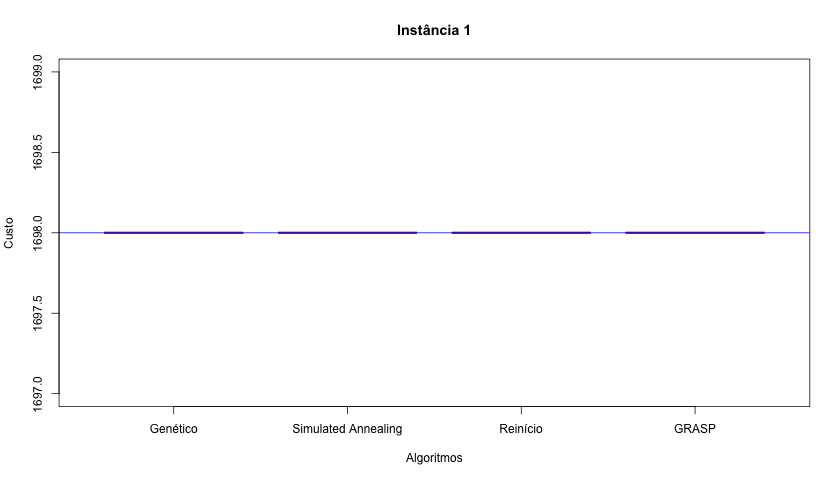
\includegraphics[width=1\linewidth]{img/1.png}
				\caption{BoxPlot da Instância \textit{a05100}.}
				\label{fig:a05100}
			\end{figure}
	
		\subsubsection{Instância \textit{a05200}}
			\begin{figure}[H]
				\centering
				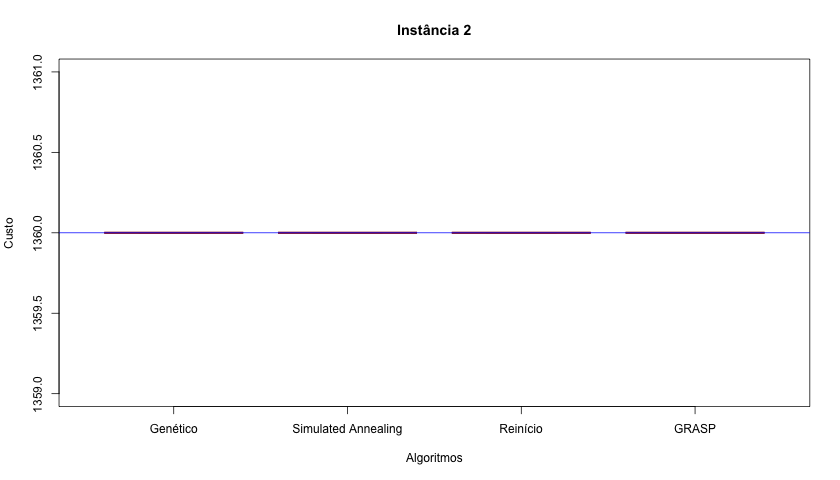
\includegraphics[width=1\linewidth]{img/2.png}
				\caption{BoxPlot da Instância \textit{a05200}.}
				\label{fig:a05200}
			\end{figure}
	
		\subsubsection{Instância \textit{a10100}}
			\begin{figure}[H]
				\centering
				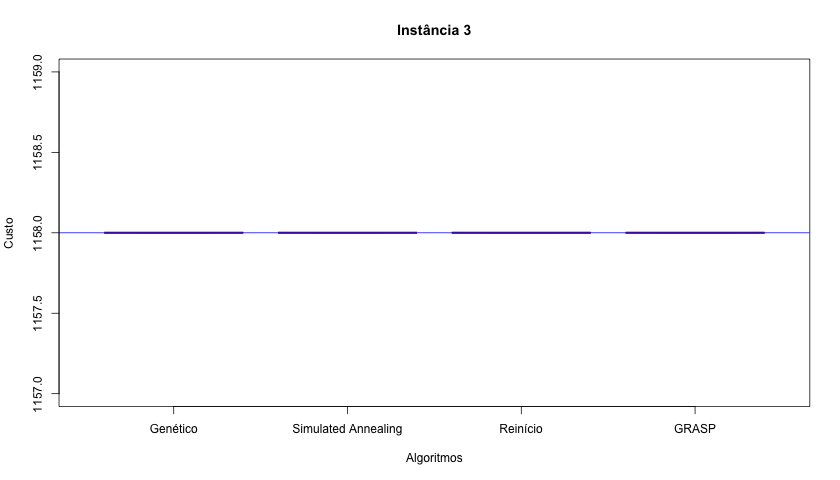
\includegraphics[width=1\linewidth]{img/3.png}
				\caption{BoxPlot da Instância \textit{a10100}.}
				\label{fig:a10100}
			\end{figure}
	
		\subsubsection{Instância \textit{a10200}}
			\begin{figure}[H]
				\centering
				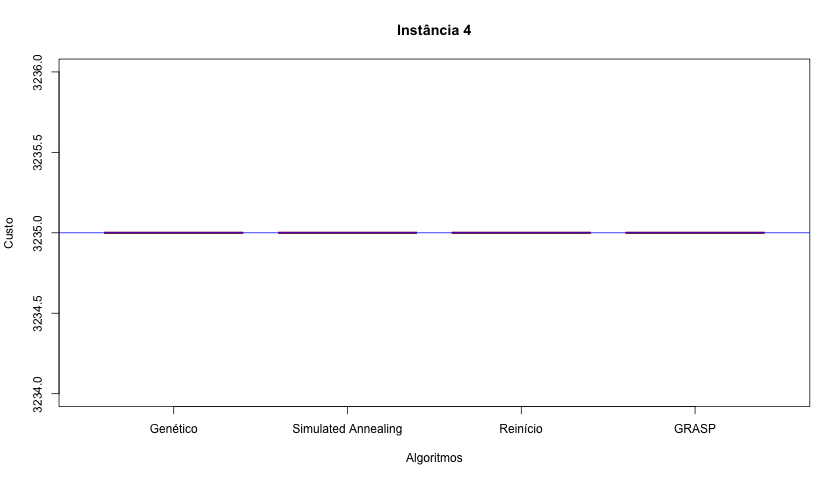
\includegraphics[width=1\linewidth]{img/4.png}
				\caption{BoxPlot da Instância \textit{a10200}.}
				\label{fig:a10200}
			\end{figure}
	
		\subsubsection{Instância \textit{a20100}}
			\begin{figure}[H]
				\centering
				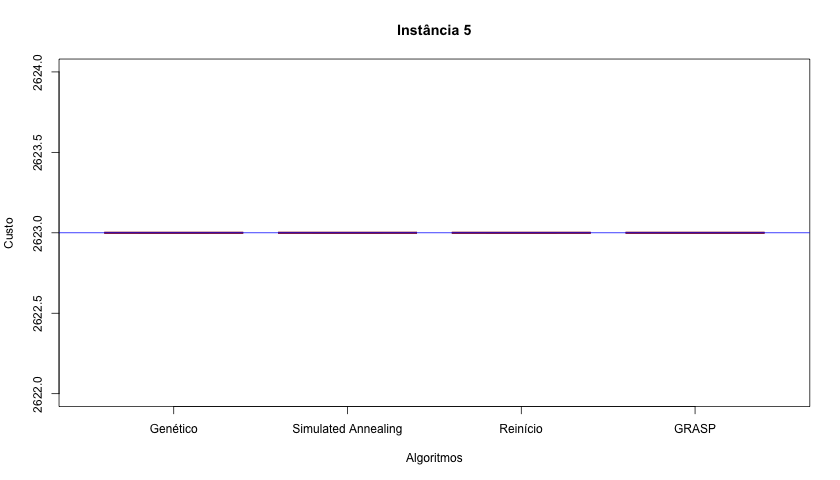
\includegraphics[width=1\linewidth]{img/5.png}
				\caption{BoxPlot da Instância \textit{a20100}.}
				\label{fig:a20100}
			\end{figure}
	
		\subsubsection{Instância \textit{a20200}}
			\begin{figure}[H]
				\centering
				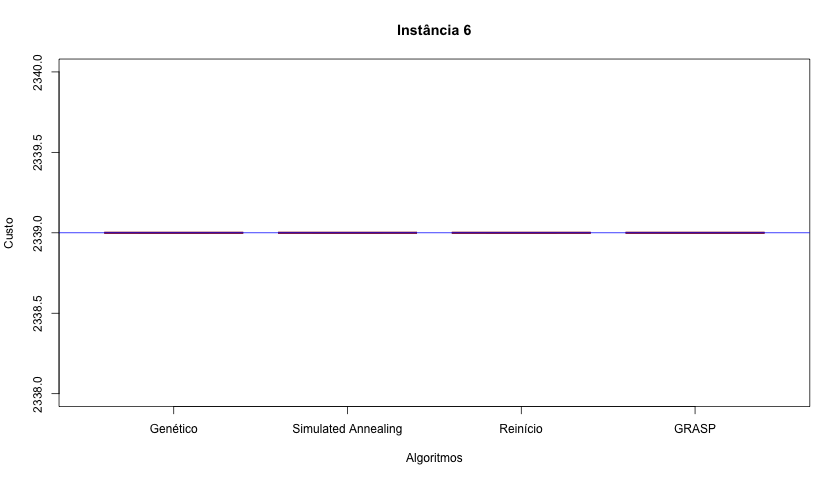
\includegraphics[width=1\linewidth]{img/6.png}
				\caption{BoxPlot da Instância \textit{a20200}.}
				\label{fig:a20200}
			\end{figure}
	

	
		\subsubsection{Instância \textit{c05100}}
			\begin{figure}[H]
				\centering
				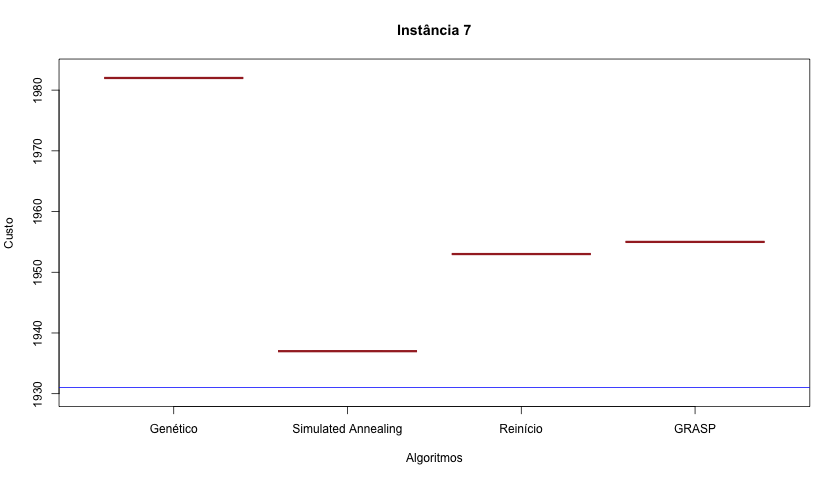
\includegraphics[width=1\linewidth]{img/7.png}
				\caption{BoxPlot da Instância \textit{c05100}.}
				\label{fig:c05100}
			\end{figure}
	
		\subsubsection{Instância \textit{c05200}}
			\begin{figure}[H]
				\centering
				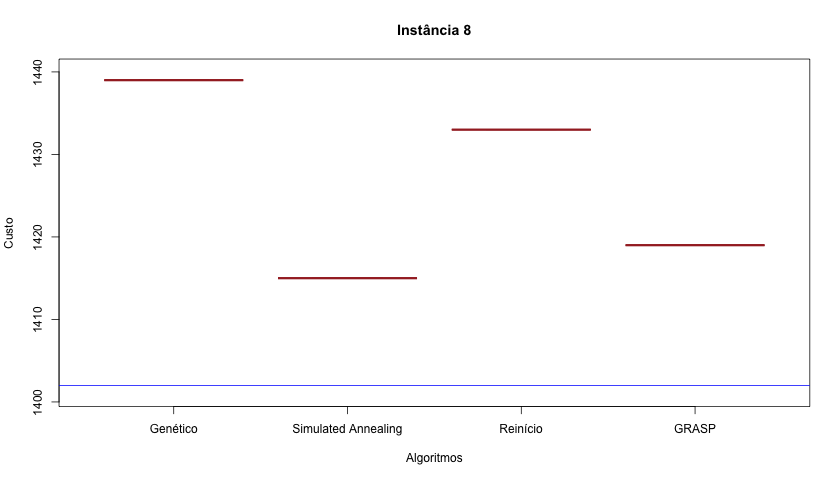
\includegraphics[width=1\linewidth]{img/8.png}
				\caption{BoxPlot da Instância \textit{c05200}.}
				\label{fig:c05200}
			\end{figure}
	
		\subsubsection{Instância \textit{c10100}}
			\begin{figure}[H]
				\centering
				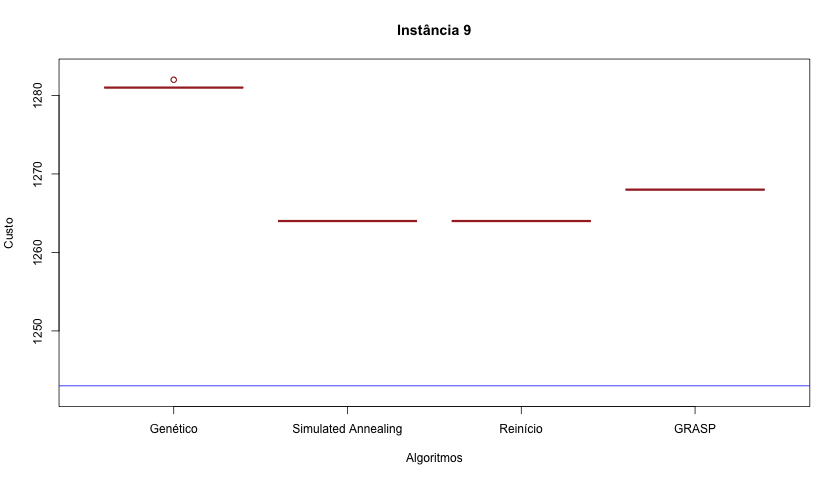
\includegraphics[width=1\linewidth]{img/9.png}
				\caption{BoxPlot da Instância \textit{c10100}.}
				\label{fig:c10100}
			\end{figure}
	
		\subsubsection{Instância \textit{c10200}}
			\begin{figure}[H]
				\centering
				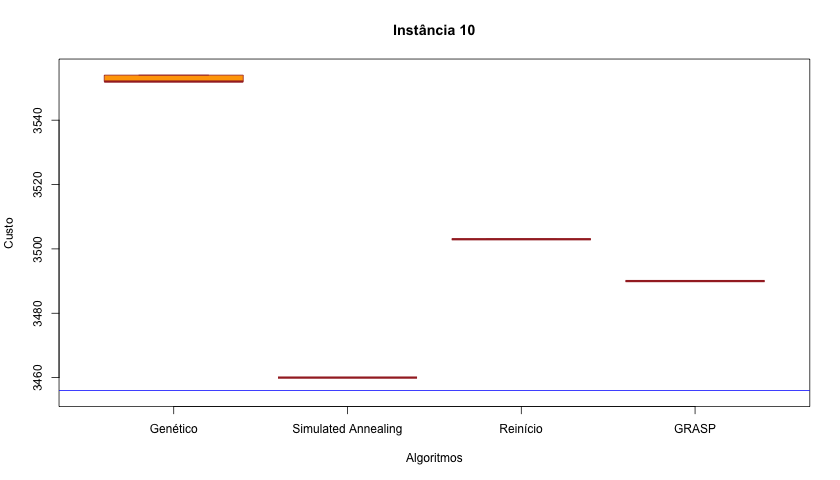
\includegraphics[width=1\linewidth]{img/10.png}
				\caption{BoxPlot da Instância \textit{c10200}.}
				\label{fig:c10200}
			\end{figure}
	
		\subsubsection{Instância \textit{c20100}}
			\begin{figure}[H]
				\centering
				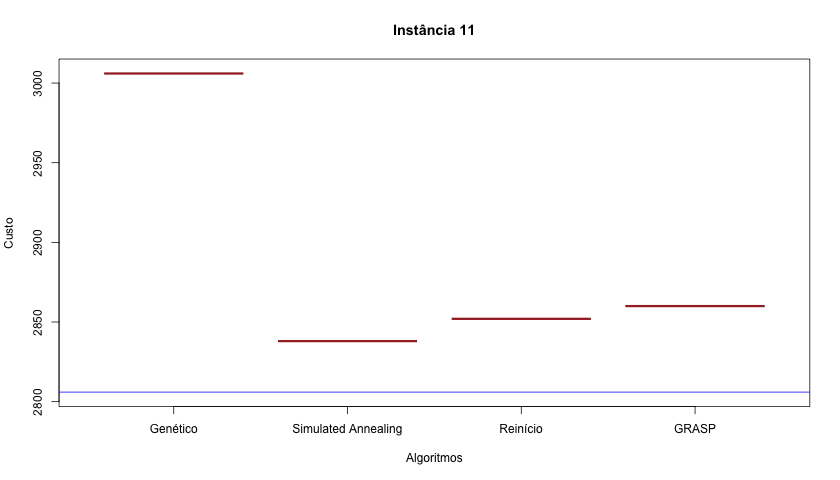
\includegraphics[width=1\linewidth]{img/11.png}
				\caption{BoxPlot da Instância \textit{c20100}.}
				\label{fig:c20100}
			\end{figure}
	
		\subsubsection{Instância \textit{c20200}}
			\begin{figure}[H]
				\centering
				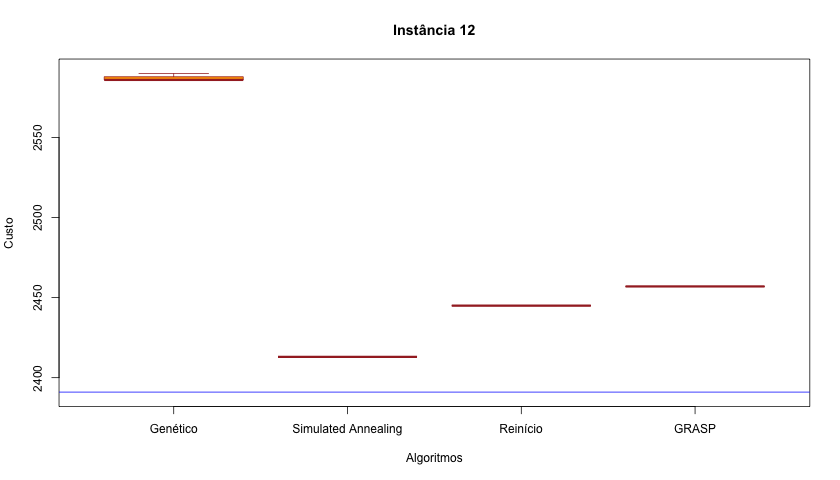
\includegraphics[width=1\linewidth]{img/12.png}
				\caption{BoxPlot da Instância \textit{c20200}.}
				\label{fig:c20200}
			\end{figure}


	
		\subsubsection{Instância \textit{e05100}}
			\begin{figure}[H]
				\centering
				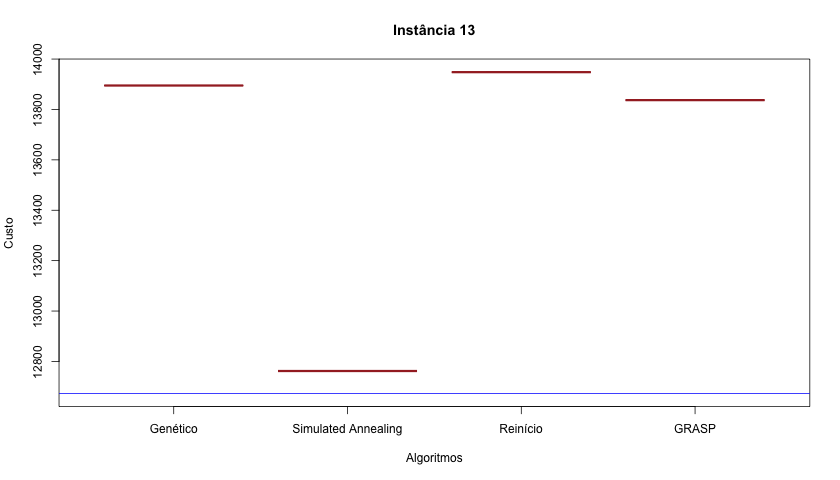
\includegraphics[width=1\linewidth]{img/13.png}
				\caption{BoxPlot da Instância \textit{e05100}.}
				\label{fig:e05100}
			\end{figure}
	
		\subsubsection{Instância \textit{e05200}}
			\begin{figure}[H]
				\centering
				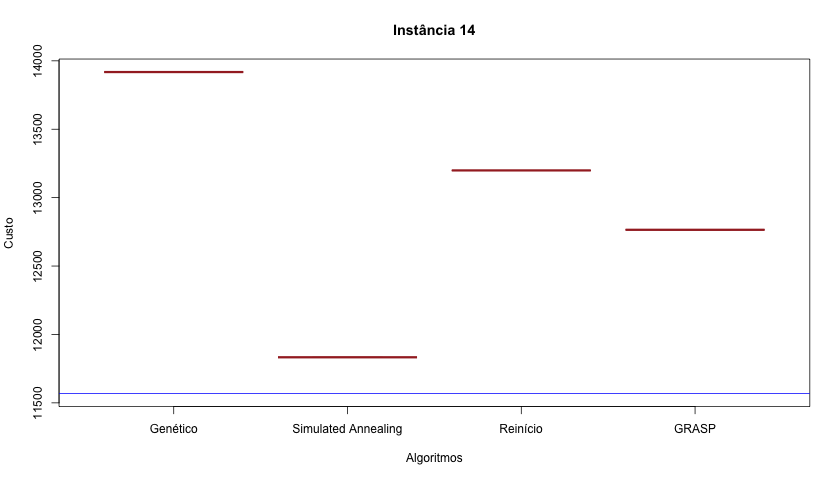
\includegraphics[width=1\linewidth]{img/14.png}
				\caption{BoxPlot da Instância \textit{e05200}.}
				\label{fig:e05200}
			\end{figure}
	
		\subsubsection{Instância \textit{e10100}}
			\begin{figure}[H]
				\centering
				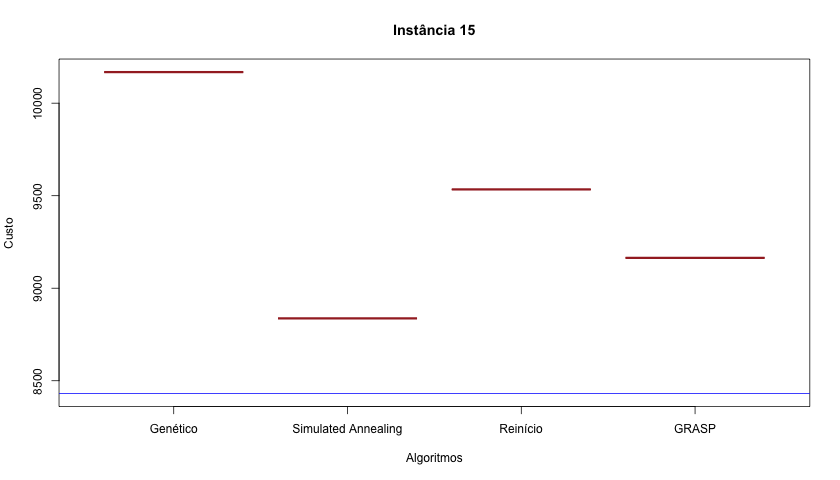
\includegraphics[width=1\linewidth]{img/15.png}
				\caption{BoxPlot da Instância \textit{e10100}.}
				\label{fig:e10100}
			\end{figure}
	
		\subsubsection{Instância \textit{e10200}}
			\begin{figure}[H]
				\centering
				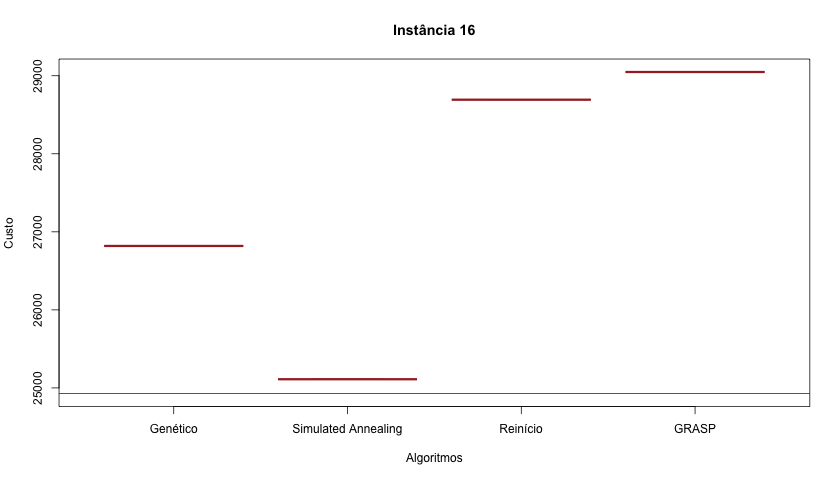
\includegraphics[width=1\linewidth]{img/16.png}
				\caption{BoxPlot da Instância \textit{e10200}.}
				\label{fig:e10200}
			\end{figure}
	
		\subsubsection{Instância \textit{e20100}}
			\begin{figure}[H]
				\centering
				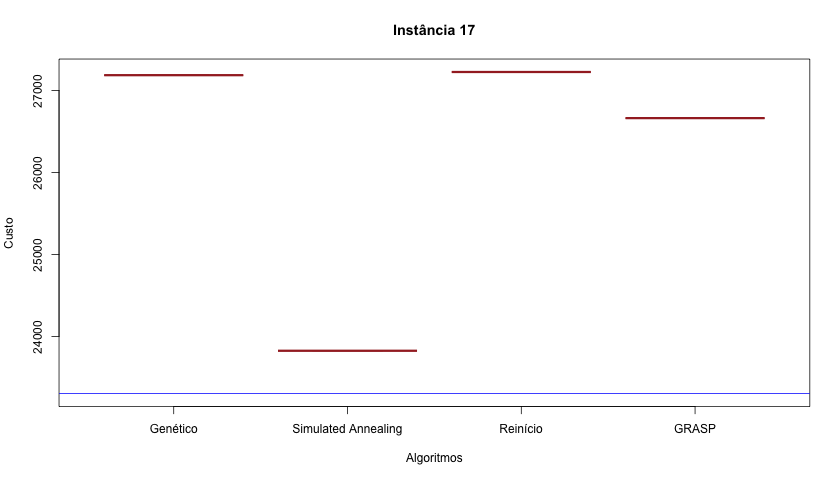
\includegraphics[width=1\linewidth]{img/17.png}
				\caption{BoxPlot da Instância \textit{e20100}.}
				\label{fig:e20100}
			\end{figure}
	
		\subsubsection{Instância \textit{e20200}}
			\begin{figure}[H]
				\centering
				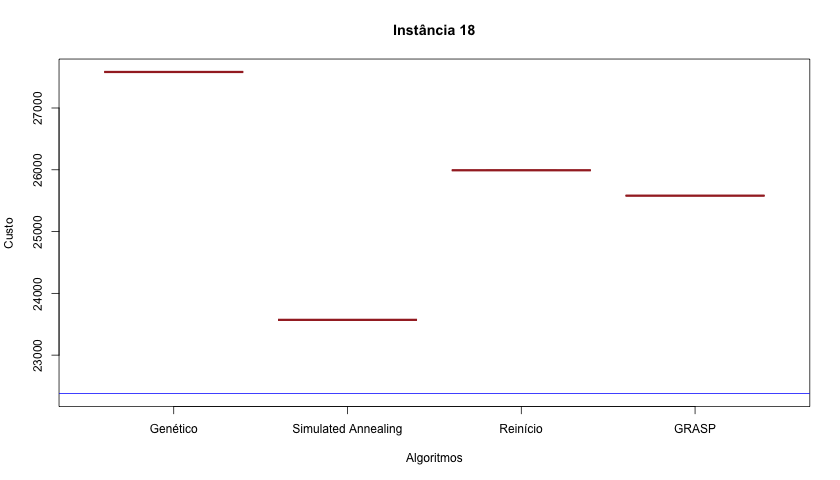
\includegraphics[width=1\linewidth]{img/18.png}
				\caption{BoxPlot da Instância \textit{e20200}.}
				\label{fig:e20200}
			\end{figure}
			
	
	\subsection{Estudo Estatísticos}
		Como análise comparativa final, foi confeccionado uma tabela comparando a média das distância de todos os algoritmos em todas as instâncias executadas. O resultado é exibido na Tabela \ref{tab:comparacaoFinal}.
		
	\begin{table}[h]
		\caption{Análise final de proximidade de cada algoritmo em relação ao ótimo.} \label{tab:comparacaoFinal}
		\centering
	    \begin{tabular}{c|c}
	    \hline
	    \textbf{Algoritmos}  &  \textbf{Média Geral em Relação ao Ótimo} \\ \hline \hline
	    Algoritmo Genético   &  94.00048 \%                \\
	    Recozimento Simulado &  98.85725 \%                \\
	    Método Reinício      &  95.29829 \%                \\
	    GRASP                &  95.83031 \%                \\ \hline
	    \end{tabular}
	\end{table}
	
	É possível concluir que todos os algoritmos teve um resultado médio acima de 94\% em todas as instâncias, sendo uma boa porcentagem quando necessita-se de um valor próximo ao ótimo em problemas combinatórios.
	
	Um item que deve-se atentar é no algoritmo de Recozimento Simulado que obteve uma média geral de quase 99\% de proximidade ao ótimo global encontrado pela literatura.
	

%%%%%%%%%%%%%%%%%%%%%%%%%%%%%%%%%%%%%%%%%%%%%%%%%%%%%%%%%%%%%%%%%%%%%%%%%%%%%%%%%%%%%%%%%%%%%%%%
%                                                                                              %
%                                           Conclusão                                         %
%                                                                                              %
%%%%%%%%%%%%%%%%%%%%%%%%%%%%%%%%%%%%%%%%%%%%%%%%%%%%%%%%%%%%%%%%%%%%%%%%%%%%%%%%%%%%%%%%%%%%%%%

\section{Comentários Finais}\label{sec:figs}
	A primeira conclusão a ser feita é a diferença do Algoritmo Genético em relação aos outros. Diferentemente do Genético, os três algoritmos compartilham da mesma natureza de procura que é baseada na geração de indivíduos aleatórios e busca local em seus vizinhos o que implica exatamente nos dados amostrados. Os três outros algoritmos (Recozimento Simulado, Método de Reinício e GRASP) utilizam de um processamento simples. Com não é necessário realizar muitas operações para completar uma iteração de seu processamento, eles permitem que sejam realizados mais cálculos por intervalo de tempo, proporcionando uma vantagem maior quando o processador de testes consegue realizar muito processamento por segundo. Estes algoritmos, nesta vantagem, permitem que vasculhem uma gama maior de locais a procura de um ótimo/solução boa favorável, o que realmente acontece. Ao contrário, o Algoritmo Genético é um algoritmo lento e com curva de otimização lenta já que é preciso realizar várias operações em seu processamento.
	
	Um item importante a ser abordado é o método de avaliação presente nos métodos \verb|Avalia_Solucao()| e \verb|Gera_Vizinho()|. Como o método possui duas funções diferentes (uma pra soluções válidas e outra para inválidas), é possível perceber que resultados válidos/factíveis são gerados de forma mais rápida tornando o algoritmo mais eficaz. O método \verb|Avalia_Solucao()| é invocado somente na construção de uma solução incial aleatória nos algoritmos Recozimento Simulado, Método de Reinício e GRASP melhorando ainda mais sua performance ao utilizar o procedimento de geração de vizinho otimizada (no qual não necessita de invocar o método de avaliação).
	
	Os parâmetros de todos os algoritmos foram mantidos os mesmos para todas as instâncias para generalizar seu desempenho e eficiência na procura de boas soluções sem depender de determinadas características específicas de determinada instância.

	Também foi possível concluir que a literatura utiliza um tempo maior de execução para encontrar soluções ótimas, o que difere deste trabalho. Neste, foi determinado um tempo de um minuto por execução o que restringe ainda mais a proximidade do ótimo global. Entretanto, todos os algoritmos obtiveram excelente resultados mesmo em tempo de execução curto.
	
	
\section{Código dos Algoritmos}
	Os algoritmos \textit{Shell Script}, \textit{Backtracking}, \textit{Branch and Bound 1} e \textit{Branch and Bound 2} estão distribuídos nas páginas \pageref{cod:shell}, \pageref{cod:bt}, \pageref{cod:bb1} e \pageref{cod:bb1} respectivamente.
	\subsection{\textit{Shell Script}} \label{cod:shell}

\begin{minted}
[
frame=lines,
framesep=2mm,
tabsize=3,
breaklines=true,
baselinestretch=1.2,
linenos,
fontsize=\footnotesize
]{shell}
#!/bin/bash

echo "Quantas iteracoes?"
read quantidade_iteracoes;
echo

eval "rm algori*"
eval "gcc n-Queens-Prize-Backtracking/n-queens-prize-backtracking.c -Ofast -o n-Queens-Prize-Backtracking/n-Queens-Prize-Backtracking"
eval "gcc n-Queens-Prize-BranchAndBound-1/n-queens-prize-branchAndBound-1.c -Ofast -o n-Queens-Prize-BranchAndBound-1/n-Queens-Prize-BranchAndBound-1"
eval "gcc n-Queens-Prize-BranchAndBound-2/n-queens-prize-branchAndBound-2.c -Ofast -o n-Queens-Prize-BranchAndBound-2/n-Queens-Prize-BranchAndBound-2"

instancias=( nqp005.txt nqp008.txt nqp010.txt nqp020.txt nqp030.txt nqp040.txt nqp050.txt nqp060.txt nqp070.txt nqp080.txt nqp090.txt nqp100.txt nqp200.txt )

algoritmos=( n-Queens-Prize-Backtracking n-Queens-Prize-BranchAndBound-1 n-Queens-Prize-BranchAndBound-2 )

for algoritmo in "${algoritmos[@]}"
do
	echo $algoritmo

	for instancia in "${instancias[@]}"
	do
		echo $instancia

		for (( i = 0; i < "$quantidade_iteracoes"; i++ )); do
			echo "$i"

			cmd="./$algoritmo/$algoritmo $instancia $i*1234 60 0"
			date
			echo $cmd
			$cmd
		done
		echo

	done
	echo

done

\end{minted}

	\subsection{\textit{Backtracking}} \label{cod:bt}



\begin{minted}
[
frame=lines,
framesep=2mm,
tabsize=3,
breaklines=true,
baselinestretch=1.2,
linenos,
fontsize=\footnotesize
]{c}
#include <stdio.h>
#include <stdlib.h>
#include <time.h>

// variável global sobre a quantidade de colunas/linhas da matriz
int global_tamanho_matriz = -1;
// variável que ativa impressoes na tela
char global_imprime_tela_ativado = 0;

// Variáveis de tempo para cálculo do intervalo de tempo de execução
time_t endwait, start;


/*
 * Estrutura que representa um tabuleiro.
 *
 * Um ponteiro para um vetor de onde representa cada posicao da rainha na coluna
 * O valor de prêmrio do tabuleiro no estado atual
 */
typedef struct Struct_Tabuleiro {
	int * colunas;
	int   premio;
} Tabuleiro;


/*
 * Estrutura de representação de Fila
 *
 * Esta fila é utilizada para organizar a ordem de seleção das rainhas
 */
typedef struct Struct_Fila {
	int           lugar; // Posição da rainha
	struct Struct_Fila * proximo;
} Fila;



/*
 * Procedimento que verifica se a fila passada por parâmetro está vazia.
 *
 * Retorna valores boleanos
 */
char Fila_Esta_Vazia(Fila * f) {
	if (f == NULL) {
		return 1;
	} else
		return 0;
}



/*
 * Procedimento que adiciona um novo valor à fila
 */
void Enfilera(Fila ** f, int l) {
	Fila * atual = 0, * novo = 0;

	// Cria um novo nó e adiciona informações
	novo = calloc(1, sizeof(Fila));
	novo->lugar = l;
	novo->proximo = NULL;


	// Se a fila estiver vazia, coloca na cabeça
	if (Fila_Esta_Vazia(*f)) {

		* f = novo;

	} else {
		// Caso contrário, coloca na calda

		atual = * f;

		while(atual->proximo != NULL) {
			atual = atual->proximo;
		}

		atual->proximo = novo;
	}
}



/*
 * Procedimento que realiza a retirada de um elemento da fila seguindo sua natureza
 */
int Desenfilera(Fila ** f) {
	Fila * retirar = 0, * fila = * f;
	int posicao = 0;

	// Se a fila estiver vazia, informa erro e termina o programa
	if (Fila_Esta_Vazia(*f)) {
		printf("\n\n[ERRO] Impossível retirar de uma fila vazia. \tFinalizando o programa.");
		return -1;
	} else {
		// caso contrário, retira o primeiro elemento.
		posicao = fila->lugar;
		retirar = fila;

		fila = fila->proximo;

		free(retirar);

		*f = fila;

		return posicao;
	}
}



/*
 * Procedimento que realiza o processo de retirar todos os elementos da fila
 */
void Desaloca_Fila(Fila ** f) {
	Fila * retirar = 0;

	// Retira todos os elementos da fila
	while (*f != NULL) {
		retirar = *f;

		*f = (*f)->proximo;

		free (retirar);
	}

}



/*
 * Procedimento para impressão da Fila na tela
 */
void Imprime_Fila(Fila * f) {
	Fila * atual = f;

	if (global_imprime_tela_ativado) {

		printf("\n\n\t\t");
		while (atual != NULL) {
			printf("%d -> ", atual->lugar);
			atual = atual->proximo;
		}
		printf("NULL");

		fflush(stdout);
	}
}



/*
 * Procedimento responsável por gerar uma fila de posições de rainhas em ordem aleatória.
 *
 * Primeiro cria-se um vetor com os valores de 1..n ordenado simbolizando a ordem das rainhas.
 * Em seguida, é gerado dois valores inteiros posicao1 e posicao2 de forma aleatória e estes
 *		são utilizados para a comutação dos valores situados em vetor[posicao1] e vetor[posicao2]
 * No final de algumas iterações, estes respectivos valores já desordenados são copiados para
 *		a fila para que o algoritmo use.
 */
Fila * Cria_Fila_Aleatoria() {
	Fila * f = 0, * cabeca = 0;

	int vetor_valores_fila [global_tamanho_matriz],
			i = 0,
			permutacoes = global_tamanho_matriz * 10,
			posicao1 = 0, posicao2 = 0, temp = 0;

	// Cria-se um vetor com valores ordenados de 1..n_rainhas
	for (i = 0; i < global_tamanho_matriz; i++) {
		vetor_valores_fila[i] = i;
	}

	// Realiza várias permutações dos valores deste vetor de acordo com os dois índices gerados
		// Realiza-se global_tamanho_matriz * 10 permutações
	i = 0;
	while (i < permutacoes) {
		// Gera primeiro índice
		posicao1 = rand() % global_tamanho_matriz;

		// Gera segundo índice
		posicao2 = rand() % global_tamanho_matriz;

		// Realiza a comutação dos valores dos respectivos índices
		temp = vetor_valores_fila[posicao1];
		vetor_valores_fila[posicao1] = vetor_valores_fila[posicao2];
		vetor_valores_fila[posicao2] = temp;

		i++;
	}

	// Aloca a fila e adiciona os valores após realizar a desordem
	cabeca = calloc(1, sizeof(Fila));

	f = cabeca;

	// Copia os valores do vetor para a fila
	i = 0;
	while (i < global_tamanho_matriz - 1) {

		f->lugar = vetor_valores_fila[i];

		f->proximo = calloc(1, sizeof(Fila));

		f = f->proximo;

		i++;
	}

	f->lugar = vetor_valores_fila[i];

	f->proximo = NULL;

	// Retorna a fila desordenada
	return cabeca;
}



/*
 * Procedimento para retorndo do de prêmio específico de uma célula
 */
int Retorna_Premio(int * premios, int linha, int coluna) {

	// Acessa o vetor como se fosse uma matriz comum nxn.
	return premios[linha * global_tamanho_matriz + coluna];
}



/*
 * Procedimento para realizar a leitura dos arquivo prêmio
 *
 * Este também armazena o maior premio lido e o retorna.
 */
void Le_Premios(char * diretorio, int ** premios){
	FILE * file = 0;
	int i = 0;
	int premio_lido = 0;
	int quantidade_celulas = 0;

	// Abre o arquivo de prêmios em forma de leitura
	file = fopen(diretorio, "r");

	// Verifica se a abertura foi feita com sucesso
	if (file != NULL) {

		//lê a primeira informação (quantas linhas existem)
		fscanf(file, "%d", &global_tamanho_matriz);
		if (global_imprime_tela_ativado)
			printf("\n[INFO] Quantidade de colunas do tabuleiro = %d.\n", global_tamanho_matriz);

		// Se o valor de tamanho da matriz for um valor válido
		if (global_tamanho_matriz > 0) {

			quantidade_celulas = global_tamanho_matriz * global_tamanho_matriz;

			// Aloca a matriz de prêmios
			* premios = calloc(quantidade_celulas, sizeof(int));

			// Começa a coleta dos prêmios
			fscanf(file, "%d", &premio_lido);

			// Salvas os prêmios e coleta o próximo
			while(i < quantidade_celulas) {

				if (global_imprime_tela_ativado) {
					// Imprime na tela o prêmio lido
					printf("\n[INFO] Lendo premio [%d,%d] = %d.", i / global_tamanho_matriz + 1, i % global_tamanho_matriz + 1, premio_lido);
					fflush(stdout);
				}

				// Salva no vetor
				(*premios)[i++] = premio_lido;

				// Lê o próximo prêmio
				fscanf(file, "%d", &premio_lido);
			}
		} else {
			// Informa Erro
			printf("\n[ERRO] Quantidade de rainhas insuficiente!\n\n");
			exit(-1);
		}

		// Fecho o arquivo
		fclose(file);
	}
	else {
		// Informa Erro
		printf("\n[ERRO] Falha na leitura do arquivo de configuração!\n\n");
		exit(-1);
	}
}



/*
 * Como utiliza-se uma estrutura fila com todas as opções e sem repetição, não
 *		existe a possibilidade de duas rainhas ficarem numa mesma linha
 *		vertical, horizontal (isso pois os valores não se repetem).
 *
 * Com isso, basta verificar se as diagonais estão conflitando.
 */
char Posicao_Eh_Valida(Tabuleiro t, int col, int pos) {
	int i = 0;
	char esquerda_diagonal = 0, direita_diagonal = 0;

	// Inicializa dizendo que as diagonais não estão ocupadas
	esquerda_diagonal = direita_diagonal = 1;

	// Da posição da rainha até a coluna 0, faça:
	i = col;
	while (i > 0) {

		// Verifica:
		//		Diagonal esquerda-direita
		if (t.colunas[col - i]  == pos + i) {
			esquerda_diagonal = 0;

		// Verifica:
		//		Diagonal direita-esquerda
		} else
			if (t.colunas[col - i] == pos - i) {
			direita_diagonal = 0;
		}

		// Verifica validade
		// Caso alguma diagonal já esteja ocupada, aborta o procedimento
			// informando que esta posição é inválida
		if (esquerda_diagonal == 0 || direita_diagonal == 0) {
			return 0;
		}

		i--;
	}

	// Verifica validade das diagonais
	if (esquerda_diagonal == 1 && direita_diagonal == 1)
		return 1;
	else
		return 0;
}



/*
 * Procedimento que copia os dados de um tabuleiro para outro.
 *
 * Este procedimento é utilizando quando encontra-se um novo valor de prêmio maior
 *		que o atual e assim, realiza-se a substituição do tabuleiro antigo pelo novo
 *		encontrado.
 */
void Copia_Novo_Tabuleiro(Tabuleiro tabuleiro_atual, Tabuleiro * tabuleiro_maior) {
	int i = 0;

	tabuleiro_maior->premio           = tabuleiro_atual.premio;

	for (i = 0; i < global_tamanho_matriz; i++) {
		tabuleiro_maior->colunas[i]   = tabuleiro_atual.colunas[i];
	}
}



/*
 * Procedimento que adiciona uma nova rainha no tabuleiro já calculando o prêmio desta.
 *
 * Este procedimento não precisa verificar a validade da posição já que este já foi calculado
 *		quando a rainha foi selecionada.
 */
void Adiciona_Rainha_Tabuleiro_Calculando_Premio(Tabuleiro * t, int posicao,  int r, int * premios) {

	t->premio += Retorna_Premio(premios, r, posicao);
	t->colunas[posicao] = r;
}



/*
 * Procedimento que retira a rainha do tabuleiro calculando o novo prêmio
 */
void Retira_Rainha_Tabuleiro_Calculando_Premio(Tabuleiro * t, int posicao, int r, int * premios) {
	t->premio -= Retorna_Premio(premios, r, posicao);
	t->colunas[posicao] = -1;
}



/*
 * Procedimento que inicializa um novo tabuleiro
 */
Tabuleiro * Cria_Tabuleiro(){
	int i = 0;
	Tabuleiro * t = 0;

	t = calloc(1, sizeof(Tabuleiro));
	t->colunas = calloc(global_tamanho_matriz, sizeof(int));

	for (i = 0; i < global_tamanho_matriz; i++)
		t->colunas[i] = -1;

	return t;
}



/*
 * Procedimento que imprime o tabuleiro junto com os prêmios
 */
void Imprime_Tabuleiro (Tabuleiro t, Tabuleiro maior, int * premios) {
	int i = 0, j = 0;

	if (global_imprime_tela_ativado) {

		printf("\n");

		for (i = 0; i < global_tamanho_matriz; i++) {
				printf("\n\t");
			for (j = 0; j < global_tamanho_matriz * 2; j++) {
				if ( j < global_tamanho_matriz) {
					if (i == t.colunas[j])
						printf("%3d ", i);
					else
						printf(" -1 ");
				}
				else {
					if (j == global_tamanho_matriz)
						printf("\t\t");
					printf("%3d ", premios[i * global_tamanho_matriz + j - global_tamanho_matriz]);
				}

			}

			fflush(stdout);
		}

		printf("\tPremio_Atual: %d;\tMaior_Premio: %d.", t.premio, maior.premio);

		fflush(stdout);
	}
}


/*
 * Procedimento que imprime o tabuleiro, junto com os prêmios informando fim da execução
 */
void Imprime_Tabuleiro_Final (Tabuleiro maior, int * premios) {
	int i = 0, j = 0;
	FILE * saida = 0;

	if (global_imprime_tela_ativado) {

		printf("\n\n[INFO] Resultado Final do Processamento:");

		for (i = 0; i < global_tamanho_matriz; i++) {
				printf("\n\t");
			for (j = 0; j < global_tamanho_matriz * 2; j++) {
				if ( j < global_tamanho_matriz) {
					if (i == maior.colunas[j])
						printf("%3d ", i);
					else
						printf(" -1 ");
				}
				else {
					if (j == global_tamanho_matriz)
						printf("\t\t");
					printf("%3d ", premios[i * global_tamanho_matriz + j - global_tamanho_matriz]);
				}
			}

			fflush(stdout);
		}

		printf("\tPremio: %d.",maior.premio);
		printf("\n[INFO] Resultado Final do Processamento.\n");
	} else {
		saida = fopen("algoritmo0.txt", "a");

		if (saida) {
			fprintf(saida, "%d\n", maior.premio);
		}

		fclose(saida);
	}

	fflush(stdout);
}



/*
 * Procedimento que libera memória
 */
 void Desaloca_Tabuleiro (Tabuleiro ** f) {
	if (*f != 0) {
		free((*f)->colunas);
		free(*f);
	}
 }



/*
 * Procedimento que libera memória
 */
void Desaloca_Premios (int ** premios) {
	if (*premios != 0)
		free(*premios);
}



/*
 * Método de branch and bound desenvolvido
 */
void n_Rainhas_Prize(int coluna_atual, Tabuleiro * tabuleiro_atual, Tabuleiro * tabuleiro_maior, Fila ** posicoes_restantes, int * premios) {
	int iteracoes = 0, linha_atual_temp = 0;

	// Recebe o tempo atual.
	start = time(NULL);

	// Verifica se o tempo excedeu o liminte estabelecido.
	if (start > endwait) {
		// Se sim, cancela totalmente a continuação da recursão
		return ;
	}


	// Varre a fila com os valores que sobraram
		// A cada recursão, um item é retirado

	// Caso tenha percorrido todas as rainhas deste contexto de recursão,
		// o while será impedido de ser executando forçando a realizar o
		// retorno à um nível acima de recursao
	while (iteracoes < global_tamanho_matriz - coluna_atual) {

		Imprime_Fila(* posicoes_restantes);
		Imprime_Tabuleiro(*tabuleiro_atual, *tabuleiro_maior, premios);

		// Retira um item da fila e salva numa variável local
		linha_atual_temp = Desenfilera( posicoes_restantes );

			printf("\nALERTA%d\n", linha_atual_temp);
		if (linha_atual_temp == -1) {
			Desaloca_Premios(&premios);

			Desaloca_Tabuleiro(&tabuleiro_maior);
			Desaloca_Tabuleiro(&tabuleiro_atual);
			exit(-1);
		}

		Imprime_Fila(* posicoes_restantes);
		if (global_imprime_tela_ativado) {
			printf("\t\tBuffer_Atual: %d", linha_atual_temp);
			fflush(stdout);
		}


		// Testa a validade da rainha retirada no momento
			// Se for posição válida realizará o processamento desta
			// Caso contrário, ela será posta no final da fila=
		if(Posicao_Eh_Valida(*tabuleiro_atual, coluna_atual, linha_atual_temp)) {

			// Adiciona a rainha no tabuleiro calculando o prêmio com sua inclusão
			Adiciona_Rainha_Tabuleiro_Calculando_Premio(tabuleiro_atual, coluna_atual, linha_atual_temp, premios);

			Imprime_Tabuleiro(*tabuleiro_atual, *tabuleiro_maior, premios);


			// Se a fila estiver vazia, significa que acabou de ser gerado uma solução
				// válida.
			// Assim, será verificado se o prêmio é melhor que o atual.
			if (Fila_Esta_Vazia(* posicoes_restantes)) {

				if (tabuleiro_atual->premio > tabuleiro_maior->premio) {

					if (global_imprime_tela_ativado)
						printf("\n\n[INFO] Novo Recorde Encontrado!");
					Copia_Novo_Tabuleiro(*tabuleiro_atual, tabuleiro_maior);

					Imprime_Tabuleiro(*tabuleiro_atual, *tabuleiro_maior, premios);
				}


				Imprime_Fila(*posicoes_restantes);

				// Após chegar na folha, a recursão é revertida até que encontre
					// uma próxima solução pra explorar.
				Enfilera(posicoes_restantes, linha_atual_temp);

				Imprime_Fila(*posicoes_restantes);

				// Como mencionado, a raínha é posta novamente na fila para a procura
					// de novas soluções
				Retira_Rainha_Tabuleiro_Calculando_Premio(tabuleiro_atual, coluna_atual, linha_atual_temp, premios);


				return ;


			// Se não for a última rainha, então realiza as análises de bound
			} else {

				n_Rainhas_Prize(coluna_atual + 1, tabuleiro_atual, tabuleiro_maior, posicoes_restantes, premios);


				Enfilera(posicoes_restantes, linha_atual_temp);

				Retira_Rainha_Tabuleiro_Calculando_Premio(tabuleiro_atual, coluna_atual, linha_atual_temp, premios);

				Imprime_Fila(*posicoes_restantes);

				iteracoes++;
			} // if


		// Se a posição escolhida não for válida
		} else {

			if(global_imprime_tela_ativado) {
				printf("\n[INFO] Posição Inválida. Retornando o valor %d à fila", linha_atual_temp);
				fflush(stdout);
			}

			// Readiciona-la no final da fila
			Enfilera(posicoes_restantes, linha_atual_temp);

			Imprime_Fila(*posicoes_restantes);

			// Passa pra próxima rainha
			iteracoes++;

		} // if

	} // While


	// Após ter percorrido todos as soluções deste nível e seus subníveis
		// é retornado um nível para continuar a busca.

	if(global_imprime_tela_ativado)
		printf("\n[INFO] Saindo do nível %d", coluna_atual);

	return ;

}


int main(int argc, char** argv) {
	int * premios = 0;
	char * diretorio = 0;
	Tabuleiro * tabuleiro_atual = 0, * tabuleiro_maximo_encontrado = 0;
	Fila * fila_rainhas = 0;
	time_t seconds = 0;

	if (argc != 4) {
		diretorio = argv[1];
		srand(atoi(argv[2]));
		seconds = atoi(argv[3]);
		global_imprime_tela_ativado = atoi(argv[4]);

	} else {
		exit(-1);
	}

	Le_Premios(diretorio, &premios);

	tabuleiro_atual = Cria_Tabuleiro();
	tabuleiro_maximo_encontrado = Cria_Tabuleiro();

	fila_rainhas = Cria_Fila_Aleatoria();

	start = time(NULL);

	endwait = start + seconds;


	n_Rainhas_Prize(0, tabuleiro_atual, tabuleiro_maximo_encontrado, &fila_rainhas, premios);


	Imprime_Tabuleiro_Final(*tabuleiro_maximo_encontrado, premios);

	Desaloca_Fila(&fila_rainhas);
	Desaloca_Premios(&premios);
	Desaloca_Tabuleiro(&tabuleiro_maximo_encontrado);
	Desaloca_Tabuleiro(&tabuleiro_atual);

	return (EXIT_SUCCESS);
}

\end{minted}

	\subsection{\textit{Branch and Bound} 1} \label{cod:bb1}

\begin{minted}
[
frame=lines,
framesep=2mm,
tabsize=3,
breaklines=true,
baselinestretch=1.2,
linenos,
fontsize=\footnotesize
]{c}
#include <stdio.h>
#include <stdlib.h>
#include <time.h>

// variável global sobre a quantidade de colunas/linhas da matriz
int global_tamanho_matriz = -1;
// variável que ativa impressoes na tela
char global_imprime_tela_ativado = 0;

// Variáveis de tempo para cálculo do intervalo de tempo de execução
time_t endwait, start;


/*
 * Estrutura que representa um tabuleiro.
 *
 * Um ponteiro para um vetor de onde representa cada posicao da rainha na coluna
 * O valor de prêmrio do tabuleiro no estado atual
 */
typedef struct Struct_Tabuleiro {
	int * colunas;
	int   premio;
} Tabuleiro;


/*
 * Estrutura de representação de Fila
 *
 * Esta fila é utilizada para organizar a ordem de seleção das rainhas
 */
typedef struct Struct_Fila {
	int           lugar; // Posição da rainha
	struct Struct_Fila * proximo;
} Fila;



/*
 * Procedimento que verifica se a fila passada por parâmetro está vazia.
 *
 * Retorna valores boleanos
 */
char Fila_Esta_Vazia(Fila * f) {
	if (f == NULL) {
		return 1;
	} else
		return 0;
}



/*
 * Procedimento que adiciona um novo valor à fila
 */
void Enfilera(Fila ** f, int l) {
	Fila * atual = 0, * novo = 0;

	// Cria um novo nó e adiciona informações
	novo = calloc(1, sizeof(Fila));
	novo->lugar = l;
	novo->proximo = NULL;


	// Se a fila estiver vazia, coloca na cabeça
	if (Fila_Esta_Vazia(*f)) {

		* f = novo;

	} else {
		// Caso contrário, coloca na calda

		atual = * f;

		while(atual->proximo != NULL) {
			atual = atual->proximo;
		}

		atual->proximo = novo;
	}
}



/*
 * Procedimento que realiza a retirada de um elemento da fila seguindo sua natureza
 */
int Desenfilera(Fila ** f) {
	Fila * retirar = 0, * fila = * f;
	int posicao = 0;

	// Se a fila estiver vazia, informa erro e termina o programa
	if (Fila_Esta_Vazia(*f)) {
		printf("\n\n[ERRO] Impossível retirar de uma fila vazia.");
		return -1;

	} else {
		// caso contrário, retira o primeiro elemento.
		posicao = fila->lugar;
		retirar = fila;

		fila = fila->proximo;

		free(retirar);

		*f = fila;

		return posicao;
	}
}



/*
 * Procedimento que realiza o processo de retirar todos os elementos da fila
 */
void Desaloca_Fila(Fila * f) {
	Fila * retirar = 0;

	// Retira todos os elementos da fila
	while (f != NULL) {
		retirar = f;

		f = f->proximo;

		free (retirar);
	}

}



/*
 * Procedimento para impressão da Fila na tela
 */
void Imprime_Fila(Fila * f) {
	Fila * atual = f;

	if (global_imprime_tela_ativado) {

		printf("\n\n\t\t");
		while (atual != NULL) {
			printf("%d -> ", atual->lugar);
			atual = atual->proximo;
		}
		printf("NULL");

		fflush(stdout);
	}
}



/*
 * Procedimento responsável por gerar uma fila de posições de rainhas em ordem aleatória.
 *
 * Primeiro cria-se um vetor com os valores de 1..n ordenado simbolizando a ordem das rainhas.
 * Em seguida, é gerado dois valores inteiros posicao1 e posicao2 de forma aleatória e estes
 *		são utilizados para a comutação dos valores situados em vetor[posicao1] e vetor[posicao2]
 * No final de algumas iterações, estes respectivos valores já desordenados são copiados para
 *		a fila para que o algoritmo use.
 */
Fila * Cria_Fila_Aleatoria() {
	Fila * f = 0, * cabeca = 0;

	int vetor_valores_fila [global_tamanho_matriz],
			i = 0,
			permutacoes = global_tamanho_matriz * 10,
			posicao1 = 0, posicao2 = 0, temp = 0;

	// Cria-se um vetor com valores ordenados de 1..n_rainhas
	for (i = 0; i < global_tamanho_matriz; i++) {
		vetor_valores_fila[i] = i;
	}

	// Realiza várias permutações dos valores deste vetor de acordo com os dois índices gerados
		// Realiza-se global_tamanho_matriz * 10 permutações
	i = 0;
	while (i < permutacoes) {
		// Gera primeiro índice
		posicao1 = rand() % global_tamanho_matriz;

		// Gera segundo índice
		posicao2 = rand() % global_tamanho_matriz;

		// Realiza a comutação dos valores dos respectivos índices
		temp = vetor_valores_fila[posicao1];
		vetor_valores_fila[posicao1] = vetor_valores_fila[posicao2];
		vetor_valores_fila[posicao2] = temp;

		i++;
	}

	// Aloca a fila e adiciona os valores após realizar a desordem
	cabeca = calloc(1, sizeof(Fila));

	f = cabeca;

	// Copia os valores do vetor para a fila
	i = 0;
	while (i < global_tamanho_matriz - 1) {

		f->lugar = vetor_valores_fila[i];

		f->proximo = calloc(1, sizeof(Fila));

		f = f->proximo;

		i++;
	}

	f->lugar = vetor_valores_fila[i];

	f->proximo = NULL;

	// Retorna a fila desordenada
	return cabeca;
}



/*
 * Procedimento para retorndo do de prêmio específico de uma célula
 */
int Retorna_Premio(int * premios, int linha, int coluna) {

	// Acessa o vetor como se fosse uma matriz comum nxn.
	return premios[linha * global_tamanho_matriz + coluna];
}



/*
 * Procedimento para realizar a leitura dos arquivo prêmio
 *
 * Este também armazena o maior premio lido e o retorna.
 */
void Le_Premios(char * diretorio, int ** premios){
	FILE * file = 0;
	int i = 0;
	int premio_lido = 0;
	int quantidade_celulas = 0;

	// Abre o arquivo de prêmios em forma de leitura
	file = fopen(diretorio, "r");

	// Verifica se a abertura foi feita com sucesso
	if (file != NULL) {

		//lê a primeira informação (quantas linhas existem)
		fscanf(file, "%d", &global_tamanho_matriz);
		if (global_imprime_tela_ativado)
			printf("\n[INFO] Quantidade de colunas do tabuleiro = %d.\n", global_tamanho_matriz);

		// Se o valor de tamanho da matriz for um valor válido
		if (global_tamanho_matriz > 0) {

			quantidade_celulas = global_tamanho_matriz * global_tamanho_matriz;

			// Aloca a matriz de prêmios
			* premios = calloc(quantidade_celulas, sizeof(int));

			// Começa a coleta dos prêmios
			fscanf(file, "%d", &premio_lido);

			// Salvas os prêmios e coleta o próximo
			while(i < quantidade_celulas) {

				if (global_imprime_tela_ativado) {
					// Imprime na tela o prêmio lido
					printf("\n[INFO] Lendo premio [%d,%d] = %d.", i / global_tamanho_matriz + 1, i % global_tamanho_matriz + 1, premio_lido);
					fflush(stdout);
				}

				// Salva no vetor
				(*premios)[i++] = premio_lido;

				// Lê o próximo prêmio
				fscanf(file, "%d", &premio_lido);
			}
		} else {
			// Informa Erro
			printf("\n[ERRO] Quantidade de rainhas insuficiente!\n\n");
			exit(-1);
		}

		// Fecho o arquivo
		fclose(file);
	}
	else {
		// Informa Erro
		printf("\n[ERRO] Falha na leitura do arquivo de configuração!\n\n");
		exit(-1);
	}
}



/*
 * Como utiliza-se uma estrutura fila com todas as opções e sem repetição, não
 *		existe a possibilidade de duas rainhas ficarem numa mesma linha
 *		vertical, horizontal (isso pois os valores não se repetem).
 *
 * Com isso, basta verificar se as diagonais estão conflitando.
 */
char Posicao_Eh_Valida(Tabuleiro t, int col, int pos) {
	int i = 0;
	char esquerda_diagonal = 0, direita_diagonal = 0;

	// Inicializa dizendo que as diagonais não estão ocupadas
	esquerda_diagonal = direita_diagonal = 1;

	// Da posição da rainha até a coluna 0, faça:
	i = col;
	while (i > 0) {

		// Verifica:
		//		Diagonal esquerda-direita
		if (t.colunas[col - i]  == pos + i) {
			esquerda_diagonal = 0;

		// Verifica:
		//		Diagonal direita-esquerda
		} else
			if (t.colunas[col - i] == pos - i) {
			direita_diagonal = 0;
		}

		// Verifica validade
		// Caso alguma diagonal já esteja ocupada, aborta o procedimento
			// informando que esta posição é inválida
		if (esquerda_diagonal == 0 || direita_diagonal == 0) {
			return 0;
		}

		i--;
	}

	// Verifica validade das diagonais
	if (esquerda_diagonal == 1 && direita_diagonal == 1)
		return 1;
	else
		return 0;
}



/*
 * Procedimento que copia os dados de um tabuleiro para outro.
 *
 * Este procedimento é utilizando quando encontra-se um novo valor de prêmio maior
 *		que o atual e assim, realiza-se a substituição do tabuleiro antigo pelo novo
 *		encontrado.
 */
void Copia_Novo_Tabuleiro(Tabuleiro tabuleiro_atual, Tabuleiro * tabuleiro_maior) {
	int i = 0;

	tabuleiro_maior->premio           = tabuleiro_atual.premio;

	for (i = 0; i < global_tamanho_matriz; i++) {
		tabuleiro_maior->colunas[i]   = tabuleiro_atual.colunas[i];
	}
}



/*
 * Procedimento que adiciona uma nova rainha no tabuleiro já calculando o prêmio desta.
 *
 * Este procedimento não precisa verificar a validade da posição já que este já foi calculado
 *		quando a rainha foi selecionada.
 */
void Adiciona_Rainha_Tabuleiro_Calculando_Premio(Tabuleiro * t, int posicao,  int r, int * premios) {

	t->premio += Retorna_Premio(premios, r, posicao);
	t->colunas[posicao] = r;
}



/*
 * Procedimento que retira a rainha do tabuleiro calculando o novo prêmio
 */
void Retira_Rainha_Tabuleiro_Calculando_Premio(Tabuleiro * t, int posicao, int r, int * premios) {
	t->premio -= Retorna_Premio(premios, r, posicao);
	t->colunas[posicao] = -1;
}



/*
 * Procedimento que inicializa um novo tabuleiro
 */
Tabuleiro * Cria_Tabuleiro(){
	int i = 0;
	Tabuleiro * t = 0;

	t = calloc(1, sizeof(Tabuleiro));
	t->colunas = calloc(global_tamanho_matriz, sizeof(int));


	for (i = 0; i < global_tamanho_matriz; i++)
		t->colunas[i] = -1;

	return t;
}



/*
 * Procedimento que imprime o tabuleiro junto com os prêmios
 */
void Imprime_Tabuleiro (Tabuleiro t, Tabuleiro maior, int * premios) {
	int i = 0, j = 0;

	if (global_imprime_tela_ativado) {

		printf("\n");

		for (i = 0; i < global_tamanho_matriz; i++) {
				printf("\n\t");
			for (j = 0; j < global_tamanho_matriz * 2; j++) {
				if ( j < global_tamanho_matriz) {
					if (i == t.colunas[j])
						printf("%3d ", i);
					else
						printf(" -1 ");
				}
				else {
					if (j == global_tamanho_matriz)
						printf("\t\t");
					printf("%3d ", premios[i * global_tamanho_matriz + j - global_tamanho_matriz]);
				}

			}

			fflush(stdout);
		}

		printf("\tPremio_Atual: %d;\tMaior_Premio: %d.", t.premio, maior.premio);

		fflush(stdout);
	}
}


/*
 * Procedimento que imprime o tabuleiro, junto com os prêmios informando fim da execução
 */
void Imprime_Tabuleiro_Final (Tabuleiro maior, int * premios) {
	int i = 0, j = 0;
	FILE * saida = 0;

	if (global_imprime_tela_ativado) {

		printf("\n\n[INFO] Resultado Final do Processamento:");

		for (i = 0; i < global_tamanho_matriz; i++) {
				printf("\n\t");
			for (j = 0; j < global_tamanho_matriz * 2; j++) {
				if ( j < global_tamanho_matriz) {
					if (i == maior.colunas[j])
						printf("%3d ", i);
					else
						printf(" -1 ");
				}
				else {
					if (j == global_tamanho_matriz)
						printf("\t\t");
					printf("%3d ", premios[i * global_tamanho_matriz + j - global_tamanho_matriz]);
				}
			}

			fflush(stdout);
		}

		printf("\tPremio: %d.",maior.premio);
		printf("\n[INFO] Resultado Final do Processamento.\n");
	} else {
		saida = fopen("algoritmo2.txt", "a");

		if (saida) {
			fprintf(saida, "%d\n", maior.premio);
		}

		fclose(saida);
	}

	fflush(stdout);
}



/*
 * Procedimento que libera memória
 */
void Desaloca_Tabuleiro (Tabuleiro ** f) {
	if (*f != 0) {
		free((*f)->colunas);
		free(*f);
	}
}



/*
 * Procedimento que libera memória
 */
void Desaloca_Premios (int ** premios) {
	if (*premios != 0)
		free(*premios);
}



/*
 * Método de branch and bound desenvolvido
 */
void n_Rainhas_Prize(int coluna_atual, Tabuleiro * tabuleiro_atual, Tabuleiro * tabuleiro_maior, Fila ** posicoes_restantes, int * premios) {
	int iteracoes = 0, linha_atual_temp = 0;
	float fator_continua_recursao = 0;

	// Recebe o tempo atual.
	start = time(NULL);

	// Verifica se o tempo excedeu o liminte estabelecido.
	if (start > endwait) {
		// Se sim, cancela totalmente a continuação da recursão
		return ;
	}


	// Varre a fila com os valores que sobraram
		// A cada recursão, um item é retirado

	// Caso tenha percorrido todas as rainhas deste contexto de recursão,
		// o while será impedido de ser executando forçando a realizar o
		// retorno à um nível acima de recursao
	while (iteracoes < global_tamanho_matriz - coluna_atual) {

		Imprime_Fila(* posicoes_restantes);
		Imprime_Tabuleiro(*tabuleiro_atual, *tabuleiro_maior, premios);

		// Retira um item da fila e salva numa variável local
		linha_atual_temp = Desenfilera( posicoes_restantes );

		if (linha_atual_temp == -1) {
			Desaloca_Premios(&premios);

			Desaloca_Tabuleiro(&tabuleiro_maior);
			Desaloca_Tabuleiro(&tabuleiro_atual);
			exit(-1);
		}

		Imprime_Fila(* posicoes_restantes);

		if (global_imprime_tela_ativado) {
			printf("\t\tBuffer_Atual: %d", linha_atual_temp);
			fflush(stdout);
		}


		// Testa a validade da rainha retirada no momento
			// Se for posição válida realizará o processamento desta
			// Caso contrário, ela será posta no final da fila=
		if(Posicao_Eh_Valida(*tabuleiro_atual, coluna_atual, linha_atual_temp)) {

			// Adiciona a rainha no tabuleiro calculando o prêmio com sua inclusão
			Adiciona_Rainha_Tabuleiro_Calculando_Premio(tabuleiro_atual, coluna_atual, linha_atual_temp, premios);

			Imprime_Tabuleiro(*tabuleiro_atual, *tabuleiro_maior, premios);


			// Se a fila estiver vazia, significa que acabou de ser gerado uma solução
				// válida.
			// Assim, será verificado se o prêmio é melhor que o atual.
			if (Fila_Esta_Vazia(* posicoes_restantes)) {

				if (tabuleiro_atual->premio > tabuleiro_maior->premio) {

					if (global_imprime_tela_ativado)
						printf("\n\n[INFO] Novo Recorde Encontrado!");
					Copia_Novo_Tabuleiro(*tabuleiro_atual, tabuleiro_maior);

					Imprime_Tabuleiro(*tabuleiro_atual, *tabuleiro_maior, premios);
				}


				Imprime_Fila(*posicoes_restantes);

				// Após chegar na folha, a recursão é revertida até que encontre
					// uma próxima solução pra explorar.
				Enfilera(posicoes_restantes, linha_atual_temp);

				Imprime_Fila(*posicoes_restantes);

				// Como mencionado, a raínha é posta novamente na fila para a procura
					// de novas soluções
				Retira_Rainha_Tabuleiro_Calculando_Premio(tabuleiro_atual, coluna_atual, linha_atual_temp, premios);


				return ;


			// Se não for a última rainha, então realiza as análises de bound
			} else {

				if (global_imprime_tela_ativado)
					printf("\n%10f\n", ((float) coluna_atual) / global_tamanho_matriz);


				//Considerações
					// - Ler o relatório que acompanha o código.
					// - Enquanto o maior premio encontrado ainda for 0, então os filtros não
							// serão aplicados


				// Filtro 1
				if (tabuleiro_maior->premio != 0  &&  ((float) coluna_atual) / global_tamanho_matriz >= 0.60  && ((float) coluna_atual) / global_tamanho_matriz < 0.7) {

					fator_continua_recursao =  (float) tabuleiro_atual->premio / tabuleiro_maior->premio;

					if (global_imprime_tela_ativado) {
						printf("\n[INFO] Premio Atual: %d;\tMaior Premio: %d\tFator Continua Recursão: %.7f", tabuleiro_atual->premio, tabuleiro_maior->premio, fator_continua_recursao);
						fflush(stdout);
					}

					//if (fator_continua_recursao > 0.50)
					if (fator_continua_recursao > 0.6)
						n_Rainhas_Prize(coluna_atual + 1, tabuleiro_atual, tabuleiro_maior, posicoes_restantes, premios);


				// Filtro 2
				} else if (tabuleiro_maior->premio != 0  &&  ((float) coluna_atual) / global_tamanho_matriz >= 0.7 &&  ((float) coluna_atual) / global_tamanho_matriz < 0.8) {

					fator_continua_recursao =  (float) tabuleiro_atual->premio / tabuleiro_maior->premio;

					if (global_imprime_tela_ativado) {
						printf("\n[INFO] Premio Atual: %d;\tMaior Premio: %d\tFator Continua Recursão: %.7f", tabuleiro_atual->premio, tabuleiro_maior->premio, fator_continua_recursao);
						fflush(stdout);
					}

					//if (fator_continua_recursao > 0.60)
					if (fator_continua_recursao > 0.7)
						n_Rainhas_Prize(coluna_atual + 1, tabuleiro_atual, tabuleiro_maior, posicoes_restantes, premios);


				// Filtro 3
				} else if (tabuleiro_maior->premio != 0  &&  ((float) coluna_atual) / global_tamanho_matriz >= 0.8) {

					fator_continua_recursao =  (float) tabuleiro_atual->premio / tabuleiro_maior->premio;

					if (global_imprime_tela_ativado) {
						printf("\n[INFO] Premio Atual: %d;\tMaior Premio: %d\tFator Continua Recursao: %.7f", tabuleiro_atual->premio, tabuleiro_maior->premio, fator_continua_recursao);
						fflush(stdout);
					}

					//if (fator_continua_recursao > 0.82)
					if (fator_continua_recursao > 0.8)
						n_Rainhas_Prize(coluna_atual + 1, tabuleiro_atual, tabuleiro_maior, posicoes_restantes, premios);


				// Enquanto o maior premio encontrado ainda for 0, então os filtros não
					// serão aplicados e a recursão segue normalmente usando força
					// bruta
				} else {
					n_Rainhas_Prize(coluna_atual + 1, tabuleiro_atual, tabuleiro_maior, posicoes_restantes, premios);
				}

				// Ao retornar das recursões, a rainha atual será retirada do tabuleiro e colocada na fila novamente
					// e será procurado a próxima solução disponível

				Enfilera(posicoes_restantes, linha_atual_temp);

				Retira_Rainha_Tabuleiro_Calculando_Premio(tabuleiro_atual, coluna_atual, linha_atual_temp, premios);

				Imprime_Fila(*posicoes_restantes);

				iteracoes++;
			} // if


		// Se a posição escolhida não for válida
		} else {

			if(global_imprime_tela_ativado) {
				printf("\n[INFO] Posição Inválida. Retornando o valor %d à fila", linha_atual_temp);
				fflush(stdout);
			}

			// Readiciona-la no final da fila
			Enfilera(posicoes_restantes, linha_atual_temp);

			Imprime_Fila(*posicoes_restantes);

			// Passa pra próxima rainha
			iteracoes++;

		} // if

	} // While


	// Após ter percorrido todos as soluções deste nível e seus subníveis
		// é retornado um nível para continuar a busca.

	if(global_imprime_tela_ativado)
		printf("\n[INFO] Saindo do nível %d", coluna_atual);

	return ;
}



int main(int argc, char** argv) {
	int * premios;
	char * diretorio;
	Tabuleiro * tabuleiro_atual, * tabuleiro_maximo_encontrado;
	Fila * fila_rainhas;
    time_t seconds;

	if (argc != 4) {
		diretorio = argv[1];
		srand(atoi(argv[2]));
		seconds = atoi(argv[3]);
		global_imprime_tela_ativado = atoi(argv[4]);

	} else {
		exit(-1);
	}

	Le_Premios(diretorio, &premios);

	tabuleiro_atual = Cria_Tabuleiro();
	tabuleiro_maximo_encontrado = Cria_Tabuleiro();

	fila_rainhas = Cria_Fila_Aleatoria();

	start = time(NULL);

    endwait = start + seconds;

	n_Rainhas_Prize(0, tabuleiro_atual, tabuleiro_maximo_encontrado, &fila_rainhas, premios);


	Imprime_Tabuleiro_Final(*tabuleiro_maximo_encontrado, premios);


	Desaloca_Fila(fila_rainhas);

	Desaloca_Premios(&premios);

	Desaloca_Tabuleiro(&tabuleiro_maximo_encontrado);
	Desaloca_Tabuleiro(&tabuleiro_atual);

	return (EXIT_SUCCESS);
}

\end{minted}
	\subsection{\textit{Branch and Bound} 2} \label{cod:bb2}

\begin{minted}
[
frame=lines,
framesep=2mm,
tabsize=3,
breaklines=true,
baselinestretch=1.2,
linenos,
fontsize=\footnotesize
]{c}
#include <stdio.h>
#include <stdlib.h>
#include <time.h>

// variável global sobre a quantidade de colunas/linhas da matriz
int global_tamanho_matriz = -1;
// variável que ativa impressoes na tela
char global_imprime_tela_ativado = 0, global_imprime_filtro = 0;

// Variáveis de tempo para cálculo do intervalo de tempo de execução
time_t endwait, start;


/*
 * Estrutura que representa um tabuleiro.
 *
 * Um ponteiro para um vetor de onde representa cada posicao da rainha na coluna
 * O valor de prêmrio do tabuleiro no estado atual
 */
typedef struct Struct_Tabuleiro {
	int * colunas;
	int   premio;
} Tabuleiro;


/*
 * Estrutura de representação de Fila
 *
 * Esta fila é utilizada para organizar a ordem de seleção das rainhas
 */
typedef struct Struct_Fila {
	int           lugar; // Posição da rainha
	struct Struct_Fila * proximo;
} Fila;



/*
 * Procedimento que verifica se a fila passada por parâmetro está vazia.
 *
 * Retorna valores boleanos
 */
char Fila_Esta_Vazia(Fila * f) {
	if (f == NULL) {
		return 1;
	} else
		return 0;
}



/*
 * Procedimento que adiciona um novo valor à fila
 */
void Enfilera(Fila ** f, int l) {
	Fila * atual = 0, * novo = 0;

	// Cria um novo nó e adiciona informações
	novo = calloc(1, sizeof(Fila));
	novo->lugar = l;
	novo->proximo = NULL;


	// Se a fila estiver vazia, coloca na cabeça
	if (Fila_Esta_Vazia(*f)) {

		* f = novo;

	} else {
		// Caso contrário, coloca na calda

		atual = * f;

		while(atual->proximo != NULL) {
			atual = atual->proximo;
		}

		atual->proximo = novo;
	}
}



/*
 * Procedimento que realiza a retirada de um elemento da fila seguindo sua natureza
 */
int Desenfilera(Fila ** f) {
	Fila * retirar = 0, * fila = * f;
	int posicao = 0;

	// Se a fila estiver vazia, informa erro e termina o programa
	if (Fila_Esta_Vazia(*f)) {
		printf("\n\n[ERRO] Impossível retirar de uma fila vazia.");
		return -1;

	} else {
		// caso contrário, retira o primeiro elemento.
		posicao = fila->lugar;
		retirar = fila;

		fila = fila->proximo;

		free(retirar);

		*f = fila;

		return posicao;
	}
}



/*
 * Procedimento que realiza o processo de retirar todos os elementos da fila
 */
void Desaloca_Fila(Fila * f) {
	Fila * retirar = 0;

	// Retira todos os elementos da fila
	while (f != NULL) {
		retirar = f;

		f = f->proximo;

		free (retirar);
	}

}



/*
 * Procedimento para impressão da Fila na tela
 */
void Imprime_Fila(Fila * f) {
	Fila * atual = f;

	if (global_imprime_tela_ativado) {

		printf("\n\n\t\t");
		while (atual != NULL) {
			printf("%d -> ", atual->lugar);
			atual = atual->proximo;
		}
		printf("NULL");

		fflush(stdout);
	}
}



/*
 * Procedimento responsável por gerar uma fila de posições de rainhas em ordem aleatória.
 *
 * Primeiro cria-se um vetor com os valores de 1..n ordenado simbolizando a ordem das rainhas.
 * Em seguida, é gerado dois valores inteiros posicao1 e posicao2 de forma aleatória e estes
 *		são utilizados para a comutação dos valores situados em vetor[posicao1] e vetor[posicao2]
 * No final de algumas iterações, estes respectivos valores já desordenados são copiados para
 *		a fila para que o algoritmo use.
 */
Fila * Cria_Fila_Aleatoria() {
	Fila * f = 0, * cabeca = 0;

	int vetor_valores_fila [global_tamanho_matriz],
			i = 0,
			permutacoes = global_tamanho_matriz * 10,
			posicao1 = 0, posicao2 = 0, temp = 0;

	// Cria-se um vetor com valores ordenados de 1..n_rainhas
	for (i = 0; i < global_tamanho_matriz; i++) {
		vetor_valores_fila[i] = i;
	}

	// Realiza várias permutações dos valores deste vetor de acordo com os dois índices gerados
		// Realiza-se global_tamanho_matriz * 10 permutações
	i = 0;
	while (i < permutacoes) {
		// Gera primeiro índice
		posicao1 = rand() % global_tamanho_matriz;

		// Gera segundo índice
		posicao2 = rand() % global_tamanho_matriz;

		// Realiza a comutação dos valores dos respectivos índices
		temp = vetor_valores_fila[posicao1];
		vetor_valores_fila[posicao1] = vetor_valores_fila[posicao2];
		vetor_valores_fila[posicao2] = temp;

		i++;
	}

	// Aloca a fila e adiciona os valores após realizar a desordem
	cabeca = calloc(1, sizeof(Fila));

	f = cabeca;

	// Copia os valores do vetor para a fila
	i = 0;
	while (i < global_tamanho_matriz - 1) {

		f->lugar = vetor_valores_fila[i];

		f->proximo = calloc(1, sizeof(Fila));

		f = f->proximo;

		i++;
	}

	f->lugar = vetor_valores_fila[i];

	f->proximo = NULL;

	// Retorna a fila desordenada
	return cabeca;
}



/*
 * Procedimento para retorndo do de prêmio específico de uma célula
 */
int Retorna_Premio(int * premios, int linha, int coluna) {

	// Acessa o vetor como se fosse uma matriz comum nxn.
	return premios[linha * global_tamanho_matriz + coluna];
}



/*
 * Procedimento para realizar a leitura dos arquivo prêmio
 *
 * Este também armazena o maior premio lido e o retorna.
 */
void Le_Premios(char * diretorio, int ** premios, float ** media_coluna){
	FILE * file = 0;
	int i = 0;
	int premio_lido = 0;
	int quantidade_celulas = 0;

	// Abre o arquivo de prêmios em forma de leitura
	file = fopen(diretorio, "r");

	// Verifica se a abertura foi feita com sucesso
	if (file != NULL) {

		//lê a primeira informação (quantas linhas existem)
		fscanf(file, "%d", &global_tamanho_matriz);
		if (global_imprime_tela_ativado)
			printf("\n[INFO] Quantidade de colunas do tabuleiro = %d.\n", global_tamanho_matriz);

		// Se o valor de tamanho da matriz for um valor válido
		if (global_tamanho_matriz > 0) {

			quantidade_celulas = global_tamanho_matriz * global_tamanho_matriz;

			// Aloca a matriz de prêmios
			* premios      = calloc(quantidade_celulas, sizeof(int));
			* media_coluna = calloc(global_tamanho_matriz, sizeof(int));

			// Começa a coleta dos prêmios
			fscanf(file, "%d", &premio_lido);

			// Salvas os prêmios e coleta o próximo
			while(i < quantidade_celulas) {

				if (global_imprime_tela_ativado) {
					// Imprime na tela o prêmio lido
					printf("\n[INFO] Lendo premio [%d,%d] = %d.", i / global_tamanho_matriz + 1, i % global_tamanho_matriz + 1, premio_lido);
					fflush(stdout);
				}

				(*media_coluna)[i % global_tamanho_matriz] += premio_lido;

				// Salva no vetor
				(*premios)[i++] = premio_lido;

				// Lê o próximo prêmio
				fscanf(file, "%d", &premio_lido);
			}
		} else {
			// Informa Erro
			printf("\n[ERRO] Quantidade de rainhas insuficiente!\n\n");
			exit(-1);
		}

		// Fecho o arquivo
		fclose(file);
	}
	else {
		// Informa Erro
		printf("\n[ERRO] Falha na leitura do arquivo de configuração!\n\n");
		exit(-1);
	}

	// calcula a média de cada coluna.
		// Lembrando que os valores já foram somados
	for (i = 0; i < global_tamanho_matriz; i++) {
		(*media_coluna)[i] /= global_tamanho_matriz;
	}
}



/*
 * Como utiliza-se uma estrutura fila com todas as opções e sem repetição, não
 *		existe a possibilidade de duas rainhas ficarem numa mesma linha
 *		vertical, horizontal (isso pois os valores não se repetem).
 *
 * Com isso, basta verificar se as diagonais estão conflitando.
 */
char Posicao_Eh_Valida(Tabuleiro t, int col, int pos) {
	int i = 0;
	char esquerda_diagonal = 0, direita_diagonal = 0;

	// Inicializa dizendo que as diagonais não estão ocupadas
	esquerda_diagonal = direita_diagonal = 1;

	// Da posição da rainha até a coluna 0, faça:
	i = col;
	while (i > 0) {

		// Verifica:
		//		Diagonal esquerda-direita
		if (t.colunas[col - i]  == pos + i) {
			esquerda_diagonal = 0;

		// Verifica:
		//		Diagonal direita-esquerda
		} else
			if (t.colunas[col - i] == pos - i) {
			direita_diagonal = 0;
		}

		// Verifica validade
		// Caso alguma diagonal já esteja ocupada, aborta o procedimento
			// informando que esta posição é inválida
		if (esquerda_diagonal == 0 || direita_diagonal == 0) {
			return 0;
		}

		i--;
	}

	// Verifica validade das diagonais
	if (esquerda_diagonal == 1 && direita_diagonal == 1)
		return 1;
	else
		return 0;
}



/*
 * Procedimento que copia os dados de um tabuleiro para outro.
 *
 * Este procedimento é utilizando quando encontra-se um novo valor de prêmio maior
 *		que o atual e assim, realiza-se a substituição do tabuleiro antigo pelo novo
 *		encontrado.
 */
void Copia_Novo_Tabuleiro(Tabuleiro tabuleiro_atual, Tabuleiro * tabuleiro_maior) {
	int i = 0;

	tabuleiro_maior->premio           = tabuleiro_atual.premio;

	for (i = 0; i < global_tamanho_matriz; i++) {
		tabuleiro_maior->colunas[i]   = tabuleiro_atual.colunas[i];
	}
}



/*
 * Procedimento que adiciona uma nova rainha no tabuleiro já calculando o prêmio desta.
 *
 * Este procedimento não precisa verificar a validade da posição já que este já foi calculado
 *		quando a rainha foi selecionada.
 */
void Adiciona_Rainha_Tabuleiro_Calculando_Premio(Tabuleiro * t, int posicao,  int r, int * premios) {

	t->premio += Retorna_Premio(premios, r, posicao);
	t->colunas[posicao] = r;
}



/*
 * Procedimento que retira a rainha do tabuleiro calculando o novo prêmio
 */
void Retira_Rainha_Tabuleiro_Calculando_Premio(Tabuleiro * t, int posicao, int r, int * premios) {
	t->premio -= Retorna_Premio(premios, r, posicao);
	t->colunas[posicao] = -1;
}



/*
 * Procedimento que inicializa um novo tabuleiro
 */
Tabuleiro * Cria_Tabuleiro(){
	int i = 0;
	Tabuleiro * t = 0;

	t = calloc(1, sizeof(Tabuleiro));
	t->colunas = calloc(global_tamanho_matriz, sizeof(int));


	for (i = 0; i < global_tamanho_matriz; i++)
		t->colunas[i] = -1;

	return t;
}



/*
 * Procedimento que imprime o tabuleiro junto com os prêmios
 */
void Imprime_Tabuleiro (Tabuleiro t, Tabuleiro maior, int * premios) {
	int i = 0, j = 0;

	if (global_imprime_tela_ativado) {

		printf("\n");

		for (i = 0; i < global_tamanho_matriz; i++) {
				printf("\n\t");
			for (j = 0; j < global_tamanho_matriz * 2; j++) {
				if ( j < global_tamanho_matriz) {
					if (i == t.colunas[j])
						printf("%3d ", i);
					else
						printf(" -1 ");
				}
				else {
					if (j == global_tamanho_matriz)
						printf("\t\t");
					printf("%3d ", premios[i * global_tamanho_matriz + j - global_tamanho_matriz]);
				}

			}

			fflush(stdout);
		}

		printf("\tPremio_Atual: %d;\tMaior_Premio: %d.", t.premio, maior.premio);

		fflush(stdout);
	}
}


/*
 * Procedimento que imprime o tabuleiro, junto com os prêmios informando fim da execução
 */
void Imprime_Tabuleiro_Final (Tabuleiro maior, int * premios) {
	int i = 0, j = 0;
	FILE * saida = 0;

	if (global_imprime_tela_ativado) {

		printf("\n\n[INFO] Resultado Final do Processamento:");

		for (i = 0; i < global_tamanho_matriz; i++) {
				printf("\n\t");
			for (j = 0; j < global_tamanho_matriz * 2; j++) {
				if ( j < global_tamanho_matriz) {
					if (i == maior.colunas[j])
						printf("%3d ", i);
					else
						printf(" -1 ");
				}
				else {
					if (j == global_tamanho_matriz)
						printf("\t\t");
					printf("%3d ", premios[i * global_tamanho_matriz + j - global_tamanho_matriz]);
				}
			}

			fflush(stdout);
		}

		printf("\tPremio: %d.",maior.premio);
		printf("\n[INFO] Resultado Final do Processamento.\n");
	} else {
		saida = fopen("algoritmo3.txt", "a");

		if (saida) {
			fprintf(saida, "%d\n", maior.premio);
		}

		fclose(saida);
	}

	fflush(stdout);
}



/*
 * Procedimento que libera memória
 */
 void Desaloca_Tabuleiro (Tabuleiro ** f) {
	if (*f != 0) {
		free((*f)->colunas);
		free(*f);
	}
 }



/*
 * Procedimento que libera memória
 */
void Desaloca_Premios_E_Media_Coluna (int ** premios, float ** media_coluna) {
	if (*premios != 0)
		free(*premios);

	if (*media_coluna != 0)
	free(*media_coluna);
}



/*
 *
 */
float Calcula_Fator_Continua_Recursao(int tabuleiro_atual_premio, int tabuleiro_maior_premio, float * media_coluna, int coluna_atual, int filtro) {
	float fator = 0, soma = 0;

	soma = tabuleiro_atual_premio + media_coluna[coluna_atual];

	fator = ((float) soma) / tabuleiro_maior_premio;

	if (global_imprime_tela_ativado || global_imprime_filtro) {
		printf("\n[INFO] Premio Atual: %d;\tPeso c/ Media: %f;\tMaior Premio: "
				"%d\tFator Continua Recursão: %.7f Filtro: %d", tabuleiro_atual_premio,
				tabuleiro_atual_premio + media_coluna[coluna_atual], tabuleiro_maior_premio, fator, filtro);
		fflush(stdout);
	}

	return fator;
}


/*
 * Método de branch and bound desenvolvido
 */
void n_Rainhas_Prize(int coluna_atual, Tabuleiro * tabuleiro_atual,
	Tabuleiro * tabuleiro_maior, Fila ** posicoes_restantes, int * premios, float * media_coluna) {
	int iteracoes = 0, linha_atual_temp = 0;
	float fator_continua_recursao = 0;

	// Recebe o tempo atual.
	start = time(NULL);

	// Verifica se o tempo excedeu o liminte estabelecido.
	if (start > endwait) {
		// Se sim, cancela totalmente a continuação da recursão
		return ;
	}

	// Varre a fila com os valores que sobraram
		// A cada recursão, um item é retirado

	// Caso tenha percorrido todas as rainhas deste contexto de recursão,
		// o while será impedido de ser executando forçando a realizar o
		// retorno à um nível acima de recursao
	while (iteracoes < global_tamanho_matriz - coluna_atual) {

		Imprime_Fila(* posicoes_restantes);
		Imprime_Tabuleiro(*tabuleiro_atual, *tabuleiro_maior, premios);

		// Retira um item da fila e salva numa variável local
		linha_atual_temp = Desenfilera( posicoes_restantes );

		if (linha_atual_temp == -1) {
			Desaloca_Premios_E_Media_Coluna(&premios, &media_coluna);

			Desaloca_Tabuleiro(&tabuleiro_maior);
			Desaloca_Tabuleiro(&tabuleiro_atual);
			exit(-1);
		}

		Imprime_Fila(* posicoes_restantes);

		if (global_imprime_tela_ativado) {
			printf("\t\tBuffer_Atual: %d", linha_atual_temp);
			fflush(stdout);
		}


		// Testa a validade da rainha retirada no momento
			// Se for posição válida realizará o processamento desta
			// Caso contrário, ela será posta no final da fila=
		if(Posicao_Eh_Valida(*tabuleiro_atual, coluna_atual, linha_atual_temp)) {

			// Adiciona a rainha no tabuleiro calculando o prêmio com sua inclusão
			Adiciona_Rainha_Tabuleiro_Calculando_Premio(tabuleiro_atual, coluna_atual, linha_atual_temp, premios);

			Imprime_Tabuleiro(*tabuleiro_atual, *tabuleiro_maior, premios);


			// Se a fila estiver vazia, significa que acabou de ser gerado uma solução
				// válida.
			// Assim, será verificado se o prêmio é melhor que o atual.
			if (Fila_Esta_Vazia(* posicoes_restantes)) {

				if (tabuleiro_atual->premio > tabuleiro_maior->premio) {

					if (global_imprime_tela_ativado)
						printf("\n\n[INFO] Novo Recorde Encontrado!");
					Copia_Novo_Tabuleiro(*tabuleiro_atual, tabuleiro_maior);

					Imprime_Tabuleiro(*tabuleiro_atual, *tabuleiro_maior, premios);
				}


				Imprime_Fila(*posicoes_restantes);

				// Após chegar na folha, a recursão é revertida até que encontre
					// uma próxima solução pra explorar.
				Enfilera(posicoes_restantes, linha_atual_temp);

				Imprime_Fila(*posicoes_restantes);

				// Como mencionado, a raínha é posta novamente na fila para a procura
					// de novas soluções
				Retira_Rainha_Tabuleiro_Calculando_Premio(tabuleiro_atual, coluna_atual, linha_atual_temp, premios);


				return ;


			// Se não for a última rainha, então realiza as análises de bound
			} else {

				if (global_imprime_tela_ativado)
					printf("\n%10f\n", ((float) coluna_atual) / global_tamanho_matriz);


				//Considerações
					// - Ler o relatório que acompanha o código.
					// - Enquanto o maior premio encontrado ainda for 0, então os filtros não
							// serão aplicados


				// Filtro 1
				if (tabuleiro_maior->premio != 0  &&  ((float) coluna_atual) / global_tamanho_matriz >= 0.60 && ((float) coluna_atual) / global_tamanho_matriz < 0.7) {

					fator_continua_recursao =  Calcula_Fator_Continua_Recursao(tabuleiro_atual->premio, tabuleiro_maior->premio, media_coluna, coluna_atual, 1);

					if (fator_continua_recursao > 0.6)
						n_Rainhas_Prize(coluna_atual + 1, tabuleiro_atual, tabuleiro_maior, posicoes_restantes, premios, media_coluna);


				// Filtro 2
				} else if (tabuleiro_maior->premio != 0  &&  ((float) coluna_atual) / global_tamanho_matriz >= 0.7  &&  ((float) coluna_atual) / global_tamanho_matriz < 0.8) {

					fator_continua_recursao =  Calcula_Fator_Continua_Recursao(tabuleiro_atual->premio, tabuleiro_maior->premio, media_coluna, coluna_atual, 2);

					if (fator_continua_recursao > 0.7)
						n_Rainhas_Prize(coluna_atual + 1, tabuleiro_atual, tabuleiro_maior, posicoes_restantes, premios, media_coluna);


				// Filtro 3
				} else if (tabuleiro_maior->premio != 0  &&  ((float) coluna_atual) / global_tamanho_matriz >= 0.8) {

					fator_continua_recursao =  Calcula_Fator_Continua_Recursao(tabuleiro_atual->premio, tabuleiro_maior->premio, media_coluna, coluna_atual, 3);

					if (fator_continua_recursao > 0.8)
						n_Rainhas_Prize(coluna_atual + 1, tabuleiro_atual, tabuleiro_maior, posicoes_restantes, premios, media_coluna);


				// Enquanto o maior premio encontrado ainda for 0, então os filtros não
					// serão aplicados e a recursão segue normalmente usando força
					// bruta
				} else {
					n_Rainhas_Prize(coluna_atual + 1, tabuleiro_atual, tabuleiro_maior, posicoes_restantes, premios, media_coluna);
				}

				// Ao retornar das recursões, a rainha atual será retirada do tabuleiro e colocada na fila novamente
					// e será procurado a próxima solução disponível

				Enfilera(posicoes_restantes, linha_atual_temp);

				Retira_Rainha_Tabuleiro_Calculando_Premio(tabuleiro_atual, coluna_atual, linha_atual_temp, premios);

				Imprime_Fila(*posicoes_restantes);

				iteracoes++;
			} // if


		// Se a posição escolhida não for válida
		} else {

			if(global_imprime_tela_ativado) {
				printf("\n[INFO] Posição Inválida. Retornando o valor %d à fila", linha_atual_temp);
				fflush(stdout);
			}

			// Readiciona-la no final da fila
			Enfilera(posicoes_restantes, linha_atual_temp);

			Imprime_Fila(*posicoes_restantes);

			// Passa pra próxima rainha
			iteracoes++;

		} // if

	} // While


	// Após ter percorrido todos as soluções deste nível e seus subníveis
		// é retornado um nível para continuar a busca.

	if(global_imprime_tela_ativado)
		printf("\n[INFO] Saindo do nível %d", coluna_atual);

	return ;
}


int main(int argc, char** argv) {
	int * premios = 0;
	char * diretorio = 0;
	Tabuleiro * tabuleiro_atual = 0, * tabuleiro_maximo_encontrado = 0;
	Fila * fila_rainhas = 0;
	time_t seconds = 0;
	float* media_coluna_premios = 0;

	if (argc != 4) {
		diretorio = argv[1];
		srand(atoi(argv[2]));
		seconds = atoi(argv[3]);
		global_imprime_tela_ativado = atoi(argv[4]);

	} else {
		exit(-1);
	}

	Le_Premios(diretorio, &premios, &media_coluna_premios);

	tabuleiro_atual = Cria_Tabuleiro();
	tabuleiro_maximo_encontrado = Cria_Tabuleiro();

	fila_rainhas = Cria_Fila_Aleatoria();

	start = time(NULL);

	endwait = start + seconds;

	n_Rainhas_Prize(0, tabuleiro_atual, tabuleiro_maximo_encontrado, &fila_rainhas, premios, media_coluna_premios);

	Imprime_Tabuleiro_Final(*tabuleiro_maximo_encontrado, premios);

	Desaloca_Fila(fila_rainhas);
	Desaloca_Premios_E_Media_Coluna(&premios, &media_coluna_premios);
	Desaloca_Tabuleiro(&tabuleiro_maximo_encontrado);
	Desaloca_Tabuleiro(&tabuleiro_atual);

	return (EXIT_SUCCESS);
}

\end{minted}

	
	\bibliography{biblio}
	
	
	\newpage
	\section{Anexos} \label{sec:anexo}
	
	{ \scriptsize
		\begin{longtable}{cc|c|cc|cc}
			\caption{Tabela com todos os valores obtidos.} \label{tab:resulAll} \\
			\hline
			\textbf{Algoritmo} & \textbf{Arquivo}   & \textbf{Iteração/\textit{Seed}} & \textbf{Agentes} & \textbf{Tarefas} & \textbf{Valor Encontrado} & \textbf{Valor Ótimo Literatura} \\ \hline \hline
			GA                 & \textit{a05100}    & 0                               & 05               & 100              & 1698.000000                          & 1698 \\  
			GA                 & \textit{a05100}    & 1                               & 05               & 100              & 1698.000000                          & 1698 \\  
			GA                 & \textit{a05100}    & 2                               & 05               & 100              & 1698.000000                          & 1698 \\  
			GA                 & \textit{a05100}    & 3                               & 05               & 100              & 1698.000000                          & 1698 \\  
			GA                 & \textit{a05100}    & 4                               & 05               & 100              & 1698.000000                          & 1698 \\  
			GA                 & \textit{a05100}    & 5                               & 05               & 100              & 1698.000000                          & 1698 \\  
			GA                 & \textit{a05100}    & 6                               & 05               & 100              & 1698.000000                          & 1698 \\  
			GA                 & \textit{a05100}    & 7                               & 05               & 100              & 1698.000000                          & 1698 \\  
			GA                 & \textit{a05100}    & 8                               & 05               & 100              & 1698.000000                          & 1698 \\  
			GA                 & \textit{a05100}    & 9                               & 05               & 100              & 1698.000000                          & 1698 \\  \hline
			GA                 & \textit{a10100}    & 0                               & 10               & 100              & 1360.000000                          & 1360 \\  
			GA                 & \textit{a10100}    & 1                               & 10               & 100              & 1360.000000                          & 1360 \\  
			GA                 & \textit{a10100}    & 2                               & 10               & 100              & 1360.000000                          & 1360 \\  
			GA                 & \textit{a10100}    & 3                               & 10               & 100              & 1360.000000                          & 1360 \\  
			GA                 & \textit{a10100}    & 4                               & 10               & 100              & 1360.000000                          & 1360 \\  
			GA                 & \textit{a10100}    & 5                               & 10               & 100              & 1360.000000                          & 1360 \\  
			GA                 & \textit{a10100}    & 6                               & 10               & 100              & 1360.000000                          & 1360 \\  
			GA                 & \textit{a10100}    & 7                               & 10               & 100              & 1360.000000                          & 1360 \\  
			GA                 & \textit{a10100}    & 8                               & 10               & 100              & 1360.000000                          & 1360 \\  
			GA                 & \textit{a10100}    & 9                               & 10               & 100              & 1360.000000                          & 1360 \\  \hline
			GA                 & \textit{a20100}    & 0                               & 20               & 100              & 1158.000000                          & 1158 \\  
			GA                 & \textit{a20100}    & 1                               & 20               & 100              & 1158.000000                          & 1158 \\  
			GA                 & \textit{a20100}    & 2                               & 20               & 100              & 1158.000000                          & 1158 \\  
			GA                 & \textit{a20100}    & 3                               & 20               & 100              & 1158.000000                          & 1158 \\  
			GA                 & \textit{a20100}    & 4                               & 20               & 100              & 1158.000000                          & 1158 \\  
			GA                 & \textit{a20100}    & 5                               & 20               & 100              & 1158.000000                          & 1158 \\  
			GA                 & \textit{a20100}    & 6                               & 20               & 100              & 1158.000000                          & 1158 \\  
			GA                 & \textit{a20100}    & 7                               & 20               & 100              & 1158.000000                          & 1158 \\  
			GA                 & \textit{a20100}    & 8                               & 20               & 100              & 1158.000000                          & 1158 \\  
			GA                 & \textit{a20100}    & 9                               & 20               & 100              & 1158.000000                          & 1158 \\  \hline
			GA                 & \textit{a05200}    & 0                               & 05               & 200              & 3235.000000                          & 3235 \\  
			GA                 & \textit{a05200}    & 1                               & 05               & 200              & 3235.000000                          & 3235 \\  
			GA                 & \textit{a05200}    & 2                               & 05               & 200              & 3235.000000                          & 3235 \\  
			GA                 & \textit{a05200}    & 3                               & 05               & 200              & 3235.000000                          & 3235 \\  
			GA                 & \textit{a05200}    & 4                               & 05               & 200              & 3235.000000                          & 3235 \\  
			GA                 & \textit{a05200}    & 5                               & 05               & 200              & 3235.000000                          & 3235 \\  
			GA                 & \textit{a05200}    & 6                               & 05               & 200              & 3235.000000                          & 3235 \\  
			GA                 & \textit{a05200}    & 7                               & 05               & 200              & 3235.000000                          & 3235 \\  
			GA                 & \textit{a05200}    & 8                               & 05               & 200              & 3235.000000                          & 3235 \\  
			GA                 & \textit{a05200}    & 9                               & 05               & 200              & 3235.000000                          & 3235 \\  \hline
			GA                 & \textit{a10200}    & 0                               & 10               & 200              & 2623.000000                          & 2623 \\  
			GA                 & \textit{a10200}    & 1                               & 10               & 200              & 2623.000000                          & 2623 \\  
			GA                 & \textit{a10200}    & 2                               & 10               & 200              & 2623.000000                          & 2623 \\  
			GA                 & \textit{a10200}    & 3                               & 10               & 200              & 2623.000000                          & 2623 \\  
			GA                 & \textit{a10200}    & 4                               & 10               & 200              & 2623.000000                          & 2623 \\  
			GA                 & \textit{a10200}    & 5                               & 10               & 200              & 2623.000000                          & 2623 \\  
			GA                 & \textit{a10200}    & 6                               & 10               & 200              & 2623.000000                          & 2623 \\  
			GA                 & \textit{a10200}    & 7                               & 10               & 200              & 2623.000000                          & 2623 \\  
			GA                 & \textit{a10200}    & 8                               & 10               & 200              & 2623.000000                          & 2623 \\  
			GA                 & \textit{a10200}    & 9                               & 10               & 200              & 2623.000000                          & 2623 \\  \hline
			GA                 & \textit{a20200}    & 0                               & 20               & 200              & 2339.000000                          & 2339 \\  
			GA                 & \textit{a20200}    & 1                               & 20               & 200              & 2339.000000                          & 2339 \\  
			GA                 & \textit{a20200}    & 2                               & 20               & 200              & 2339.000000                          & 2339 \\  
			GA                 & \textit{a20200}    & 3                               & 20               & 200              & 2339.000000                          & 2339 \\  
			GA                 & \textit{a20200}    & 4                               & 20               & 200              & 2339.000000                          & 2339 \\  
			GA                 & \textit{a20200}    & 5                               & 20               & 200              & 2339.000000                          & 2339 \\  
			GA                 & \textit{a20200}    & 6                               & 20               & 200              & 2339.000000                          & 2339 \\  
			GA                 & \textit{a20200}    & 7                               & 20               & 200              & 2339.000000                          & 2339 \\  
			GA                 & \textit{a20200}    & 8                               & 20               & 200              & 2339.000000                          & 2339 \\  
			GA                 & \textit{a20200}    & 9                               & 20               & 200              & 2339.000000                          & 2339 \\  \hline
			GA                 & \textit{c05100}    & 0                               & 05               & 100              & 1982.000000                          & 1931 \\  
			GA                 & \textit{c05100}    & 1                               & 05               & 100              & 1982.000000                          & 1931 \\  
			GA                 & \textit{c05100}    & 2                               & 05               & 100              & 1982.000000                          & 1931 \\  
			GA                 & \textit{c05100}    & 3                               & 05               & 100              & 1982.000000                          & 1931 \\  
			GA                 & \textit{c05100}    & 4                               & 05               & 100              & 1982.000000                          & 1931 \\  
			GA                 & \textit{c05100}    & 5                               & 05               & 100              & 1982.000000                          & 1931 \\  
			GA                 & \textit{c05100}    & 6                               & 05               & 100              & 1982.000000                          & 1931 \\  
			GA                 & \textit{c05100}    & 7                               & 05               & 100              & 1982.000000                          & 1931 \\  
			GA                 & \textit{c05100}    & 8                               & 05               & 100              & 1982.000000                          & 1931 \\  
			GA                 & \textit{c05100}    & 9                               & 05               & 100              & 1982.000000                          & 1931 \\  \hline
			GA                 & \textit{c10100}    & 0                               & 10               & 100              & 1439.000000                          & 1402 \\  
			GA                 & \textit{c10100}    & 1                               & 10               & 100              & 1439.000000                          & 1402 \\  
			GA                 & \textit{c10100}    & 2                               & 10               & 100              & 1439.000000                          & 1402 \\  
			GA                 & \textit{c10100}    & 3                               & 10               & 100              & 1439.000000                          & 1402 \\  
			GA                 & \textit{c10100}    & 4                               & 10               & 100              & 1439.000000                          & 1402 \\  
			GA                 & \textit{c10100}    & 5                               & 10               & 100              & 1439.000000                          & 1402 \\  
			GA                 & \textit{c10100}    & 6                               & 10               & 100              & 1439.000000                          & 1402 \\  
			GA                 & \textit{c10100}    & 7                               & 10               & 100              & 1439.000000                          & 1402 \\  
			GA                 & \textit{c10100}    & 8                               & 10               & 100              & 1439.000000                          & 1402 \\  
			GA                 & \textit{c10100}    & 9                               & 10               & 100              & 1439.000000                          & 1402 \\  \hline
			GA                 & \textit{c20100}    & 0                               & 20               & 100              & 1281.000000                          & 1243 \\  
			GA                 & \textit{c20100}    & 1                               & 20               & 100              & 1281.000000                          & 1243 \\  
			GA                 & \textit{c20100}    & 2                               & 20               & 100              & 1281.000000                          & 1243 \\  
			GA                 & \textit{c20100}    & 3                               & 20               & 100              & 1281.000000                          & 1243 \\  
			GA                 & \textit{c20100}    & 4                               & 20               & 100              & 1281.000000                          & 1243 \\  
			GA                 & \textit{c20100}    & 5                               & 20               & 100              & 1281.000000                          & 1243 \\  
			GA                 & \textit{c20100}    & 6                               & 20               & 100              & 1281.000000                          & 1243 \\  
			GA                 & \textit{c20100}    & 7                               & 20               & 100              & 1281.000000                          & 1243 \\  
			GA                 & \textit{c20100}    & 8                               & 20               & 100              & 1282.000000                          & 1243 \\  
			GA                 & \textit{c20100}    & 9                               & 20               & 100              & 1282.000000                          & 1243 \\  \hline
			GA                 & \textit{c05200}    & 0                               & 05               & 200              & 3552.000000                          & 3456 \\  
			GA                 & \textit{c05200}    & 1                               & 05               & 200              & 3554.000000                          & 3456 \\  
			GA                 & \textit{c05200}    & 2                               & 05               & 200              & 3552.000000                          & 3456 \\  
			GA                 & \textit{c05200}    & 3                               & 05               & 200              & 3554.000000                          & 3456 \\  
			GA                 & \textit{c05200}    & 4                               & 05               & 200              & 3552.000000                          & 3456 \\  
			GA                 & \textit{c05200}    & 5                               & 05               & 200              & 3552.000000                          & 3456 \\  
			GA                 & \textit{c05200}    & 6                               & 05               & 200              & 3552.000000                          & 3456 \\  
			GA                 & \textit{c05200}    & 7                               & 05               & 200              & 3552.000000                          & 3456 \\  
			GA                 & \textit{c05200}    & 8                               & 05               & 200              & 3552.000000                          & 3456 \\  
			GA                 & \textit{c05200}    & 9                               & 05               & 200              & 3554.000000                          & 3456 \\  \hline
			GA                 & \textit{c10200}    & 0                               & 10               & 200              & 3006.000000                          & 2806 \\  
			GA                 & \textit{c10200}    & 1                               & 10               & 200              & 3006.000000                          & 2806 \\  
			GA                 & \textit{c10200}    & 2                               & 10               & 200              & 3006.000000                          & 2806 \\  
			GA                 & \textit{c10200}    & 3                               & 10               & 200              & 3006.000000                          & 2806 \\  
			GA                 & \textit{c10200}    & 4                               & 10               & 200              & 3006.000000                          & 2806 \\  
			GA                 & \textit{c10200}    & 5                               & 10               & 200              & 3006.000000                          & 2806 \\  
			GA                 & \textit{c10200}    & 6                               & 10               & 200              & 3006.000000                          & 2806 \\  
			GA                 & \textit{c10200}    & 7                               & 10               & 200              & 3006.000000                          & 2806 \\  
			GA                 & \textit{c10200}    & 8                               & 10               & 200              & 3006.000000                          & 2806 \\  
			GA                 & \textit{c10200}    & 9                               & 10               & 200              & 3006.000000                          & 2806 \\  \hline
			GA                 & \textit{c20200}    & 0                               & 20               & 200              & 2590.000000                          & 2391 \\  
			GA                 & \textit{c20200}    & 1                               & 20               & 200              & 2588.000000                          & 2391 \\  
			GA                 & \textit{c20200}    & 2                               & 20               & 200              & 2586.000000                          & 2391 \\  
			GA                 & \textit{c20200}    & 3                               & 20               & 200              & 2586.000000                          & 2391 \\  
			GA                 & \textit{c20200}    & 4                               & 20               & 200              & 2588.000000                          & 2391 \\  
			GA                 & \textit{c20200}    & 5                               & 20               & 200              & 2588.000000                          & 2391 \\  
			GA                 & \textit{c20200}    & 6                               & 20               & 200              & 2586.000000                          & 2391 \\  
			GA                 & \textit{c20200}    & 7                               & 20               & 200              & 2586.000000                          & 2391 \\  
			GA                 & \textit{c20200}    & 8                               & 20               & 200              & 2586.000000                          & 2391 \\  
			GA                 & \textit{c20200}    & 9                               & 20               & 200              & 2586.000000                          & 2391 \\  \hline
			GA                 & \textit{e05100}    & 0                               & 05               & 100              & 13895.000000                          & 1267 \\ 
			GA                 & \textit{e05100}    & 1                               & 05               & 100              & 13895.000000                          & 1267 \\ 
			GA                 & \textit{e05100}    & 2                               & 05               & 100              & 13895.000000                          & 1267 \\ 
			GA                 & \textit{e05100}    & 3                               & 05               & 100              & 13895.000000                          & 1267 \\ 
			GA                 & \textit{e05100}    & 4                               & 05               & 100              & 13895.000000                          & 1267 \\ 
			GA                 & \textit{e05100}    & 5                               & 05               & 100              & 13895.000000                          & 1267 \\ 
			GA                 & \textit{e05100}    & 6                               & 05               & 100              & 13895.000000                          & 1267 \\ 
			GA                 & \textit{e05100}    & 7                               & 05               & 100              & 13895.000000                          & 1267 \\ 
			GA                 & \textit{e05100}    & 8                               & 05               & 100              & 13895.000000                          & 1267 \\ 
			GA                 & \textit{e05100}    & 9                               & 05               & 100              & 13895.000000                          & 1267 \\ \hline
			GA                 & \textit{e10100}    & 0                               & 10               & 100              & 13918.000000                          & 1156 \\ 
			GA                 & \textit{e10100}    & 1                               & 10               & 100              & 13918.000000                          & 1156 \\ 
			GA                 & \textit{e10100}    & 2                               & 10               & 100              & 13918.000000                          & 1156 \\ 
			GA                 & \textit{e10100}    & 3                               & 10               & 100              & 13918.000000                          & 1156 \\ 
			GA                 & \textit{e10100}    & 4                               & 10               & 100              & 13918.000000                          & 1156 \\ 
			GA                 & \textit{e10100}    & 5                               & 10               & 100              & 13918.000000                          & 1156 \\ 
			GA                 & \textit{e10100}    & 6                               & 10               & 100              & 13918.000000                          & 1156 \\ 
			GA                 & \textit{e10100}    & 7                               & 10               & 100              & 13918.000000                          & 1156 \\ 
			GA                 & \textit{e10100}    & 8                               & 10               & 100              & 13918.000000                          & 1156 \\ 
			GA                 & \textit{e10100}    & 9                               & 10               & 100              & 13918.000000                          & 1156 \\ \hline
			GA                 & \textit{e20100}    & 0                               & 20               & 100              & 10168.000000                          & 8431 \\ 
			GA                 & \textit{e20100}    & 1                               & 20               & 100              & 10168.000000                          & 8431 \\ 
			GA                 & \textit{e20100}    & 2                               & 20               & 100              & 10168.000000                          & 8431 \\ 
			GA                 & \textit{e20100}    & 3                               & 20               & 100              & 10168.000000                          & 8431 \\ 
			GA                 & \textit{e20100}    & 4                               & 20               & 100              & 10168.000000                          & 8431 \\ 
			GA                 & \textit{e20100}    & 5                               & 20               & 100              & 10168.000000                          & 8431 \\ 
			GA                 & \textit{e20100}    & 6                               & 20               & 100              & 10168.000000                          & 8431 \\ 
			GA                 & \textit{e20100}    & 7                               & 20               & 100              & 10168.000000                          & 8431 \\ 
			GA                 & \textit{e20100}    & 8                               & 20               & 100              & 10168.000000                          & 8431 \\ 
			GA                 & \textit{e20100}    & 9                               & 20               & 100              & 10168.000000                          & 8431 \\ \hline
			GA                 & \textit{e05200}    & 0                               & 05               & 200              & 26819.000000                          & 2492 \\ 
			GA                 & \textit{e05200}    & 1                               & 05               & 200              & 26819.000000                          & 2492 \\ 
			GA                 & \textit{e05200}    & 2                               & 05               & 200              & 26819.000000                          & 2492 \\ 
			GA                 & \textit{e05200}    & 3                               & 05               & 200              & 26819.000000                          & 2492 \\ 
			GA                 & \textit{e05200}    & 4                               & 05               & 200              & 26819.000000                          & 2492 \\ 
			GA                 & \textit{e05200}    & 5                               & 05               & 200              & 26819.000000                          & 2492 \\ 
			GA                 & \textit{e05200}    & 6                               & 05               & 200              & 26819.000000                          & 2492 \\ 
			GA                 & \textit{e05200}    & 7                               & 05               & 200              & 26819.000000                          & 2492 \\ 
			GA                 & \textit{e05200}    & 8                               & 05               & 200              & 26819.000000                          & 2492 \\ 
			GA                 & \textit{e05200}    & 9                               & 05               & 200              & 26819.000000                          & 2492 \\ \hline
			GA                 & \textit{e10200}    & 0                               & 10               & 200              & 27188.000000                          & 2330 \\ 
			GA                 & \textit{e10200}    & 1                               & 10               & 200              & 27188.000000                          & 2330 \\ 
			GA                 & \textit{e10200}    & 2                               & 10               & 200              & 27188.000000                          & 2330 \\ 
			GA                 & \textit{e10200}    & 3                               & 10               & 200              & 27188.000000                          & 2330 \\ 
			GA                 & \textit{e10200}    & 4                               & 10               & 200              & 27188.000000                          & 2330 \\ 
			GA                 & \textit{e10200}    & 5                               & 10               & 200              & 27188.000000                          & 2330 \\ 
			GA                 & \textit{e10200}    & 6                               & 10               & 200              & 27188.000000                          & 2330 \\ 
			GA                 & \textit{e10200}    & 7                               & 10               & 200              & 27188.000000                          & 2330 \\ 
			GA                 & \textit{e10200}    & 8                               & 10               & 200              & 27188.000000                          & 2330 \\ 
			GA                 & \textit{e10200}    & 9                               & 10               & 200              & 27188.000000                          & 2330 \\ \hline
			GA                 & \textit{e20200}    & 0                               & 20               & 200              & 27583.000000                          & 2237 \\ 
			GA                 & \textit{e20200}    & 1                               & 20               & 200              & 27583.000000                          & 2237 \\ 
			GA                 & \textit{e20200}    & 2                               & 20               & 200              & 27583.000000                          & 2237 \\ 
			GA                 & \textit{e20200}    & 3                               & 20               & 200              & 27583.000000                          & 2237 \\ 
			GA                 & \textit{e20200}    & 4                               & 20               & 200              & 27583.000000                          & 2237 \\ 
			GA                 & \textit{e20200}    & 5                               & 20               & 200              & 27583.000000                          & 2237 \\ 
			GA                 & \textit{e20200}    & 6                               & 20               & 200              & 27583.000000                          & 2237 \\ 
			GA                 & \textit{e20200}    & 7                               & 20               & 200              & 27583.000000                          & 2237 \\ 
			GA                 & \textit{e20200}    & 8                               & 20               & 200              & 27583.000000                          & 2237 \\ 
			GA                 & \textit{e20200}    & 9                               & 20               & 200              & 27583.000000                          & 2237 \\ \hline
			\hline \hline
			\textbf{Algoritmo} & \textbf{Arquivo}   & \textbf{Iteração/\textit{Seed}} & \textbf{Agentes} & \textbf{Tarefas} & \textbf{Valor Encontrado} & \textbf{Valor Ótimo Literatura} \\ \hline
			Recozimento Simulado & \textit{a05100}    & 0                               & 05               & 100              & 1698.000000                          & 1698 \\ 
			Recozimento Simulado & \textit{a05100}    & 1                               & 05               & 100              & 1698.000000                          & 1698 \\ 
			Recozimento Simulado & \textit{a05100}    & 2                               & 05               & 100              & 1698.000000                          & 1698 \\ 
			Recozimento Simulado & \textit{a05100}    & 3                               & 05               & 100              & 1698.000000                          & 1698 \\ 
			Recozimento Simulado & \textit{a05100}    & 4                               & 05               & 100              & 1698.000000                          & 1698 \\ 
			Recozimento Simulado & \textit{a05100}    & 5                               & 05               & 100              & 1698.000000                          & 1698 \\ 
			Recozimento Simulado & \textit{a05100}    & 6                               & 05               & 100              & 1698.000000                          & 1698 \\ 
			Recozimento Simulado & \textit{a05100}    & 7                               & 05               & 100              & 1698.000000                          & 1698 \\ 
			Recozimento Simulado & \textit{a05100}    & 8                               & 05               & 100              & 1698.000000                          & 1698 \\ 
			Recozimento Simulado & \textit{a05100}    & 9                               & 05               & 100              & 1698.000000                          & 1698 \\ \hline
			Recozimento Simulado & \textit{a10100}    & 0                               & 10               & 100              & 1360.000000                          & 1360 \\ 
			Recozimento Simulado & \textit{a10100}    & 1                               & 10               & 100              & 1360.000000                          & 1360 \\ 
			Recozimento Simulado & \textit{a10100}    & 2                               & 10               & 100              & 1360.000000                          & 1360 \\ 
			Recozimento Simulado & \textit{a10100}    & 3                               & 10               & 100              & 1360.000000                          & 1360 \\ 
			Recozimento Simulado & \textit{a10100}    & 4                               & 10               & 100              & 1360.000000                          & 1360 \\ 
			Recozimento Simulado & \textit{a10100}    & 5                               & 10               & 100              & 1360.000000                          & 1360 \\ 
			Recozimento Simulado & \textit{a10100}    & 6                               & 10               & 100              & 1360.000000                          & 1360 \\ 
			Recozimento Simulado & \textit{a10100}    & 7                               & 10               & 100              & 1360.000000                          & 1360 \\ 
			Recozimento Simulado & \textit{a10100}    & 8                               & 10               & 100              & 1360.000000                          & 1360 \\ 
			Recozimento Simulado & \textit{a10100}    & 9                               & 10               & 100              & 1360.000000                          & 1360 \\ \hline
			Recozimento Simulado & \textit{a20100}    & 0                               & 20               & 100              & 1158.000000                          & 1158 \\ 
			Recozimento Simulado & \textit{a20100}    & 1                               & 20               & 100              & 1158.000000                          & 1158 \\ 
			Recozimento Simulado & \textit{a20100}    & 2                               & 20               & 100              & 1158.000000                          & 1158 \\ 
			Recozimento Simulado & \textit{a20100}    & 3                               & 20               & 100              & 1158.000000                          & 1158 \\ 
			Recozimento Simulado & \textit{a20100}    & 4                               & 20               & 100              & 1158.000000                          & 1158 \\ 
			Recozimento Simulado & \textit{a20100}    & 5                               & 20               & 100              & 1158.000000                          & 1158 \\ 
			Recozimento Simulado & \textit{a20100}    & 6                               & 20               & 100              & 1158.000000                          & 1158 \\ 
			Recozimento Simulado & \textit{a20100}    & 7                               & 20               & 100              & 1158.000000                          & 1158 \\ 
			Recozimento Simulado & \textit{a20100}    & 8                               & 20               & 100              & 1158.000000                          & 1158 \\ 
			Recozimento Simulado & \textit{a20100}    & 9                               & 20               & 100              & 1158.000000                          & 1158 \\ \hline
			Recozimento Simulado & \textit{a05200}    & 0                               & 05               & 200              & 3235.000000                          & 3235 \\ 
			Recozimento Simulado & \textit{a05200}    & 1                               & 05               & 200              & 3235.000000                          & 3235 \\ 
			Recozimento Simulado & \textit{a05200}    & 2                               & 05               & 200              & 3235.000000                          & 3235 \\ 
			Recozimento Simulado & \textit{a05200}    & 3                               & 05               & 200              & 3235.000000                          & 3235 \\ 
			Recozimento Simulado & \textit{a05200}    & 4                               & 05               & 200              & 3235.000000                          & 3235 \\ 
			Recozimento Simulado & \textit{a05200}    & 5                               & 05               & 200              & 3235.000000                          & 3235 \\ 
			Recozimento Simulado & \textit{a05200}    & 6                               & 05               & 200              & 3235.000000                          & 3235 \\ 
			Recozimento Simulado & \textit{a05200}    & 7                               & 05               & 200              & 3235.000000                          & 3235 \\ 
			Recozimento Simulado & \textit{a05200}    & 8                               & 05               & 200              & 3235.000000                          & 3235 \\ 
			Recozimento Simulado & \textit{a05200}    & 9                               & 05               & 200              & 3235.000000                          & 3235 \\ \hline
			Recozimento Simulado & \textit{a10200}    & 0                               & 10               & 200              & 2623.000000                          & 2623 \\ 
			Recozimento Simulado & \textit{a10200}    & 1                               & 10               & 200              & 2623.000000                          & 2623 \\ 
			Recozimento Simulado & \textit{a10200}    & 2                               & 10               & 200              & 2623.000000                          & 2623 \\ 
			Recozimento Simulado & \textit{a10200}    & 3                               & 10               & 200              & 2623.000000                          & 2623 \\ 
			Recozimento Simulado & \textit{a10200}    & 4                               & 10               & 200              & 2623.000000                          & 2623 \\ 
			Recozimento Simulado & \textit{a10200}    & 5                               & 10               & 200              & 2623.000000                          & 2623 \\ 
			Recozimento Simulado & \textit{a10200}    & 6                               & 10               & 200              & 2623.000000                          & 2623 \\ 
			Recozimento Simulado & \textit{a10200}    & 7                               & 10               & 200              & 2623.000000                          & 2623 \\ 
			Recozimento Simulado & \textit{a10200}    & 8                               & 10               & 200              & 2623.000000                          & 2623 \\ 
			Recozimento Simulado & \textit{a10200}    & 9                               & 10               & 200              & 2623.000000                          & 2623 \\ \hline
			Recozimento Simulado & \textit{a20200}    & 0                               & 20               & 200              & 2339.000000                          & 2339 \\ 
			Recozimento Simulado & \textit{a20200}    & 1                               & 20               & 200              & 2339.000000                          & 2339 \\ 
			Recozimento Simulado & \textit{a20200}    & 2                               & 20               & 200              & 2339.000000                          & 2339 \\ 
			Recozimento Simulado & \textit{a20200}    & 3                               & 20               & 200              & 2339.000000                          & 2339 \\ 
			Recozimento Simulado & \textit{a20200}    & 4                               & 20               & 200              & 2339.000000                          & 2339 \\ 
			Recozimento Simulado & \textit{a20200}    & 5                               & 20               & 200              & 2339.000000                          & 2339 \\ 
			Recozimento Simulado & \textit{a20200}    & 6                               & 20               & 200              & 2339.000000                          & 2339 \\ 
			Recozimento Simulado & \textit{a20200}    & 7                               & 20               & 200              & 2339.000000                          & 2339 \\ 
			Recozimento Simulado & \textit{a20200}    & 8                               & 20               & 200              & 2339.000000                          & 2339 \\ 
			Recozimento Simulado & \textit{a20200}    & 9                               & 20               & 200              & 2339.000000                          & 2339 \\ \hline
			Recozimento Simulado & \textit{c05100}    & 0                               & 05               & 100              & 1937.000000                          & 1931 \\ 
			Recozimento Simulado & \textit{c05100}    & 1                               & 05               & 100              & 1937.000000                          & 1931 \\ 
			Recozimento Simulado & \textit{c05100}    & 2                               & 05               & 100              & 1937.000000                          & 1931 \\ 
			Recozimento Simulado & \textit{c05100}    & 3                               & 05               & 100              & 1937.000000                          & 1931 \\ 
			Recozimento Simulado & \textit{c05100}    & 4                               & 05               & 100              & 1937.000000                          & 1931 \\ 
			Recozimento Simulado & \textit{c05100}    & 5                               & 05               & 100              & 1937.000000                          & 1931 \\ 
			Recozimento Simulado & \textit{c05100}    & 6                               & 05               & 100              & 1937.000000                          & 1931 \\ 
			Recozimento Simulado & \textit{c05100}    & 7                               & 05               & 100              & 1937.000000                          & 1931 \\ 
			Recozimento Simulado & \textit{c05100}    & 8                               & 05               & 100              & 1937.000000                          & 1931 \\ 
			Recozimento Simulado & \textit{c05100}    & 9                               & 05               & 100              & 1937.000000                          & 1931 \\ \hline
			Recozimento Simulado & \textit{c10100}    & 0                               & 10               & 100              & 1415.000000                          & 1402 \\ 
			Recozimento Simulado & \textit{c10100}    & 1                               & 10               & 100              & 1415.000000                          & 1402 \\ 
			Recozimento Simulado & \textit{c10100}    & 2                               & 10               & 100              & 1415.000000                          & 1402 \\ 
			Recozimento Simulado & \textit{c10100}    & 3                               & 10               & 100              & 1415.000000                          & 1402 \\ 
			Recozimento Simulado & \textit{c10100}    & 4                               & 10               & 100              & 1415.000000                          & 1402 \\ 
			Recozimento Simulado & \textit{c10100}    & 5                               & 10               & 100              & 1415.000000                          & 1402 \\ 
			Recozimento Simulado & \textit{c10100}    & 6                               & 10               & 100              & 1415.000000                          & 1402 \\ 
			Recozimento Simulado & \textit{c10100}    & 7                               & 10               & 100              & 1415.000000                          & 1402 \\ 
			Recozimento Simulado & \textit{c10100}    & 8                               & 10               & 100              & 1415.000000                          & 1402 \\ 
			Recozimento Simulado & \textit{c10100}    & 9                               & 10               & 100              & 1415.000000                          & 1402 \\ \hline
			Recozimento Simulado & \textit{c20100}    & 0                               & 20               & 100              & 1264.000000                          & 1243 \\ 
			Recozimento Simulado & \textit{c20100}    & 1                               & 20               & 100              & 1264.000000                          & 1243 \\ 
			Recozimento Simulado & \textit{c20100}    & 2                               & 20               & 100              & 1264.000000                          & 1243 \\ 
			Recozimento Simulado & \textit{c20100}    & 3                               & 20               & 100              & 1264.000000                          & 1243 \\ 
			Recozimento Simulado & \textit{c20100}    & 4                               & 20               & 100              & 1264.000000                          & 1243 \\ 
			Recozimento Simulado & \textit{c20100}    & 5                               & 20               & 100              & 1264.000000                          & 1243 \\ 
			Recozimento Simulado & \textit{c20100}    & 6                               & 20               & 100              & 1264.000000                          & 1243 \\ 
			Recozimento Simulado & \textit{c20100}    & 7                               & 20               & 100              & 1264.000000                          & 1243 \\ 
			Recozimento Simulado & \textit{c20100}    & 8                               & 20               & 100              & 1264.000000                          & 1243 \\ 
			Recozimento Simulado & \textit{c20100}    & 9                               & 20               & 100              & 1264.000000                          & 1243 \\ \hline
			Recozimento Simulado & \textit{c05200}    & 0                               & 05               & 200              & 3460.000000                          & 3456 \\ 
			Recozimento Simulado & \textit{c05200}    & 1                               & 05               & 200              & 3460.000000                          & 3456 \\ 
			Recozimento Simulado & \textit{c05200}    & 2                               & 05               & 200              & 3460.000000                          & 3456 \\ 
			Recozimento Simulado & \textit{c05200}    & 3                               & 05               & 200              & 3460.000000                          & 3456 \\ 
			Recozimento Simulado & \textit{c05200}    & 4                               & 05               & 200              & 3460.000000                          & 3456 \\ 
			Recozimento Simulado & \textit{c05200}    & 5                               & 05               & 200              & 3460.000000                          & 3456 \\ 
			Recozimento Simulado & \textit{c05200}    & 6                               & 05               & 200              & 3460.000000                          & 3456 \\ 
			Recozimento Simulado & \textit{c05200}    & 7                               & 05               & 200              & 3460.000000                          & 3456 \\ 
			Recozimento Simulado & \textit{c05200}    & 8                               & 05               & 200              & 3460.000000                          & 3456 \\ 
			Recozimento Simulado & \textit{c05200}    & 9                               & 05               & 200              & 3460.000000                          & 3456 \\ \hline
			Recozimento Simulado & \textit{c10200}    & 0                               & 10               & 200              & 2838.000000                          & 2806 \\ 
			Recozimento Simulado & \textit{c10200}    & 1                               & 10               & 200              & 2838.000000                          & 2806 \\ 
			Recozimento Simulado & \textit{c10200}    & 2                               & 10               & 200              & 2838.000000                          & 2806 \\ 
			Recozimento Simulado & \textit{c10200}    & 3                               & 10               & 200              & 2838.000000                          & 2806 \\ 
			Recozimento Simulado & \textit{c10200}    & 4                               & 10               & 200              & 2838.000000                          & 2806 \\ 
			Recozimento Simulado & \textit{c10200}    & 5                               & 10               & 200              & 2838.000000                          & 2806 \\ 
			Recozimento Simulado & \textit{c10200}    & 6                               & 10               & 200              & 2838.000000                          & 2806 \\ 
			Recozimento Simulado & \textit{c10200}    & 7                               & 10               & 200              & 2838.000000                          & 2806 \\ 
			Recozimento Simulado & \textit{c10200}    & 8                               & 10               & 200              & 2838.000000                          & 2806 \\ 
			Recozimento Simulado & \textit{c10200}    & 9                               & 10               & 200              & 2838.000000                          & 2806 \\ \hline
			Recozimento Simulado & \textit{c20200}    & 0                               & 20               & 200              & 2413.000000                          & 2391 \\ 
			Recozimento Simulado & \textit{c20200}    & 1                               & 20               & 200              & 2413.000000                          & 2391 \\ 
			Recozimento Simulado & \textit{c20200}    & 2                               & 20               & 200              & 2413.000000                          & 2391 \\ 
			Recozimento Simulado & \textit{c20200}    & 3                               & 20               & 200              & 2413.000000                          & 2391 \\ 
			Recozimento Simulado & \textit{c20200}    & 4                               & 20               & 200              & 2413.000000                          & 2391 \\ 
			Recozimento Simulado & \textit{c20200}    & 5                               & 20               & 200              & 2413.000000                          & 2391 \\ 
			Recozimento Simulado & \textit{c20200}    & 6                               & 20               & 200              & 2413.000000                          & 2391 \\ 
			Recozimento Simulado & \textit{c20200}    & 7                               & 20               & 200              & 2413.000000                          & 2391 \\ 
			Recozimento Simulado & \textit{c20200}    & 8                               & 20               & 200              & 2413.000000                          & 2391 \\ 
			Recozimento Simulado & \textit{c20200}    & 9                               & 20               & 200              & 2413.000000                          & 2391 \\ \hline
			Recozimento Simulado & \textit{e05100}    & 0                               & 05               & 100              & 12762.000000                          & 1267 \\ 
			Recozimento Simulado & \textit{e05100}    & 1                               & 05               & 100              & 12762.000000                          & 1267 \\ 
			Recozimento Simulado & \textit{e05100}    & 2                               & 05               & 100              & 12762.000000                          & 1267 \\ 
			Recozimento Simulado & \textit{e05100}    & 3                               & 05               & 100              & 12762.000000                          & 1267 \\ 
			Recozimento Simulado & \textit{e05100}    & 4                               & 05               & 100              & 12762.000000                          & 1267 \\ 
			Recozimento Simulado & \textit{e05100}    & 5                               & 05               & 100              & 12762.000000                          & 1267 \\ 
			Recozimento Simulado & \textit{e05100}    & 6                               & 05               & 100              & 12762.000000                          & 1267 \\ 
			Recozimento Simulado & \textit{e05100}    & 7                               & 05               & 100              & 12762.000000                          & 1267 \\ 
			Recozimento Simulado & \textit{e05100}    & 8                               & 05               & 100              & 12762.000000                          & 1267 \\ 
			Recozimento Simulado & \textit{e05100}    & 9                               & 05               & 100              & 12762.000000                          & 1267 \\ \hline
			Recozimento Simulado & \textit{e10100}    & 0                               & 10               & 100              & 11833.000000                          & 1156 \\ 
			Recozimento Simulado & \textit{e10100}    & 1                               & 10               & 100              & 11833.000000                          & 1156 \\ 
			Recozimento Simulado & \textit{e10100}    & 2                               & 10               & 100              & 11833.000000                          & 1156 \\ 
			Recozimento Simulado & \textit{e10100}    & 3                               & 10               & 100              & 11833.000000                          & 1156 \\ 
			Recozimento Simulado & \textit{e10100}    & 4                               & 10               & 100              & 11833.000000                          & 1156 \\ 
			Recozimento Simulado & \textit{e10100}    & 5                               & 10               & 100              & 11833.000000                          & 1156 \\ 
			Recozimento Simulado & \textit{e10100}    & 6                               & 10               & 100              & 11833.000000                          & 1156 \\ 
			Recozimento Simulado & \textit{e10100}    & 7                               & 10               & 100              & 11833.000000                          & 1156 \\ 
			Recozimento Simulado & \textit{e10100}    & 8                               & 10               & 100              & 11833.000000                          & 1156 \\ 
			Recozimento Simulado & \textit{e10100}    & 9                               & 10               & 100              & 11833.000000                          & 1156 \\ \hline
			Recozimento Simulado & \textit{e20100}    & 0                               & 20               & 100              & 8837.000000                          & 8431 \\ 
			Recozimento Simulado & \textit{e20100}    & 1                               & 20               & 100              & 8837.000000                          & 8431 \\ 
			Recozimento Simulado & \textit{e20100}    & 2                               & 20               & 100              & 8837.000000                          & 8431 \\ 
			Recozimento Simulado & \textit{e20100}    & 3                               & 20               & 100              & 8837.000000                          & 8431 \\ 
			Recozimento Simulado & \textit{e20100}    & 4                               & 20               & 100              & 8837.000000                          & 8431 \\ 
			Recozimento Simulado & \textit{e20100}    & 5                               & 20               & 100              & 8837.000000                          & 8431 \\ 
			Recozimento Simulado & \textit{e20100}    & 6                               & 20               & 100              & 8837.000000                          & 8431 \\ 
			Recozimento Simulado & \textit{e20100}    & 7                               & 20               & 100              & 8837.000000                          & 8431 \\ 
			Recozimento Simulado & \textit{e20100}    & 8                               & 20               & 100              & 8837.000000                          & 8431 \\ 
			Recozimento Simulado & \textit{e20100}    & 9                               & 20               & 100              & 8837.000000                          & 8431 \\ \hline
			Recozimento Simulado & \textit{e05200}    & 0                               & 05               & 200              & 25111.000000                          & 2492 \\ 
			Recozimento Simulado & \textit{e05200}    & 1                               & 05               & 200              & 25111.000000                          & 2492 \\ 
			Recozimento Simulado & \textit{e05200}    & 2                               & 05               & 200              & 25111.000000                          & 2492 \\ 
			Recozimento Simulado & \textit{e05200}    & 3                               & 05               & 200              & 25111.000000                          & 2492 \\ 
			Recozimento Simulado & \textit{e05200}    & 4                               & 05               & 200              & 25111.000000                          & 2492 \\ 
			Recozimento Simulado & \textit{e05200}    & 5                               & 05               & 200              & 25111.000000                          & 2492 \\ 
			Recozimento Simulado & \textit{e05200}    & 6                               & 05               & 200              & 25111.000000                          & 2492 \\ 
			Recozimento Simulado & \textit{e05200}    & 7                               & 05               & 200              & 25111.000000                          & 2492 \\ 
			Recozimento Simulado & \textit{e05200}    & 8                               & 05               & 200              & 25111.000000                          & 2492 \\ 
			Recozimento Simulado & \textit{e05200}    & 9                               & 05               & 200              & 25111.000000                          & 2492 \\ \hline
			Recozimento Simulado & \textit{e10200}    & 0                               & 10               & 200              & 23825.000000                          & 2330 \\ 
			Recozimento Simulado & \textit{e10200}    & 1                               & 10               & 200              & 23825.000000                          & 2330 \\ 
			Recozimento Simulado & \textit{e10200}    & 2                               & 10               & 200              & 23825.000000                          & 2330 \\ 
			Recozimento Simulado & \textit{e10200}    & 3                               & 10               & 200              & 23825.000000                          & 2330 \\ 
			Recozimento Simulado & \textit{e10200}    & 4                               & 10               & 200              & 23825.000000                          & 2330 \\ 
			Recozimento Simulado & \textit{e10200}    & 5                               & 10               & 200              & 23825.000000                          & 2330 \\ 
			Recozimento Simulado & \textit{e10200}    & 6                               & 10               & 200              & 23825.000000                          & 2330 \\ 
			Recozimento Simulado & \textit{e10200}    & 7                               & 10               & 200              & 23825.000000                          & 2330 \\ 
			Recozimento Simulado & \textit{e10200}    & 8                               & 10               & 200              & 23825.000000                          & 2330 \\ 
			Recozimento Simulado & \textit{e10200}    & 9                               & 10               & 200              & 23825.000000                          & 2330 \\ \hline
			Recozimento Simulado & \textit{e20200}    & 0                               & 20               & 200              & 23571.000000                          & 2237 \\ 
			Recozimento Simulado & \textit{e20200}    & 1                               & 20               & 200              & 23571.000000                          & 2237 \\ 
			Recozimento Simulado & \textit{e20200}    & 2                               & 20               & 200              & 23571.000000                          & 2237 \\ 
			Recozimento Simulado & \textit{e20200}    & 3                               & 20               & 200              & 23571.000000                          & 2237 \\ 
			Recozimento Simulado & \textit{e20200}    & 4                               & 20               & 200              & 23571.000000                          & 2237 \\ 
			Recozimento Simulado & \textit{e20200}    & 5                               & 20               & 200              & 23571.000000                          & 2237 \\ 
			Recozimento Simulado & \textit{e20200}    & 6                               & 20               & 200              & 23571.000000                          & 2237 \\ 
			Recozimento Simulado & \textit{e20200}    & 7                               & 20               & 200              & 23571.000000                          & 2237 \\ 
			Recozimento Simulado & \textit{e20200}    & 8                               & 20               & 200              & 23571.000000                          & 2237 \\ 
			Recozimento Simulado & \textit{e20200}    & 9                               & 20               & 200              & 23571.000000                          & 2237 \\ \hline
			\hline \hline
			\textbf{Algoritmo} & \textbf{Arquivo}   & \textbf{Iteração/\textit{Seed}} & \textbf{Agentes} & \textbf{Tarefas} & \textbf{Valor Encontrado} & \textbf{Valor Ótimo Literatura} \\ \hline
			Método Reinício    & \textit{a05100}    & 0                               & 05               & 100              & 1698.000000                          & 1698 \\ 
			Método Reinício    & \textit{a05100}    & 1                               & 05               & 100              & 1698.000000                          & 1698 \\ 
			Método Reinício    & \textit{a05100}    & 2                               & 05               & 100              & 1698.000000                          & 1698 \\ 
			Método Reinício    & \textit{a05100}    & 3                               & 05               & 100              & 1698.000000                          & 1698 \\ 
			Método Reinício    & \textit{a05100}    & 4                               & 05               & 100              & 1698.000000                          & 1698 \\ 
			Método Reinício    & \textit{a05100}    & 5                               & 05               & 100              & 1698.000000                          & 1698 \\ 
			Método Reinício    & \textit{a05100}    & 6                               & 05               & 100              & 1698.000000                          & 1698 \\ 
			Método Reinício    & \textit{a05100}    & 7                               & 05               & 100              & 1698.000000                          & 1698 \\ 
			Método Reinício    & \textit{a05100}    & 8                               & 05               & 100              & 1698.000000                          & 1698 \\ 
			Método Reinício    & \textit{a05100}    & 9                               & 05               & 100              & 1698.000000                          & 1698 \\ \hline
			Método Reinício    & \textit{a10100}    & 0                               & 10               & 100              & 1360.000000                          & 1360 \\ 
			Método Reinício    & \textit{a10100}    & 1                               & 10               & 100              & 1360.000000                          & 1360 \\ 
			Método Reinício    & \textit{a10100}    & 2                               & 10               & 100              & 1360.000000                          & 1360 \\ 
			Método Reinício    & \textit{a10100}    & 3                               & 10               & 100              & 1360.000000                          & 1360 \\ 
			Método Reinício    & \textit{a10100}    & 4                               & 10               & 100              & 1360.000000                          & 1360 \\ 
			Método Reinício    & \textit{a10100}    & 5                               & 10               & 100              & 1360.000000                          & 1360 \\ 
			Método Reinício    & \textit{a10100}    & 6                               & 10               & 100              & 1360.000000                          & 1360 \\ 
			Método Reinício    & \textit{a10100}    & 7                               & 10               & 100              & 1360.000000                          & 1360 \\ 
			Método Reinício    & \textit{a10100}    & 8                               & 10               & 100              & 1360.000000                          & 1360 \\ 
			Método Reinício    & \textit{a10100}    & 9                               & 10               & 100              & 1360.000000                          & 1360 \\ \hline
			Método Reinício    & \textit{a20100}    & 0                               & 20               & 100              & 1158.000000                          & 1158 \\ 
			Método Reinício    & \textit{a20100}    & 1                               & 20               & 100              & 1158.000000                          & 1158 \\ 
			Método Reinício    & \textit{a20100}    & 2                               & 20               & 100              & 1158.000000                          & 1158 \\ 
			Método Reinício    & \textit{a20100}    & 3                               & 20               & 100              & 1158.000000                          & 1158 \\ 
			Método Reinício    & \textit{a20100}    & 4                               & 20               & 100              & 1158.000000                          & 1158 \\ 
			Método Reinício    & \textit{a20100}    & 5                               & 20               & 100              & 1158.000000                          & 1158 \\ 
			Método Reinício    & \textit{a20100}    & 6                               & 20               & 100              & 1158.000000                          & 1158 \\ 
			Método Reinício    & \textit{a20100}    & 7                               & 20               & 100              & 1158.000000                          & 1158 \\ 
			Método Reinício    & \textit{a20100}    & 8                               & 20               & 100              & 1158.000000                          & 1158 \\ 
			Método Reinício    & \textit{a20100}    & 9                               & 20               & 100              & 1158.000000                          & 1158 \\ \hline
			Método Reinício    & \textit{a05200}    & 0                               & 05               & 200              & 3235.000000                          & 3235 \\ 
			Método Reinício    & \textit{a05200}    & 1                               & 05               & 200              & 3235.000000                          & 3235 \\ 
			Método Reinício    & \textit{a05200}    & 2                               & 05               & 200              & 3235.000000                          & 3235 \\ 
			Método Reinício    & \textit{a05200}    & 3                               & 05               & 200              & 3235.000000                          & 3235 \\ 
			Método Reinício    & \textit{a05200}    & 4                               & 05               & 200              & 3235.000000                          & 3235 \\ 
			Método Reinício    & \textit{a05200}    & 5                               & 05               & 200              & 3235.000000                          & 3235 \\ 
			Método Reinício    & \textit{a05200}    & 6                               & 05               & 200              & 3235.000000                          & 3235 \\ 
			Método Reinício    & \textit{a05200}    & 7                               & 05               & 200              & 3235.000000                          & 3235 \\ 
			Método Reinício    & \textit{a05200}    & 8                               & 05               & 200              & 3235.000000                          & 3235 \\ 
			Método Reinício    & \textit{a05200}    & 9                               & 05               & 200              & 3235.000000                          & 3235 \\ \hline
			Método Reinício    & \textit{a10200}    & 0                               & 10               & 200              & 2623.000000                          & 2623 \\ 
			Método Reinício    & \textit{a10200}    & 1                               & 10               & 200              & 2623.000000                          & 2623 \\ 
			Método Reinício    & \textit{a10200}    & 2                               & 10               & 200              & 2623.000000                          & 2623 \\ 
			Método Reinício    & \textit{a10200}    & 3                               & 10               & 200              & 2623.000000                          & 2623 \\ 
			Método Reinício    & \textit{a10200}    & 4                               & 10               & 200              & 2623.000000                          & 2623 \\ 
			Método Reinício    & \textit{a10200}    & 5                               & 10               & 200              & 2623.000000                          & 2623 \\ 
			Método Reinício    & \textit{a10200}    & 6                               & 10               & 200              & 2623.000000                          & 2623 \\ 
			Método Reinício    & \textit{a10200}    & 7                               & 10               & 200              & 2623.000000                          & 2623 \\ 
			Método Reinício    & \textit{a10200}    & 8                               & 10               & 200              & 2623.000000                          & 2623 \\ 
			Método Reinício    & \textit{a10200}    & 9                               & 10               & 200              & 2623.000000                          & 2623 \\ \hline
			Método Reinício    & \textit{a20200}    & 0                               & 20               & 200              & 2339.000000                          & 2339 \\ 
			Método Reinício    & \textit{a20200}    & 1                               & 20               & 200              & 2339.000000                          & 2339 \\ 
			Método Reinício    & \textit{a20200}    & 2                               & 20               & 200              & 2339.000000                          & 2339 \\ 
			Método Reinício    & \textit{a20200}    & 3                               & 20               & 200              & 2339.000000                          & 2339 \\ 
			Método Reinício    & \textit{a20200}    & 4                               & 20               & 200              & 2339.000000                          & 2339 \\ 
			Método Reinício    & \textit{a20200}    & 5                               & 20               & 200              & 2339.000000                          & 2339 \\ 
			Método Reinício    & \textit{a20200}    & 6                               & 20               & 200              & 2339.000000                          & 2339 \\ 
			Método Reinício    & \textit{a20200}    & 7                               & 20               & 200              & 2339.000000                          & 2339 \\ 
			Método Reinício    & \textit{a20200}    & 8                               & 20               & 200              & 2339.000000                          & 2339 \\ 
			Método Reinício    & \textit{a20200}    & 9                               & 20               & 200              & 2339.000000                          & 2339 \\ \hline
			Método Reinício    & \textit{c05100}    & 0                               & 05               & 100              & 1953.000000                          & 1931 \\ 
			Método Reinício    & \textit{c05100}    & 1                               & 05               & 100              & 1953.000000                          & 1931 \\ 
			Método Reinício    & \textit{c05100}    & 2                               & 05               & 100              & 1953.000000                          & 1931 \\ 
			Método Reinício    & \textit{c05100}    & 3                               & 05               & 100              & 1953.000000                          & 1931 \\ 
			Método Reinício    & \textit{c05100}    & 4                               & 05               & 100              & 1953.000000                          & 1931 \\ 
			Método Reinício    & \textit{c05100}    & 5                               & 05               & 100              & 1953.000000                          & 1931 \\ 
			Método Reinício    & \textit{c05100}    & 6                               & 05               & 100              & 1953.000000                          & 1931 \\ 
			Método Reinício    & \textit{c05100}    & 7                               & 05               & 100              & 1953.000000                          & 1931 \\ 
			Método Reinício    & \textit{c05100}    & 8                               & 05               & 100              & 1953.000000                          & 1931 \\ 
			Método Reinício    & \textit{c05100}    & 9                               & 05               & 100              & 1953.000000                          & 1931 \\ \hline
			Método Reinício    & \textit{c10100}    & 0                               & 10               & 100              & 1433.000000                          & 1402 \\ 
			Método Reinício    & \textit{c10100}    & 1                               & 10               & 100              & 1433.000000                          & 1402 \\ 
			Método Reinício    & \textit{c10100}    & 2                               & 10               & 100              & 1433.000000                          & 1402 \\ 
			Método Reinício    & \textit{c10100}    & 3                               & 10               & 100              & 1433.000000                          & 1402 \\ 
			Método Reinício    & \textit{c10100}    & 4                               & 10               & 100              & 1433.000000                          & 1402 \\ 
			Método Reinício    & \textit{c10100}    & 5                               & 10               & 100              & 1433.000000                          & 1402 \\ 
			Método Reinício    & \textit{c10100}    & 6                               & 10               & 100              & 1433.000000                          & 1402 \\ 
			Método Reinício    & \textit{c10100}    & 7                               & 10               & 100              & 1433.000000                          & 1402 \\ 
			Método Reinício    & \textit{c10100}    & 8                               & 10               & 100              & 1433.000000                          & 1402 \\ 
			Método Reinício    & \textit{c10100}    & 9                               & 10               & 100              & 1433.000000                          & 1402 \\ \hline
			Método Reinício    & \textit{c20100}    & 0                               & 20               & 100              & 1264.000000                          & 1243 \\ 
			Método Reinício    & \textit{c20100}    & 1                               & 20               & 100              & 1264.000000                          & 1243 \\ 
			Método Reinício    & \textit{c20100}    & 2                               & 20               & 100              & 1264.000000                          & 1243 \\ 
			Método Reinício    & \textit{c20100}    & 3                               & 20               & 100              & 1264.000000                          & 1243 \\ 
			Método Reinício    & \textit{c20100}    & 4                               & 20               & 100              & 1264.000000                          & 1243 \\ 
			Método Reinício    & \textit{c20100}    & 5                               & 20               & 100              & 1264.000000                          & 1243 \\ 
			Método Reinício    & \textit{c20100}    & 6                               & 20               & 100              & 1264.000000                          & 1243 \\ 
			Método Reinício    & \textit{c20100}    & 7                               & 20               & 100              & 1264.000000                          & 1243 \\ 
			Método Reinício    & \textit{c20100}    & 8                               & 20               & 100              & 1264.000000                          & 1243 \\ 
			Método Reinício    & \textit{c20100}    & 9                               & 20               & 100              & 1264.000000                          & 1243 \\ \hline
			Método Reinício    & \textit{c05200}    & 0                               & 05               & 200              & 3503.000000                          & 3456 \\ 
			Método Reinício    & \textit{c05200}    & 1                               & 05               & 200              & 3503.000000                          & 3456 \\ 
			Método Reinício    & \textit{c05200}    & 2                               & 05               & 200              & 3503.000000                          & 3456 \\ 
			Método Reinício    & \textit{c05200}    & 3                               & 05               & 200              & 3503.000000                          & 3456 \\ 
			Método Reinício    & \textit{c05200}    & 4                               & 05               & 200              & 3503.000000                          & 3456 \\ 
			Método Reinício    & \textit{c05200}    & 5                               & 05               & 200              & 3503.000000                          & 3456 \\ 
			Método Reinício    & \textit{c05200}    & 6                               & 05               & 200              & 3503.000000                          & 3456 \\ 
			Método Reinício    & \textit{c05200}    & 7                               & 05               & 200              & 3503.000000                          & 3456 \\ 
			Método Reinício    & \textit{c05200}    & 8                               & 05               & 200              & 3503.000000                          & 3456 \\ 
			Método Reinício    & \textit{c05200}    & 9                               & 05               & 200              & 3503.000000                          & 3456 \\ \hline
			Método Reinício    & \textit{c10200}    & 0                               & 10               & 200              & 2852.000000                          & 2806 \\ 
			Método Reinício    & \textit{c10200}    & 1                               & 10               & 200              & 2852.000000                          & 2806 \\ 
			Método Reinício    & \textit{c10200}    & 2                               & 10               & 200              & 2852.000000                          & 2806 \\ 
			Método Reinício    & \textit{c10200}    & 3                               & 10               & 200              & 2852.000000                          & 2806 \\ 
			Método Reinício    & \textit{c10200}    & 4                               & 10               & 200              & 2852.000000                          & 2806 \\ 
			Método Reinício    & \textit{c10200}    & 5                               & 10               & 200              & 2852.000000                          & 2806 \\ 
			Método Reinício    & \textit{c10200}    & 6                               & 10               & 200              & 2852.000000                          & 2806 \\ 
			Método Reinício    & \textit{c10200}    & 7                               & 10               & 200              & 2852.000000                          & 2806 \\ 
			Método Reinício    & \textit{c10200}    & 8                               & 10               & 200              & 2852.000000                          & 2806 \\ 
			Método Reinício    & \textit{c10200}    & 9                               & 10               & 200              & 2852.000000                          & 2806 \\ \hline
			Método Reinício    & \textit{c20200}    & 0                               & 20               & 200              & 2445.000000                          & 2391 \\ 
			Método Reinício    & \textit{c20200}    & 1                               & 20               & 200              & 2445.000000                          & 2391 \\ 
			Método Reinício    & \textit{c20200}    & 2                               & 20               & 200              & 2445.000000                          & 2391 \\ 
			Método Reinício    & \textit{c20200}    & 3                               & 20               & 200              & 2445.000000                          & 2391 \\ 
			Método Reinício    & \textit{c20200}    & 4                               & 20               & 200              & 2445.000000                          & 2391 \\ 
			Método Reinício    & \textit{c20200}    & 5                               & 20               & 200              & 2445.000000                          & 2391 \\ 
			Método Reinício    & \textit{c20200}    & 6                               & 20               & 200              & 2445.000000                          & 2391 \\ 
			Método Reinício    & \textit{c20200}    & 7                               & 20               & 200              & 2445.000000                          & 2391 \\ 
			Método Reinício    & \textit{c20200}    & 8                               & 20               & 200              & 2445.000000                          & 2391 \\ 
			Método Reinício    & \textit{c20200}    & 9                               & 20               & 200              & 2445.000000                          & 2391 \\ \hline
			Método Reinício    & \textit{e05100}    & 0                               & 05               & 100              & 13948.000000                          & 1267 \\ 
			Método Reinício    & \textit{e05100}    & 1                               & 05               & 100              & 13948.000000                          & 1267 \\ 
			Método Reinício    & \textit{e05100}    & 2                               & 05               & 100              & 13948.000000                          & 1267 \\ 
			Método Reinício    & \textit{e05100}    & 3                               & 05               & 100              & 13948.000000                          & 1267 \\ 
			Método Reinício    & \textit{e05100}    & 4                               & 05               & 100              & 13948.000000                          & 1267 \\ 
			Método Reinício    & \textit{e05100}    & 5                               & 05               & 100              & 13948.000000                          & 1267 \\ 
			Método Reinício    & \textit{e05100}    & 6                               & 05               & 100              & 13948.000000                          & 1267 \\ 
			Método Reinício    & \textit{e05100}    & 7                               & 05               & 100              & 13948.000000                          & 1267 \\ 
			Método Reinício    & \textit{e05100}    & 8                               & 05               & 100              & 13948.000000                          & 1267 \\ 
			Método Reinício    & \textit{e05100}    & 9                               & 05               & 100              & 13948.000000                          & 1267 \\ \hline
			Método Reinício    & \textit{e10100}    & 0                               & 10               & 100              & 13199.000000                          & 1156 \\ 
			Método Reinício    & \textit{e10100}    & 1                               & 10               & 100              & 13199.000000                          & 1156 \\ 
			Método Reinício    & \textit{e10100}    & 2                               & 10               & 100              & 13199.000000                          & 1156 \\ 
			Método Reinício    & \textit{e10100}    & 3                               & 10               & 100              & 13199.000000                          & 1156 \\ 
			Método Reinício    & \textit{e10100}    & 4                               & 10               & 100              & 13199.000000                          & 1156 \\ 
			Método Reinício    & \textit{e10100}    & 5                               & 10               & 100              & 13199.000000                          & 1156 \\ 
			Método Reinício    & \textit{e10100}    & 6                               & 10               & 100              & 13199.000000                          & 1156 \\ 
			Método Reinício    & \textit{e10100}    & 7                               & 10               & 100              & 13199.000000                          & 1156 \\ 
			Método Reinício    & \textit{e10100}    & 8                               & 10               & 100              & 13199.000000                          & 1156 \\ 
			Método Reinício    & \textit{e10100}    & 9                               & 10               & 100              & 13199.000000                          & 1156 \\ \hline
			Método Reinício    & \textit{e20100}    & 0                               & 20               & 100              & 9534.000000                          & 8431 \\ 
			Método Reinício    & \textit{e20100}    & 1                               & 20               & 100              & 9534.000000                          & 8431 \\ 
			Método Reinício    & \textit{e20100}    & 2                               & 20               & 100              & 9534.000000                          & 8431 \\ 
			Método Reinício    & \textit{e20100}    & 3                               & 20               & 100              & 9534.000000                          & 8431 \\ 
			Método Reinício    & \textit{e20100}    & 4                               & 20               & 100              & 9534.000000                          & 8431 \\ 
			Método Reinício    & \textit{e20100}    & 5                               & 20               & 100              & 9534.000000                          & 8431 \\ 
			Método Reinício    & \textit{e20100}    & 6                               & 20               & 100              & 9534.000000                          & 8431 \\ 
			Método Reinício    & \textit{e20100}    & 7                               & 20               & 100              & 9534.000000                          & 8431 \\ 
			Método Reinício    & \textit{e20100}    & 8                               & 20               & 100              & 9534.000000                          & 8431 \\ 
			Método Reinício    & \textit{e20100}    & 9                               & 20               & 100              & 9534.000000                          & 8431 \\ \hline
			Método Reinício    & \textit{e05200}    & 0                               & 05               & 200              & 28693.000000                          & 2492 \\ 
			Método Reinício    & \textit{e05200}    & 1                               & 05               & 200              & 28693.000000                          & 2492 \\ 
			Método Reinício    & \textit{e05200}    & 2                               & 05               & 200              & 28693.000000                          & 2492 \\ 
			Método Reinício    & \textit{e05200}    & 3                               & 05               & 200              & 28693.000000                          & 2492 \\ 
			Método Reinício    & \textit{e05200}    & 4                               & 05               & 200              & 28693.000000                          & 2492 \\ 
			Método Reinício    & \textit{e05200}    & 5                               & 05               & 200              & 28693.000000                          & 2492 \\ 
			Método Reinício    & \textit{e05200}    & 6                               & 05               & 200              & 28693.000000                          & 2492 \\ 
			Método Reinício    & \textit{e05200}    & 7                               & 05               & 200              & 28693.000000                          & 2492 \\ 
			Método Reinício    & \textit{e05200}    & 8                               & 05               & 200              & 28693.000000                          & 2492 \\ 
			Método Reinício    & \textit{e05200}    & 9                               & 05               & 200              & 28693.000000                          & 2492 \\ \hline
			Método Reinício    & \textit{e10200}    & 0                               & 10               & 200              & 27227.000000                          & 2330 \\ 
			Método Reinício    & \textit{e10200}    & 1                               & 10               & 200              & 27227.000000                          & 2330 \\ 
			Método Reinício    & \textit{e10200}    & 2                               & 10               & 200              & 27227.000000                          & 2330 \\ 
			Método Reinício    & \textit{e10200}    & 3                               & 10               & 200              & 27227.000000                          & 2330 \\ 
			Método Reinício    & \textit{e10200}    & 4                               & 10               & 200              & 27227.000000                          & 2330 \\ 
			Método Reinício    & \textit{e10200}    & 5                               & 10               & 200              & 27227.000000                          & 2330 \\ 
			Método Reinício    & \textit{e10200}    & 6                               & 10               & 200              & 27227.000000                          & 2330 \\ 
			Método Reinício    & \textit{e10200}    & 7                               & 10               & 200              & 27227.000000                          & 2330 \\ 
			Método Reinício    & \textit{e10200}    & 8                               & 10               & 200              & 27227.000000                          & 2330 \\ 
			Método Reinício    & \textit{e10200}    & 9                               & 10               & 200              & 27227.000000                          & 2330 \\ \hline
			Método Reinício    & \textit{e20200}    & 0                               & 20               & 200              & 25992.000000                          & 2237 \\ 
			Método Reinício    & \textit{e20200}    & 1                               & 20               & 200              & 25992.000000                          & 2237 \\ 
			Método Reinício    & \textit{e20200}    & 2                               & 20               & 200              & 25992.000000                          & 2237 \\ 
			Método Reinício    & \textit{e20200}    & 3                               & 20               & 200              & 25992.000000                          & 2237 \\ 
			Método Reinício    & \textit{e20200}    & 4                               & 20               & 200              & 25992.000000                          & 2237 \\ 
			Método Reinício    & \textit{e20200}    & 5                               & 20               & 200              & 25992.000000                          & 2237 \\ 
			Método Reinício    & \textit{e20200}    & 6                               & 20               & 200              & 25992.000000                          & 2237 \\ 
			Método Reinício    & \textit{e20200}    & 7                               & 20               & 200              & 25992.000000                          & 2237 \\ 
			Método Reinício    & \textit{e20200}    & 8                               & 20               & 200              & 25992.000000                          & 2237 \\ 
			Método Reinício    & \textit{e20200}    & 9                               & 20               & 200              & 25992.000000                          & 2237 \\ \hline
			\hline \hline
			\textbf{Algoritmo} & \textbf{Arquivo}   & \textbf{Iteração/\textit{Seed}} & \textbf{Agentes} & \textbf{Tarefas} & \textbf{Valor Encontrado} & \textbf{Valor Ótimo Literatura} \\ \hline
			GRASP              & \textit{a05100}    & 0                               & 05               & 100              & 1698.000000                          & 1698 \\ 
			GRASP              & \textit{a05100}    & 1                               & 05               & 100              & 1698.000000                          & 1698 \\ 
			GRASP              & \textit{a05100}    & 2                               & 05               & 100              & 1698.000000                          & 1698 \\ 
			GRASP              & \textit{a05100}    & 3                               & 05               & 100              & 1698.000000                          & 1698 \\ 
			GRASP              & \textit{a05100}    & 4                               & 05               & 100              & 1698.000000                          & 1698 \\ 
			GRASP              & \textit{a05100}    & 5                               & 05               & 100              & 1698.000000                          & 1698 \\ 
			GRASP              & \textit{a05100}    & 6                               & 05               & 100              & 1698.000000                          & 1698 \\ 
			GRASP              & \textit{a05100}    & 7                               & 05               & 100              & 1698.000000                          & 1698 \\ 
			GRASP              & \textit{a05100}    & 8                               & 05               & 100              & 1698.000000                          & 1698 \\ 
			GRASP              & \textit{a05100}    & 9                               & 05               & 100              & 1698.000000                          & 1698 \\ \hline
			GRASP              & \textit{a10100}    & 0                               & 10               & 100              & 1360.000000                          & 1360 \\ 
			GRASP              & \textit{a10100}    & 1                               & 10               & 100              & 1360.000000                          & 1360 \\ 
			GRASP              & \textit{a10100}    & 2                               & 10               & 100              & 1360.000000                          & 1360 \\ 
			GRASP              & \textit{a10100}    & 3                               & 10               & 100              & 1360.000000                          & 1360 \\ 
			GRASP              & \textit{a10100}    & 4                               & 10               & 100              & 1360.000000                          & 1360 \\ 
			GRASP              & \textit{a10100}    & 5                               & 10               & 100              & 1360.000000                          & 1360 \\ 
			GRASP              & \textit{a10100}    & 6                               & 10               & 100              & 1360.000000                          & 1360 \\ 
			GRASP              & \textit{a10100}    & 7                               & 10               & 100              & 1360.000000                          & 1360 \\ 
			GRASP              & \textit{a10100}    & 8                               & 10               & 100              & 1360.000000                          & 1360 \\ 
			GRASP              & \textit{a10100}    & 9                               & 10               & 100              & 1360.000000                          & 1360 \\ \hline
			GRASP              & \textit{a20100}    & 0                               & 20               & 100              & 1158.000000                          & 1158 \\ 
			GRASP              & \textit{a20100}    & 1                               & 20               & 100              & 1158.000000                          & 1158 \\ 
			GRASP              & \textit{a20100}    & 2                               & 20               & 100              & 1158.000000                          & 1158 \\ 
			GRASP              & \textit{a20100}    & 3                               & 20               & 100              & 1158.000000                          & 1158 \\ 
			GRASP              & \textit{a20100}    & 4                               & 20               & 100              & 1158.000000                          & 1158 \\ 
			GRASP              & \textit{a20100}    & 5                               & 20               & 100              & 1158.000000                          & 1158 \\ 
			GRASP              & \textit{a20100}    & 6                               & 20               & 100              & 1158.000000                          & 1158 \\ 
			GRASP              & \textit{a20100}    & 7                               & 20               & 100              & 1158.000000                          & 1158 \\ 
			GRASP              & \textit{a20100}    & 8                               & 20               & 100              & 1158.000000                          & 1158 \\ 
			GRASP              & \textit{a20100}    & 9                               & 20               & 100              & 1158.000000                          & 1158 \\ \hline
			GRASP              & \textit{a05200}    & 0                               & 05               & 200              & 3235.000000                          & 3235 \\ 
			GRASP              & \textit{a05200}    & 1                               & 05               & 200              & 3235.000000                          & 3235 \\ 
			GRASP              & \textit{a05200}    & 2                               & 05               & 200              & 3235.000000                          & 3235 \\ 
			GRASP              & \textit{a05200}    & 3                               & 05               & 200              & 3235.000000                          & 3235 \\ 
			GRASP              & \textit{a05200}    & 4                               & 05               & 200              & 3235.000000                          & 3235 \\ 
			GRASP              & \textit{a05200}    & 5                               & 05               & 200              & 3235.000000                          & 3235 \\ 
			GRASP              & \textit{a05200}    & 6                               & 05               & 200              & 3235.000000                          & 3235 \\ 
			GRASP              & \textit{a05200}    & 7                               & 05               & 200              & 3235.000000                          & 3235 \\ 
			GRASP              & \textit{a05200}    & 8                               & 05               & 200              & 3235.000000                          & 3235 \\ 
			GRASP              & \textit{a05200}    & 9                               & 05               & 200              & 3235.000000                          & 3235 \\ \hline
			GRASP              & \textit{a10200}    & 0                               & 10               & 200              & 2623.000000                          & 2623 \\ 
			GRASP              & \textit{a10200}    & 1                               & 10               & 200              & 2623.000000                          & 2623 \\ 
			GRASP              & \textit{a10200}    & 2                               & 10               & 200              & 2623.000000                          & 2623 \\ 
			GRASP              & \textit{a10200}    & 3                               & 10               & 200              & 2623.000000                          & 2623 \\ 
			GRASP              & \textit{a10200}    & 4                               & 10               & 200              & 2623.000000                          & 2623 \\ 
			GRASP              & \textit{a10200}    & 5                               & 10               & 200              & 2623.000000                          & 2623 \\ 
			GRASP              & \textit{a10200}    & 6                               & 10               & 200              & 2623.000000                          & 2623 \\ 
			GRASP              & \textit{a10200}    & 7                               & 10               & 200              & 2623.000000                          & 2623 \\ 
			GRASP              & \textit{a10200}    & 8                               & 10               & 200              & 2623.000000                          & 2623 \\ 
			GRASP              & \textit{a10200}    & 9                               & 10               & 200              & 2623.000000                          & 2623 \\ \hline
			GRASP              & \textit{a20200}    & 0                               & 20               & 200              & 2339.000000                          & 2339 \\ 
			GRASP              & \textit{a20200}    & 1                               & 20               & 200              & 2339.000000                          & 2339 \\ 
			GRASP              & \textit{a20200}    & 2                               & 20               & 200              & 2339.000000                          & 2339 \\ 
			GRASP              & \textit{a20200}    & 3                               & 20               & 200              & 2339.000000                          & 2339 \\ 
			GRASP              & \textit{a20200}    & 4                               & 20               & 200              & 2339.000000                          & 2339 \\ 
			GRASP              & \textit{a20200}    & 5                               & 20               & 200              & 2339.000000                          & 2339 \\ 
			GRASP              & \textit{a20200}    & 6                               & 20               & 200              & 2339.000000                          & 2339 \\ 
			GRASP              & \textit{a20200}    & 7                               & 20               & 200              & 2339.000000                          & 2339 \\ 
			GRASP              & \textit{a20200}    & 8                               & 20               & 200              & 2339.000000                          & 2339 \\ 
			GRASP              & \textit{a20200}    & 9                               & 20               & 200              & 2339.000000                          & 2339 \\ \hline
			GRASP              & \textit{c05100}    & 0                               & 05               & 100              & 1955.000000                          & 1931 \\ 
			GRASP              & \textit{c05100}    & 1                               & 05               & 100              & 1955.000000                          & 1931 \\ 
			GRASP              & \textit{c05100}    & 2                               & 05               & 100              & 1955.000000                          & 1931 \\ 
			GRASP              & \textit{c05100}    & 3                               & 05               & 100              & 1955.000000                          & 1931 \\ 
			GRASP              & \textit{c05100}    & 4                               & 05               & 100              & 1955.000000                          & 1931 \\ 
			GRASP              & \textit{c05100}    & 5                               & 05               & 100              & 1955.000000                          & 1931 \\ 
			GRASP              & \textit{c05100}    & 6                               & 05               & 100              & 1955.000000                          & 1931 \\ 
			GRASP              & \textit{c05100}    & 7                               & 05               & 100              & 1955.000000                          & 1931 \\ 
			GRASP              & \textit{c05100}    & 8                               & 05               & 100              & 1955.000000                          & 1931 \\ 
			GRASP              & \textit{c05100}    & 9                               & 05               & 100              & 1955.000000                          & 1931 \\ \hline
			GRASP              & \textit{c10100}    & 0                               & 10               & 100              & 1419.000000                          & 1402 \\ 
			GRASP              & \textit{c10100}    & 1                               & 10               & 100              & 1419.000000                          & 1402 \\ 
			GRASP              & \textit{c10100}    & 2                               & 10               & 100              & 1419.000000                          & 1402 \\ 
			GRASP              & \textit{c10100}    & 3                               & 10               & 100              & 1419.000000                          & 1402 \\ 
			GRASP              & \textit{c10100}    & 4                               & 10               & 100              & 1419.000000                          & 1402 \\ 
			GRASP              & \textit{c10100}    & 5                               & 10               & 100              & 1419.000000                          & 1402 \\ 
			GRASP              & \textit{c10100}    & 6                               & 10               & 100              & 1419.000000                          & 1402 \\ 
			GRASP              & \textit{c10100}    & 7                               & 10               & 100              & 1419.000000                          & 1402 \\ 
			GRASP              & \textit{c10100}    & 8                               & 10               & 100              & 1419.000000                          & 1402 \\ 
			GRASP              & \textit{c10100}    & 9                               & 10               & 100              & 1419.000000                          & 1402 \\ \hline
			GRASP              & \textit{c20100}    & 0                               & 20               & 100              & 1268.000000                          & 1243 \\ 
			GRASP              & \textit{c20100}    & 1                               & 20               & 100              & 1268.000000                          & 1243 \\ 
			GRASP              & \textit{c20100}    & 2                               & 20               & 100              & 1268.000000                          & 1243 \\ 
			GRASP              & \textit{c20100}    & 3                               & 20               & 100              & 1268.000000                          & 1243 \\ 
			GRASP              & \textit{c20100}    & 4                               & 20               & 100              & 1268.000000                          & 1243 \\ 
			GRASP              & \textit{c20100}    & 5                               & 20               & 100              & 1268.000000                          & 1243 \\ 
			GRASP              & \textit{c20100}    & 6                               & 20               & 100              & 1268.000000                          & 1243 \\ 
			GRASP              & \textit{c20100}    & 7                               & 20               & 100              & 1268.000000                          & 1243 \\ 
			GRASP              & \textit{c20100}    & 8                               & 20               & 100              & 1268.000000                          & 1243 \\ 
			GRASP              & \textit{c20100}    & 9                               & 20               & 100              & 1268.000000                          & 1243 \\ \hline
			GRASP              & \textit{c05200}    & 0                               & 05               & 200              & 3490.000000                          & 3456 \\ 
			GRASP              & \textit{c05200}    & 1                               & 05               & 200              & 3490.000000                          & 3456 \\ 
			GRASP              & \textit{c05200}    & 2                               & 05               & 200              & 3490.000000                          & 3456 \\ 
			GRASP              & \textit{c05200}    & 3                               & 05               & 200              & 3490.000000                          & 3456 \\ 
			GRASP              & \textit{c05200}    & 4                               & 05               & 200              & 3490.000000                          & 3456 \\ 
			GRASP              & \textit{c05200}    & 5                               & 05               & 200              & 3490.000000                          & 3456 \\ 
			GRASP              & \textit{c05200}    & 6                               & 05               & 200              & 3490.000000                          & 3456 \\ 
			GRASP              & \textit{c05200}    & 7                               & 05               & 200              & 3490.000000                          & 3456 \\ 
			GRASP              & \textit{c05200}    & 8                               & 05               & 200              & 3490.000000                          & 3456 \\ 
			GRASP              & \textit{c05200}    & 9                               & 05               & 200              & 3490.000000                          & 3456 \\ \hline
			GRASP              & \textit{c10200}    & 0                               & 10               & 200              & 2860.000000                          & 2806 \\ 
			GRASP              & \textit{c10200}    & 1                               & 10               & 200              & 2860.000000                          & 2806 \\ 
			GRASP              & \textit{c10200}    & 2                               & 10               & 200              & 2860.000000                          & 2806 \\ 
			GRASP              & \textit{c10200}    & 3                               & 10               & 200              & 2860.000000                          & 2806 \\ 
			GRASP              & \textit{c10200}    & 4                               & 10               & 200              & 2860.000000                          & 2806 \\ 
			GRASP              & \textit{c10200}    & 5                               & 10               & 200              & 2860.000000                          & 2806 \\ 
			GRASP              & \textit{c10200}    & 6                               & 10               & 200              & 2860.000000                          & 2806 \\ 
			GRASP              & \textit{c10200}    & 7                               & 10               & 200              & 2860.000000                          & 2806 \\ 
			GRASP              & \textit{c10200}    & 8                               & 10               & 200              & 2860.000000                          & 2806 \\ 
			GRASP              & \textit{c10200}    & 9                               & 10               & 200              & 2860.000000                          & 2806 \\ \hline
			GRASP              & \textit{c20200}    & 0                               & 20               & 200              & 2457.000000                          & 2391 \\ 
			GRASP              & \textit{c20200}    & 1                               & 20               & 200              & 2457.000000                          & 2391 \\ 
			GRASP              & \textit{c20200}    & 2                               & 20               & 200              & 2457.000000                          & 2391 \\ 
			GRASP              & \textit{c20200}    & 3                               & 20               & 200              & 2457.000000                          & 2391 \\ 
			GRASP              & \textit{c20200}    & 4                               & 20               & 200              & 2457.000000                          & 2391 \\ 
			GRASP              & \textit{c20200}    & 5                               & 20               & 200              & 2457.000000                          & 2391 \\ 
			GRASP              & \textit{c20200}    & 6                               & 20               & 200              & 2457.000000                          & 2391 \\ 
			GRASP              & \textit{c20200}    & 7                               & 20               & 200              & 2457.000000                          & 2391 \\ 
			GRASP              & \textit{c20200}    & 8                               & 20               & 200              & 2457.000000                          & 2391 \\ 
			GRASP              & \textit{c20200}    & 9                               & 20               & 200              & 2457.000000                          & 2391 \\ \hline
			GAR SP             & \textit{e05100}    & 0                               & 05               & 100              & 13837.000000                          & 1267 \\ 
			GAR SP             & \textit{e05100}    & 1                               & 05               & 100              & 13837.000000                          & 1267 \\ 
			GAR SP             & \textit{e05100}    & 2                               & 05               & 100              & 13837.000000                          & 1267 \\ 
			GAR SP             & \textit{e05100}    & 3                               & 05               & 100              & 13837.000000                          & 1267 \\ 
			GAR SP             & \textit{e05100}    & 4                               & 05               & 100              & 13837.000000                          & 1267 \\ 
			GAR SP             & \textit{e05100}    & 5                               & 05               & 100              & 13837.000000                          & 1267 \\ 
			GAR SP             & \textit{e05100}    & 6                               & 05               & 100              & 13837.000000                          & 1267 \\ 
			GAR SP             & \textit{e05100}    & 7                               & 05               & 100              & 13837.000000                          & 1267 \\ 
			GAR SP             & \textit{e05100}    & 8                               & 05               & 100              & 13837.000000                          & 1267 \\ 
			GAR SP             & \textit{e05100}    & 9                               & 05               & 100              & 13837.000000                          & 1267 \\ \hline
			GAR SP             & \textit{e10100}    & 0                               & 10               & 100              & 12765.000000                          & 1156 \\ 
			GAR SP             & \textit{e10100}    & 1                               & 10               & 100              & 12765.000000                          & 1156 \\ 
			GAR SP             & \textit{e10100}    & 2                               & 10               & 100              & 12765.000000                          & 1156 \\ 
			GAR SP             & \textit{e10100}    & 3                               & 10               & 100              & 12765.000000                          & 1156 \\ 
			GAR SP             & \textit{e10100}    & 4                               & 10               & 100              & 12765.000000                          & 1156 \\ 
			GAR SP             & \textit{e10100}    & 5                               & 10               & 100              & 12765.000000                          & 1156 \\ 
			GAR SP             & \textit{e10100}    & 6                               & 10               & 100              & 12765.000000                          & 1156 \\ 
			GAR SP             & \textit{e10100}    & 7                               & 10               & 100              & 12765.000000                          & 1156 \\ 
			GAR SP             & \textit{e10100}    & 8                               & 10               & 100              & 12765.000000                          & 1156 \\ 
			GAR SP             & \textit{e10100}    & 9                               & 10               & 100              & 12765.000000                          & 1156 \\ \hline
			GRASP              & \textit{e20100}    & 0                               & 20               & 100              & 9164.000000                          & 8431 \\ 
			GRASP              & \textit{e20100}    & 1                               & 20               & 100              & 9164.000000                          & 8431 \\ 
			GRASP              & \textit{e20100}    & 2                               & 20               & 100              & 9164.000000                          & 8431 \\ 
			GRASP              & \textit{e20100}    & 3                               & 20               & 100              & 9164.000000                          & 8431 \\ 
			GRASP              & \textit{e20100}    & 4                               & 20               & 100              & 9164.000000                          & 8431 \\ 
			GRASP              & \textit{e20100}    & 5                               & 20               & 100              & 9164.000000                          & 8431 \\ 
			GRASP              & \textit{e20100}    & 6                               & 20               & 100              & 9164.000000                          & 8431 \\ 
			GRASP              & \textit{e20100}    & 7                               & 20               & 100              & 9164.000000                          & 8431 \\ 
			GRASP              & \textit{e20100}    & 8                               & 20               & 100              & 9164.000000                          & 8431 \\ 
			GRASP              & \textit{e20100}    & 9                               & 20               & 100              & 9164.000000                          & 8431 \\ \hline
			GAR SP             & \textit{e05200}    & 0                               & 05               & 200              & 29048.000000                          & 2492 \\ 
			GAR SP             & \textit{e05200}    & 1                               & 05               & 200              & 29048.000000                          & 2492 \\ 
			GAR SP             & \textit{e05200}    & 2                               & 05               & 200              & 29048.000000                          & 2492 \\ 
			GAR SP             & \textit{e05200}    & 3                               & 05               & 200              & 29048.000000                          & 2492 \\ 
			GAR SP             & \textit{e05200}    & 4                               & 05               & 200              & 29048.000000                          & 2492 \\ 
			GAR SP             & \textit{e05200}    & 5                               & 05               & 200              & 29048.000000                          & 2492 \\ 
			GAR SP             & \textit{e05200}    & 6                               & 05               & 200              & 29048.000000                          & 2492 \\ 
			GAR SP             & \textit{e05200}    & 7                               & 05               & 200              & 29048.000000                          & 2492 \\ 
			GAR SP             & \textit{e05200}    & 8                               & 05               & 200              & 29048.000000                          & 2492 \\ 
			GAR SP             & \textit{e05200}    & 9                               & 05               & 200              & 29048.000000                          & 2492 \\ \hline
			GAR SP             & \textit{e10200}    & 0                               & 10               & 200              & 26664.000000                          & 2330 \\ 
			GAR SP             & \textit{e10200}    & 1                               & 10               & 200              & 26664.000000                          & 2330 \\ 
			GAR SP             & \textit{e10200}    & 2                               & 10               & 200              & 26664.000000                          & 2330 \\ 
			GAR SP             & \textit{e10200}    & 3                               & 10               & 200              & 26664.000000                          & 2330 \\ 
			GAR SP             & \textit{e10200}    & 4                               & 10               & 200              & 26664.000000                          & 2330 \\ 
			GAR SP             & \textit{e10200}    & 5                               & 10               & 200              & 26664.000000                          & 2330 \\ 
			GAR SP             & \textit{e10200}    & 6                               & 10               & 200              & 26664.000000                          & 2330 \\ 
			GAR SP             & \textit{e10200}    & 7                               & 10               & 200              & 26664.000000                          & 2330 \\ 
			GAR SP             & \textit{e10200}    & 8                               & 10               & 200              & 26664.000000                          & 2330 \\ 
			GAR SP             & \textit{e10200}    & 9                               & 10               & 200              & 26664.000000                          & 2330 \\ \hline
			GAR SP             & \textit{e20200}    & 0                               & 20               & 200              & 25581.000000                          & 2237 \\ 
			GAR SP             & \textit{e20200}    & 1                               & 20               & 200              & 25581.000000                          & 2237 \\ 
			GAR SP             & \textit{e20200}    & 2                               & 20               & 200              & 25581.000000                          & 2237 \\ 
			GAR SP             & \textit{e20200}    & 3                               & 20               & 200              & 25581.000000                          & 2237 \\ 
			GAR SP             & \textit{e20200}    & 4                               & 20               & 200              & 25581.000000                          & 2237 \\ 
			GAR SP             & \textit{e20200}    & 5                               & 20               & 200              & 25581.000000                          & 2237 \\ 
			GAR SP             & \textit{e20200}    & 6                               & 20               & 200              & 25581.000000                          & 2237 \\ 
			GAR SP             & \textit{e20200}    & 7                               & 20               & 200              & 25581.000000                          & 2237 \\ 
			GAR SP             & \textit{e20200}    & 8                               & 20               & 200              & 25581.000000                          & 2237 \\ 
			GAR SP             & \textit{e20200}    & 9                               & 20               & 200              & 25581.000000                          & 2237 \\ \hline \hline
			
		\end{longtable}
	}

\end{document}
